\documentclass[main.tex]{subfiles}
\begin{document}

\chapter{Radon in SuperNEMO}\label{chap:Radon}


%\begin{flushright}
%\textit{All animals are equal, \\
%but some animals are more equal than others.}\\
%George Orwell, \textit{Animal Farm}.
%\end{flushright}



%\begin{figure}[h!]
%\begin{center}
%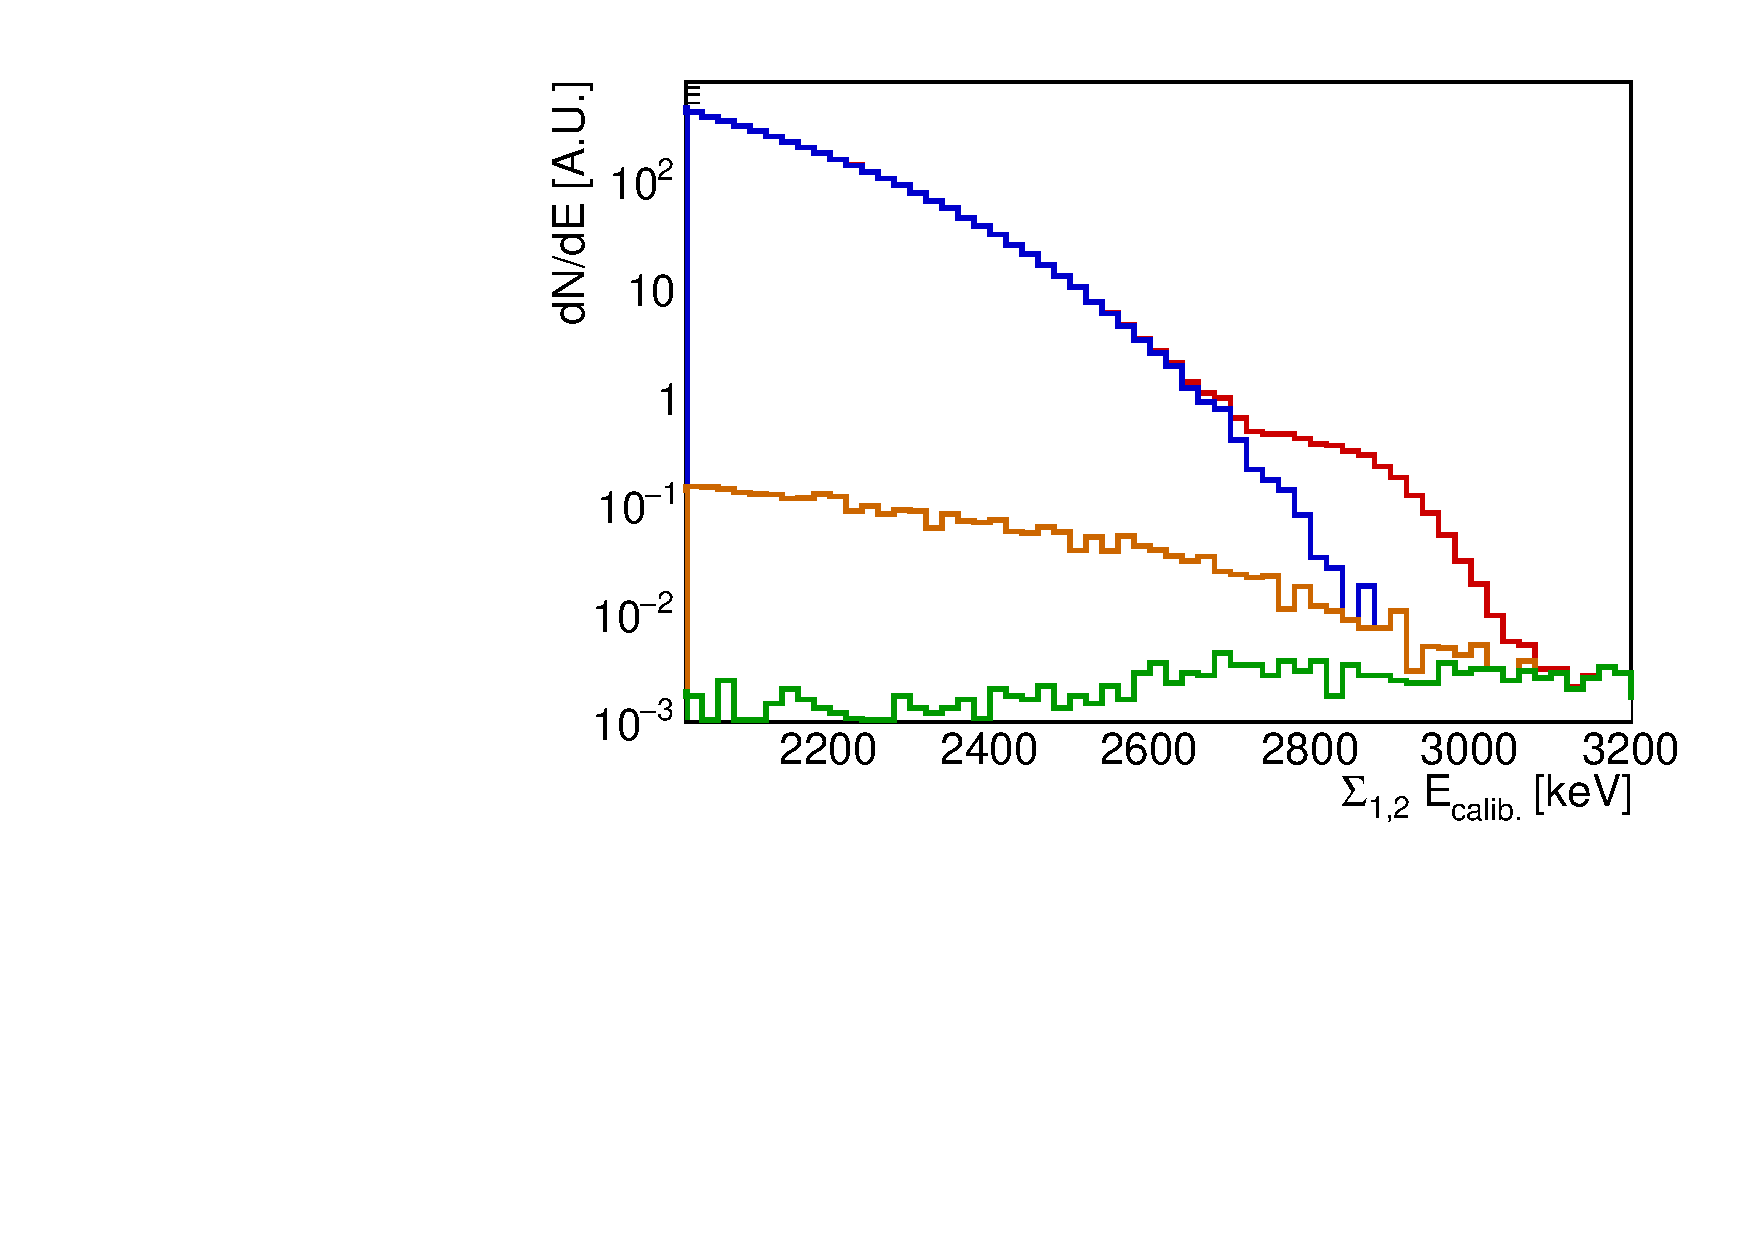
\includegraphics[scale=0.60]{pictures/Chap5/tot_energy_spectrum.pdf}
%\caption{Energy spectrum of the sum of the 2 electrons for the $\beta \beta 0 \nu$ signal (red) and the different backgrounds ($\beta \beta 2 \nu$ in blue, $^{214}Bi$ in orange and $^{208}Tl$ in green). The energy spectrum takes the SuperNEMO detector response into account.}
%\label{energySpectrum}
%\end{center}
%\end{figure}


\NI As discussed in Chapter~\ref{chap:NEMO}, the $\beta\beta$ process is very rare and its study requires a very low background environment. The detectors searching for $\beta\beta$ decays are installed in underground laboratories and protected with different shields to be sheltered against the cosmic ray and the photon/neutron fluxes coming from the laboratory.


\bigskip


\NI Despite these precautions, some backgrounds can still be present and bother the $\beta\beta$ searches. One of the main background is induced by radon. Radon ($^{\text{222}}$Rn) is a highly diffusive gas emanating from the rocks surrounding the underground laboratory. At LSM, its activity in the surrounding air has been measured to be~10Bq/m$^\text{3}$~\cite{RadonLSM}. The descendants of the $^{\text{222}}$Rn, mainly the $^{\text{218}}$Po, could deposit themselves on the tracker wires or on the surface of the source foil. As shown in Figure~\ref{Radon222decayChain}, $^{\text{222}}$Rn reaches during its decay chain, the $^{\text{214}}$Bi isotope which is one of the main backgrounds in the NEMO experiments due to the electron emitted at 3.27~MeV. Figure~\ref{Backgroungs} shows how the decay of $^{\text{214}}$Bi can by different processes (Möller scattering or Compton effect) mimic the $\beta\beta$ signal. 


\bigskip


\noindent From the NEMO-3 to the SuperNEMO experiments, the aim is to reduce the $^{\text{222}}$Rn contamination inside the tracker by a factor~50. The following techniques will be employed :


\begin{itemize}

\item Improve the radiopurity of each components avoiding $^{\text{222}}$Rn emanation coming from the detector itself.

\item Install an anti-radon system made of a clean tent which surrounds the entire detector hermetically and filters the air inside the tent with a radon trap. 

\end{itemize}


\begin{figure}[h!]
\begin{center}
\includegraphics[scale=0.3]{pictures/Chap5/Radon222decayChain.png}
\caption{$^{\text{222}}$Rn decay chain.}
\label{Radon222decayChain}
\end{center}
\end{figure}


\begin{figure}[h!]
\begin{center}
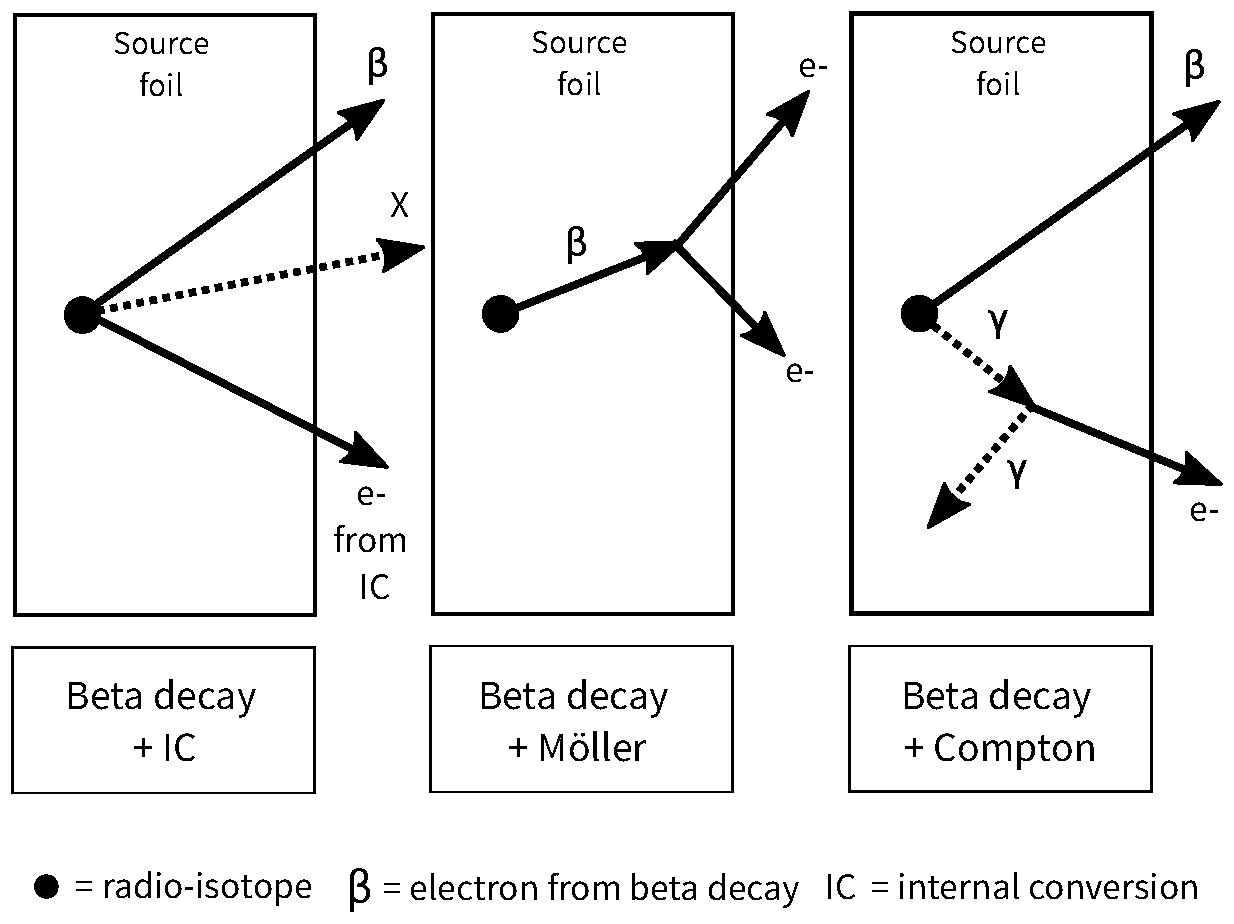
\includegraphics[scale=0.4]{pictures/Chap5/internal_bkg.pdf}
\caption{Background processes coming from the foil which mimic the two electron events. On the left : beta decay and internal conversion. In the center : beta decay and M\o ller scattering. On the right : beta decay and Compton scattering.}
\label{Backgroungs}
\end{center}
\end{figure}


\noindent Despite the good radiopurity of the components and the anti-radon system, some residual contamination of $^{\text{222}}$Rn is expected in the tracker volume. In order to identify and suppress these remaining events, analysis tools have been implemented. The strategy is to use the fact that $^{\text{214}}$Po, the daughter nucleus of $^{\text{214}}$Bi, is not stable. The $^{\text{214}}$Po nucleus decays to $^{\text{210}}$Pb by emitting an alpha particle with a half-life of 164.6~$\pm$~0.3~$\mu$s~\cite{NuclearDataSheet210} as shown in Figure~\ref{BiPoChain}. The reconstruction of these events, called BiPo events, with the characteristic coincidence time among the prompt electron and the delayed alpha provides a very clean and sensitive way to measure the $^{\text{214}}$Bi/$^{\text{222}}$Rn contamination in the detector.   


\begin{figure}[h!]
\begin{center}
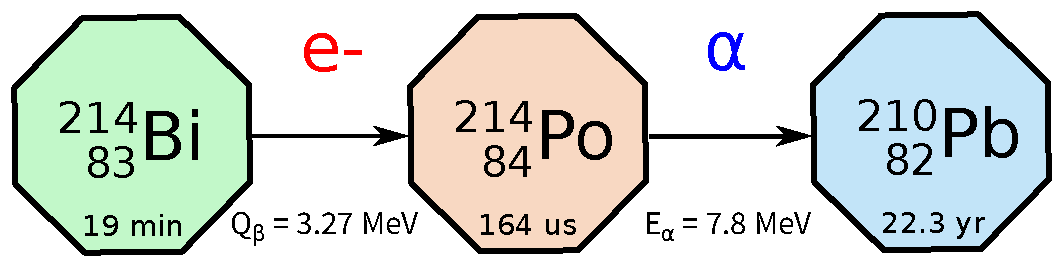
\includegraphics[scale=0.6]{pictures/Chap5/decay_chain_bi.pdf}
\caption{The $^{\text{214}}$Bi decay chain. The first decay emits an electron with Q$_{\beta} =$ 3.27 MeV. The daughter $^{\text{214}}$Po then decays by emitting a monoenergetic alpha particle, $\text{E}_{\alpha} =$ 7.8 MeV. The half-life of $^{\text{214}}$Po is 164.6~$\pm$~0.3$\mu$s.}
\label{BiPoChain}
\end{center}
\end{figure}


\bigskip


\NI The number of expected events coming from $^{\text{214}}$Bi, can be estimated, for each part i of the detector by using :


\begin{equation}
(\text{N}_{\text{1e1}\alpha})_\text{i} = (\epsilon_{\text{1e1}\alpha})_\text{i} \times \text{A}_\text{i} \times \text{T}
\label{eq_number_of_expected_events}
\end{equation}


\noindent where $(\epsilon_{\text{1e1}\alpha})_\text{i}$ is the efficiency of selecting 1e1$\alpha$ events (which has to be determined by simulations), A$_\text{i}$ is the activity of the component of the detector which has been previously measured and T is the time of exposure. 


\bigskip


\NI Section~\ref{sec:ActivityComputation} presents the computations of the expected activities in the different parts of the detector from the radiopurity measurements.  Section~\ref{sec:SimuReco} introduces the simulation and the reconstruction tools used in this study. Section~\ref{sec:ReconstructionAlphaParticle} presents the algorithm developped in this work to identify and reconstruct the alpha particles. The selection and the efficiency of reconstruction of the 1e1$\alpha$ channel are presented in Section~\ref{sec:Selection1e1aChannel}. Section~\ref{sec:MeasurementStategy} explains the strategy used to estimate the level of background induced by $^{\text{222}}$Rn and with what precision it can be measured. Section~\ref{sec:Results} presents the results of this work.


\FloatBarrier


%----------------------------------------------------------------------------------------
%   ACTIVITIES COMPUTATION
%----------------------------------------------------------------------------------------


\section{Computation of the expected activity}\label{sec:ActivityComputation}


\NI By knowing the $^{\text{214}}$Bi contamination of the different detector components and their mass or volume, the activity of $^{\text{214}}$Bi can be evaluated for each of these parts. Sections~\ref{sec:ActivitySourceFoil} and~\ref{sec:ActivityTracker} respectively present the activity computations for the contamination coming from the source foil and from the tracker.  


\subsection{Activity source the foil}\label{sec:ActivitySourceFoil}


\noindent $^{\text{214}}$Bi contamination expected from the source foil has been measured in the BiPo detector. Results presented in~\cite{BiPoResultsGomez,BiPoResultsLoaiza} put an upper limit on the total activity of 2200 $\times$ 10$^{-\text{6}}$~Bq/kg for the $^{\text{82}}$Se and 210 $\times$ 10$^{-\text{6}}$~Bq/kg for the raw mylar.  


\bigskip


\noindent Thanks to these measurements, the radiopurity of each component used in the source foil fabrication is known. By assuming that the bulk of the foil is only made up of~$^{\text{82}}$Se and the surface of the foil is made up of only raw mylar, the total activity can be computed in each part of the detector : 

\begin{itemize}
\item the bulk of the foil :
\begin{equation}
\text{A}_{\text{bulk}} =  \text{2200} \times \text{10}^{-\text{6}}~ \text{Bq/kg} \times \text{7}~\text{kg} = \text{15.4}~\text{mBq} 
\end{equation}

\item the surface of the foil :
\begin{equation}
\text{M}_{\text{surface}} = \text{2}~\text{sides} \times \rho \times \text{V} = \text{2} \times \text{1.40} \text{g/cm}^\text{3} \times \text{314.7} \text{cm}^\text{3} = \text{0.88}~\text{kg}
\end{equation}

\begin{equation}
\text{A}_{\text{surface}} = \text{210} \times \text{10}^{-\text{6}}~\text{Bq/kg} \times \text{0.88}~\text{kg} = \text{0.18}~\text{mBq} 
\end{equation}
\end{itemize}


\NI where A$_{\text{bulk}}$ and A$_{\text{surface}}$ are the bulk and surface activities of the source foil, M$_{\text{surface}}$ is the mass of the mylar computed as the product of its density $\rho$ and its volume V.


\subsection{Activity from the tracker}\label{sec:ActivityTracker}


\noindent The intrinsic tracker activity has been measured using a RAD7 detector at MSSL~\cite{RAD7measurement}. By assuming that the air is not flushing and that the contamination is 4 times the contamination of the C0 section measured at 11.37~mBq, the activity of the tracker is evaluated to be : 


\begin{equation}
\text{A}_{\text{tracker}} =  \text{4} \times  \text{11.37} = \text{45.5}~\text{mBq} 
\end{equation}


\NI This value of $\text{45.5}~\text{mBq}$ for the tracker activity is probably an overestimation since C1 and C2 sections have been measured respectively at 15.2~mBq and 3.28~mBq as reported in Table~\ref{tab:RadonEmanation}. Calculating the mean value of these measurements gives 10~mBq/C-section corresponding to a total expected activity of 40~mBq for the tracker. Futhermore, the fact that a certain amount of $^{\text{222}}$Rn present in the tracker contaminates the surface of the foil is not taken into account, which would decrease the tracker activity. In addition, the activity inside the tracker can be reduced by flushing the air inside the tracker chamber. Despite this approximation, the value of $\text{45.5}~\text{mBq}$ is chosen for this study since it is probably not so far from the real value (C3 has not been measured) and that we want to test the measurement method. The total activities of each part of the detector (source and tracker) are summarized in the Table~\ref{activity_measurement_different_parts}.


\begin{table}[h!]
\begin{center}
\begin{tabular}{c|c|c|c}
               & Bulk & Surface & Tracker \\[0.1cm]
\hline
Activity [mBq] & 15.4 & 0.18    & 45.5    \\[0.1cm]
\hline
\end{tabular}
\end{center}
\caption{Summary of the total activity, in different parts of the detector, computed from the radiopurity measurements.}
\label{activity_measurement_different_parts}
\end{table}


%----------------------------------------------------------------------------------------
%   SIMULATION AND RECONSTRUCTION
%----------------------------------------------------------------------------------------

\section{Simulation and Reconstruction}\label{sec:SimuReco}


\noindent The simulation and reconstruction tools used in this work are available in the software package developped by the collaboration called Falaise (version 1.0.0). The simulations of the events is done by GENBB and presented in Section~\ref{sec:GenerationBi214}. The propagation of the particle inside the SuperNEMO detector is done by GEANT4 and introduced in Section~\ref{sec:DectectorResponseBi214}. For the reconstruction, each event is processed through a pipeline consisting of a sequence of software modules as discussed in Section~\ref{sec:ReconstructionBi214}. Each module is responsible for the elaboration of additional information stored in dedicated banks. An additional tool giving interesting variables on standard ROOT trees is developed for an easier access to the simulated and reconstructed information.


\subsection{Generation of the $^{\text{214}}$Bi events}\label{sec:GenerationBi214}


\noindent The first step is the generation of $^{\text{214}}$Bi events with the simulation software. In this chapter, the events are generated at the surface of the source foil, in the bulk of the source foil and in the tracker volume. The event generation is done by GENBB and the propagation of the particles into the SuperNEMO detector is realized by GEANT4~\cite{GEANT4}.


\bigskip


\noindent GENBB is a Monte-Carlo event generator for double beta processes and the decay of radioactive nuclei. It can generate the decay ($\alpha$, $\beta^\pm$, electron conversion) of all known isotopes by taking into account the information of the decays (decay mode, energy release, transition probability, half-life...). Transitions to the ground state as well as to excited levels of daughter nuclei are allowed. GENBB generates the energy, the time of decay and the direction of emitted particles.


\bigskip 


\noindent In this work, the generation is performed in agreement with the decay scheme of $^{\text{214}}$Bi. Since GENBB also simulates secondary nuclear effects such as internal conversion or decay via the excited state, the consequence is the generation of different topologies :


\begin{itemize}
\item The 1e1$\alpha$ topology, which represents 18.2$\%$ of all the simulated topologies, corresponds to the standard (BiPo) decay. The $^{\text{214}}$Bi decays to the ground state of $^{\text{214}}$Po.


\item The 1e1$\alpha$n$\gamma$ topologies, which represent 79.1$\%$ of all the simulated topologies, correspond to the BiPo decay accompanied by a gamma emission. In this case, the $^{\text{214}}$Bi decays to an excited state of $^{\text{214}}$Po and a gamma or a cascade of gammas is then produced.


\item The 2e1$\alpha$n$\gamma$, 3e1$\alpha$n$\gamma$, 4e1$\alpha$n$\gamma$ topologies, which represent 2.58$\%$ of all the simulated topologies, correspond to a BiPo event with an internal conversion~(IC). An excited $^{\text{214}}$Bi nucleus can directly transfer its energy to an orbital electron. This electron is expelled from the atom with a discrete energy. The direct consequence is the generation of more than one electron in the event, which could mimic 2e$^-$ event from $\beta\beta$ decay.


\end{itemize}


\noindent In any case, whatever the topology, an alpha is always present. This justifies its search and why the 1e1$\alpha$ channel is an appropriate channel to detect the $^{\text{214}}$Bi.


\bigskip

 
\noindent A way to quantitatively ensure that these electrons really come from internal conversions is to analyze the energy spectrum of all the simulated electrons as shown in Figure~\ref{energyspectrumallelectron}. The shape of the energy spectrum of the emitted electrons from $^{\text{214}}$Bi beta decay is well recognizable with a Q$_\beta$ at 3.27~MeV. The sharp overlapping peaks correspond to the monoenergetic electrons emitted from internal conversions. 


\bigskip

\noindent By removing the contribution of the electrons coming from the $\beta$ decay, only the electrons coming from internal conversions are kept. Figure~\ref{energyspectrumallelectron} shows the energy spectrum of these electrons normalized to the number of total events. The four main peaks observed at 0.516, 0.592, 1.027 and 1.322~MeV correspond to the internal conversion of $^{\text{214}}$Bi. Table~\ref{internalconversioncomparaison} shows the intensity comparision between the published values \cite{NuclearDataSheet210} and the values obtained in this study which agree rather well.


\bigskip


\noindent The above channels are the predominant ones in the decay of the $^{\text{214}}$Bi. Alongside these there are also a few much less probable final states such as $\alpha-$decay of $^{\text{214}}$Bi (1$\alpha$, 1$\alpha$1$\gamma$,..) or other channels with positron emissions (2e1$\alpha$1p). Table \ref{1e1atopology} summarizes all the topologies created by GENBB during the simulation of the $^{\text{214}}$Bi decay.


\begin{table}[h!]
\begin{center}
\begin{tabular}{c|c|c}
Electron energy [MeV]  & published values & this study \\[0.1cm]
\toprule
0.516  & 0.676 $\pm$ 0.010 \% & 0.688 $\pm$ 0.015 \% \\[0.1cm]
0.592  & 0.189 $\pm$ 0.003 \% & 0.210 $\pm$ 0.008 \% \\[0.1cm]
1.027  & 0.186 $\pm$ 0.003 \% & 0.198 $\pm$ 0.008 \% \\[0.1cm]            
1.322  & 0.480  & 0.493 $\pm$ 0.013 \% \\[0.1cm]
\bottomrule
\end{tabular}
\end{center}
\caption{Comparison of the intensities of the four main peaks due to internal conversion electrons.}
\label{internalconversioncomparaison}
\end{table}


\begin{figure}[h!]
\begin{center}
%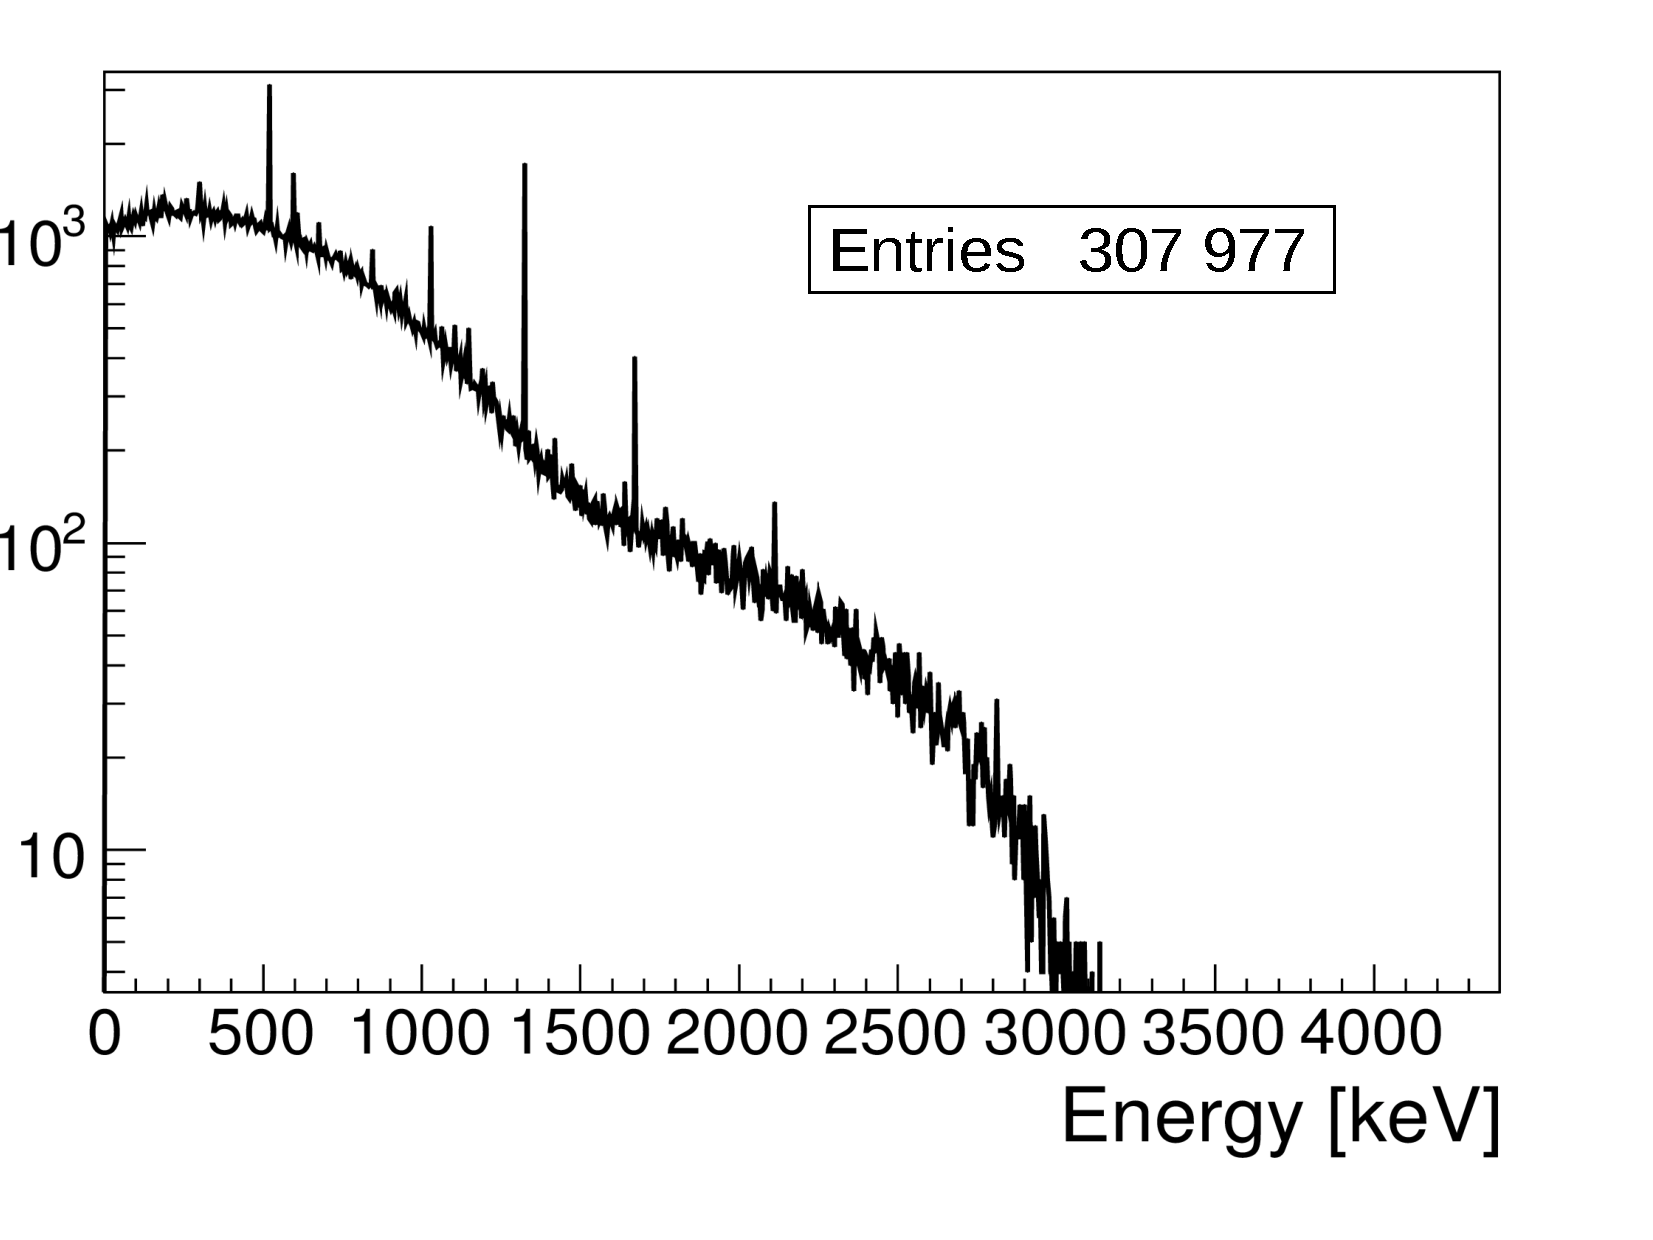
\includegraphics[scale=0.25]{pictures/Chap5/energy_spectrum_all_electron.pdf}
\includegraphics[scale=0.28]{pictures/Chap5/energy_spectrum_internal_conversion_v3.pdf}
\caption{Left : Energy spectrum of all simulated electrons. The shape of the energy spectrum of the $^{214}$Bi beta decay is well recognizabe with a Q$_\beta$ of 3.27~MeV. The sharp peaks correspond to the monoenergetic electrons emitted from internal conversions. Right : Energy spectrum of the electrons emitted in internal conversions normalized to the number of total simulated events.}
\label{energyspectrumallelectron}
\end{center}
\end{figure}


%\begin{figure}[h!]
%\begin{center}
%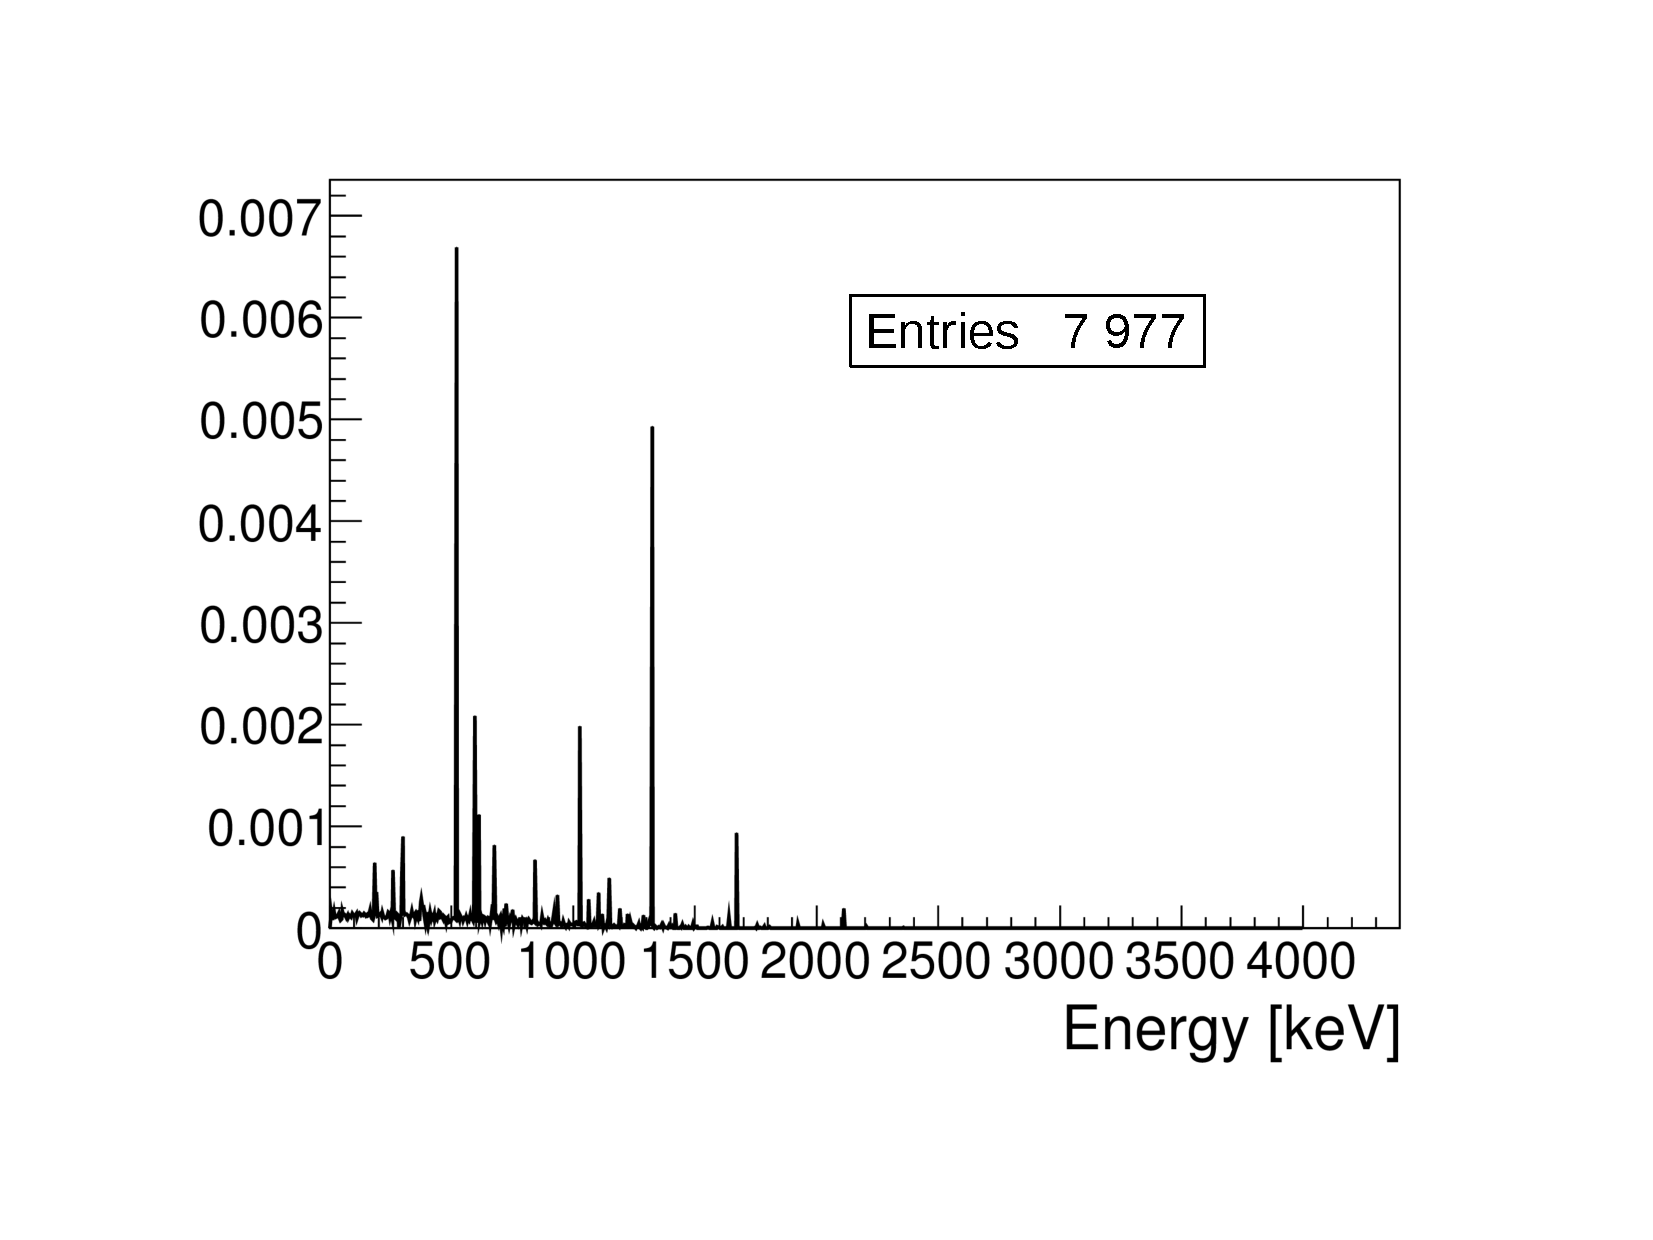
\includegraphics[scale=0.43]{pictures/Chap5/energy_spectrum_internal_conversion.pdf}
%\caption{Energy spectrum of the electrons emitted in internal conversions normalized to the number of total simulated events.}
%\label{energyspectruminternalconversion}
%\end{center}
%\end{figure}


\begin{table}[h!]
\begin{center}
\begin{tabular}{l|l|c|c}
\toprule
    & Simulated topology & 300 000 & 100 $\%$ \\[0.1cm]
\hline
                           &1$\alpha$            & 21      & 0.007 \%  \\
$^{\text{214}}$Bi $\alpha-$ decay &1$\alpha$1$\gamma$   & 9       & 0.001 \%  \\
                           &1$\alpha$2$\gamma$   & 2       & 0.0006 \% \\[0.1cm]
\hline
                           &1e1$\alpha$          & 54 592  & 18.2 \%   \\
BiPo decay                 &1e1$\alpha$1$\gamma$ & 101 304 & 33.8 \%   \\
ground and excited         &e1$\alpha$2$\gamma$  & 122 765 & 40.9 \%   \\
states                     &1e1$\alpha$3$\gamma$ & 12 994  & 4.3 \%    \\
                           &1e1$\alpha$4$\gamma$ & 426     & 0.14 \%   \\
                           &1e1$\alpha$5$\gamma$ & 1       & 0.0003\%  \\[0.1cm]
\hline
                           &2e1$\alpha$1$\gamma$ & 1266    & 0.4 \%    \\
                           &2e1$\alpha$2$\gamma$ & 5052    & 1.7 \%    \\
                           &2e1$\alpha$3$\gamma$ & 1313    & 0.4 \%    \\
BiPo with IC               &2e1$\alpha$4$\gamma$ & 107     & 0.04 \%   \\
                           &3e1$\alpha$2$\gamma$ & 91      & 0.03 \%   \\
                           &3e1$\alpha$3$\gamma$ & 30      & 0.01 \%   \\
                           &3e1$\alpha$4$\gamma$ & 2       & 0.0006 \% \\
                           &4e1$\alpha$3$\gamma$ & 2       & 0.0006 \% \\[0.1cm]
\hline 
                           &2e1$\alpha$1p          & 17    & 0.006 \% \\
others                     &2e1$\alpha$1p1$\gamma$ & 6     & 0.002 \% \\[0.1cm] 
\bottomrule
\end{tabular}
\end{center}
\caption{The topology of the events simulated during the decay of $^{\text{214}}$Bi}
\label{1e1atopology}
\end{table}


\FloatBarrier


\subsection{Detector response simulation}\label{sec:DectectorResponseBi214}


\noindent The second step is the GEANT4 simulation of the detector response. A brief reminder of the SuperNEMO geometry useful to this work are presented here. The response of the tracker and the calorimeter is done within the Calibration module.


\bigskip


\noindent The tracker, that sandwiches the source foil, is composed of 2034 Geiger cells (9 layers and 113 rows). Each Geiger cell is composed of an anodic wire and 8 cathodic wires for a total of 18306 wires. The distance between each Geiger cell is~2.1~cm.


\bigskip


\noindent The calorimeter is composed of 6 walls : 2 main walls on opposite sides of the source foil, 2 $\gamma$-vetos and 2 x-walls to cap the sides, the top and the bottom of the detector. Each main wall has 260 optical modules made of Polystyrene scintillator blocks directly coupled to a 8-inch low radioactivity PMT. The mean energy resolution of the optical modules, at 1MeV, is $\sim$8\%. The distance between the source foil and the main wall is~45~cm.   


\bigskip


\noindent The response of the calorimeter is simulated though a Gaussian smearing of the true energy taking into account the energy resolution of the calorimeter. The transverse drift radius of the Geiger cells is simulated according to the relation beetween the drift time and radius plotted in Figure~\ref{drift_time}~\cite{DriftTimeModel}. This module creates and fills the Calibrated Data (CD) bank.


\begin{figure}[h!]
\begin{center}
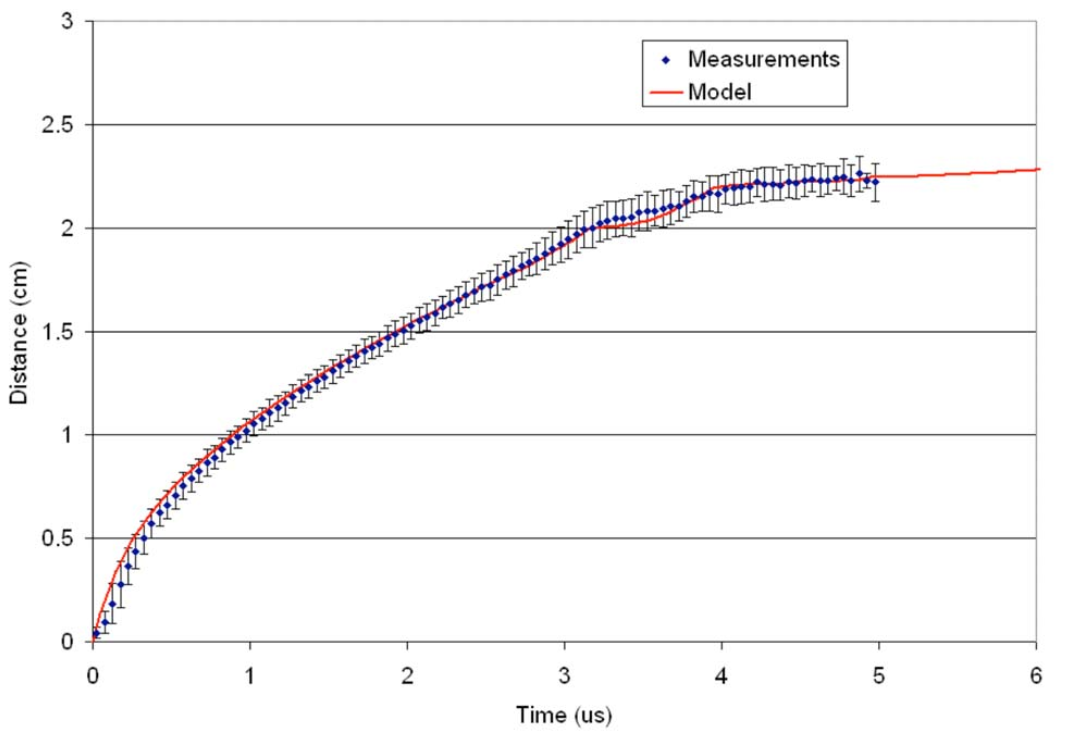
\includegraphics[scale=0.25]{pictures/Chap5/drift_time.png}
\caption{The relation between the transverse drift time and drift radius}
\label{drift_time}
\end{center}
\end{figure}


\FloatBarrier


\subsection{Reconstruction of the simulated events}\label{sec:ReconstructionBi214}


\noindent The third and last step is the reconstruction of the simulated events. The list of modules processed in the pipeline used in this study are given below : 


\begin{itemize}


\item \textbf{Cellular Automaton Tracker (CAT)} : this module clusters the calibrated Geiger hits. It creates and fills the Tracker Clustering Data (TCD) bank. The TCD bank contains all the cluster information. The clusterisation runs in two steps. The first step is to perform a pre-clusterisation. CAT sorts the Geiger hits according to the drift time. If the drift time is smaller than 10 $\mu$s from the time of the first particle emission, the cluster is considered as prompt, otherwise it is considered as delayed. The two samples of Geiger hits are then treated separately. The second step is the clusterisation of the Geiger hits by taking into  account their proximity in space through a cellular Automaton Algorithm. %More detailed documents on CAT can been found in \cite{CAT}.

\item \textbf{TrackFit} : this module fits the clusters found by CAT. It creates and fills the Tracker Trajectory Data (TTD) bank. The TTD bank contains all the track information. The fitting algorithm tries to fit a straight line or a helix to the cluster. If the cluster is better approximated by a staight line fit, the track is defined by 2 parameters : the first and the last points of the line. In case a helical trajectory is fitted, the track is defined by 5 parameters : the center, radius, pitch and first and last angles of the helical segment. Due to the minimum number of degrees of freedom required to fit a straight line, TrackFit considers only clusters containing 3 or more Geiger hits. TrackFit is also able to estimate the alpha emission time which is in practice unknown. %See \cite{TrackFit} for more informations. % By default, only the prompt clusters are fitted. To take into account the delayed clusters the pipeline configuration has to be modified.

\item \textbf{Charge Particle Tracking} : this module creates and fills the Particle Track Data (PTD) bank. It computes for each track the charge according to the curvature from the magnetic field.  Charged Particle Tracking also extrapolates the track to estimate its vertex. If the layer of the wires nearest the foil source is triggered, the vertex is extrapolated onto the source foil. In the same way, if a calorimeter hit occurs close to a track and if the layer of wires nearest this calorimeter block have been triggered, the track is extrapolated to the surface of the calorimeter block.
%See \cite{ChargedParticleTracking} for more informations.
\end{itemize}


\noindent Others modules have been developed and are used for the reconstruction of the different channels. They are briefly described here :


\begin{itemize}


\item \textbf{Particle Identification module} : this module tags the reconstructed particles according to definitions given by the user. If a particle meets the requirements defined to be an electron the particle is tagged and fills the electron bank. %The definitions are given in a configuration file as cuts. To be accepted in the electron or in the alpha bank, the particle must respect some criteria given by the user. 


\item \textbf{Topology module} : this module creates a new data bank called Topology Data (TD). The particles in an event are associated to form a topology. This module computes some observables of the reconstructed topology : 

 
\begin{itemize}


\item the time of flight from the foil to calorimeter
\item the angle $\theta$ between the particles at the emission vertex
\item the difference in vertex positions on the foil
\item The delay time between the electron and the alpha ($\Delta t_{e-\alpha}$)
\item The Y, Z and YZ distances between the two extrapolated vertices on the source foil
\item The X, Y and Z distance between the two nearest Geiger hits to the source foil.


\end{itemize}


\item \textbf{Process 1e1$\alpha$ topology cut} : specific to this work, this module recognizes the 1e1$\alpha$ topology among all the rest.% and executes different actions for these events.


\item \textbf{Output module} : this last module is responsible for storing the simulated and reconstructed information in a ROOT tree.


\end{itemize}


\FloatBarrier


%----------------------------------------------------------------------------------------
%    RECONSTRUCTION OF THE ALPHA PARTICLE
%----------------------------------------------------------------------------------------


\section{Reconstruction of the $\alpha$ particle}\label{sec:ReconstructionAlphaParticle}


Because of its high ionization power, the energy loss of an alpha is much larger than that of an electron. The stopping power (-dE/dx) for an alpha particle, in a gas made of 100 \% of He, is $\sim$~0.25 MeV/cm. In other words, the typical path length of an alpha with an energy equal to 7.8~MeV does not exceed 40~cm. So an alpha coming from the source foil is not expected to hit the main calorimeter wall. Due to their high mass, alpha particles are not significantly affected by the magnetic field so their tracks will be essentially straight lines. An alpha particle is then identified as a short straight line of Geiger hits delayed in time with respect to the electron. A visualisation of a typical alpha track coming from the source is shown in Figure~\ref{visu_alpha_typical_track}.


\begin{figure}[h!]
\begin{center}
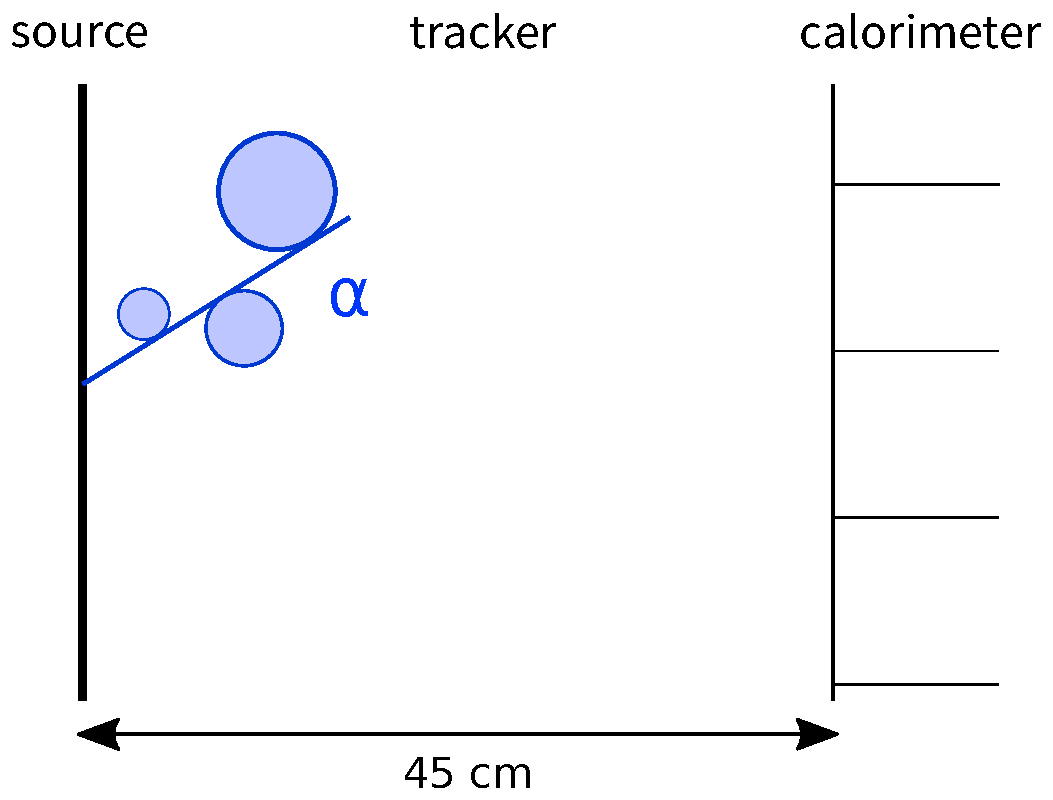
\includegraphics[scale=0.50]{pictures/Chap5/alpha_comic.pdf}
\caption{Visualisation of a typical alpha track coming from the source. The blue circles represent the Geiger hits and the straight line the fitted track.}
\label{visu_alpha_typical_track}
\end{center}
\end{figure}


\subsection{The Alpha Finder algorithm}


\noindent The typical alpha track is a delayed short and straight line. Some alphas can have only 1 or 2 Geiger hits, these alphas could otherwise be lost because they are not fitted by TrackFit. For this reason, an algorithm, called Alpha Finder, was developed. Its goal is to search for delayed non-clustered (single) hits and the delayed non-fitted (double) hits. The algorithm is based on the algorithm developed for NEMO-3 and is described here. %The algorithm is based on Vera's algorithm and the work of S.Torre \& J.Mott work for the NEMO-3 experiment \cite{AlphaFinderNEMO3}. 


\bigskip


\noindent In each event, the presence of a prompt electron track is checked. It is important to verify the presence of a prompt track because, later, during data taking, a window of 1~ms will be opened just after a calorimeter hit triggered by a prompt track. If the event contains a prompt track, the presence of delayed unfitted tracks (a 2 hit cluster) or delayed unclustered Geiger hit (a single hit) is verified.


\bigskip


\noindent Once we are sure that the event contains such ignored delayed Geiger hits, their X,Y and Z position and their time are stored. To be accepted, the delayed Geiger hit(s) must fulfill some requirements :


\begin{itemize}


\item the delayed time of the delayed Geiger hits has to be greater than a certain time defined by the \begin{ttfamily}minimum$\_$delayed$\_$time\end{ttfamily}. The CAT algorithm considers a hit as delayed if the delayed time is greater than 10 $\mu$s. The same time has been chosen for the Alpha Finder.


\item the distance in XY between the delayed hit(s) and the hits of the prompt track is computed, and must be smaller than a certain distance called \\
\begin{ttfamily}minimal$\_$cluster$\_$xy$\_$search$\_$distance\end{ttfamily}. The default value has been set at 40 cm.


\item the same distance is computed for the Z axis,and must be smaller than \\
 \begin{ttfamily}minimal$\_$cluster$\_$z$\_$search$\_$distance\end{ttfamily}. The default value has been set at 30 cm.


\item Finally, the distance between the delayed hit(s) and the vertex of the prompt track is also computed. The distance has to be smaller than a certain distance called \begin{ttfamily}minimal$\_$vertex$\_$distance\end{ttfamily}. The default value has been set to 30 cm.


\end{itemize}


\noindent If all these different criteria are fulfilled, the delayed cluster (2 hits) or the single hit are added to the alpha bank along with their properties (delayed time, X,Y and Z position...). The delayed time of the alpha corresponds to the delayed time of the Geiger cell which is known with an uncertainty of 4 $\mu$s. 4$\mu$s corresponds to a drift radius of 2.2 cm which is a Geiger cell radius. 


\bigskip


\noindent In the case of just one delayed hit, the length of the alpha track is set by computing the distance between the vertex extrapolation of the prompt track and the center of the delayed cell. In the case of 2 delayed hits, the length of the alpha track is set by computing the distance between the vertex extrapolation of the prompt track and the center of the furthest delayed cell.


\bigskip


%\noindent The selection parameters can easily be changed in the pipeline configuration file in the section dedicated to the ChargedParticleTracking. 
\NI To summarise, there are two ways to find the alpha particles. The alpha particles with 3 or more Geiger hits (long alpha)  are found by CAT while the alpha particles with 2 or fewer Geiger hits (short alpha) are found by the Alpha Finder. During the reconstruction of the 1e1$\alpha$ channel, long and short alpha particles are treated equally, whatever the way they have been found.

  
%-------------------------------------------------
\subsection{The alpha emission time $t_0$}


To find the radius of a Geiger cell, the drift time has to be known. For the prompt tracks it is quite easy to recover the drift time. In an event, the anodic time ($\text{t}_{\text{A}e}$) corresponds to the electron emission time ($ \text{t}_e$) plus the drift time ($\text{t}_d$) :


$$\text{t}_{\text{A}e} = \text{t}_e + \text{t}_d$$


\noindent The electron emission time corresponds within a few ns to the time when the electron hits the calorimeter wall. The response of the calorimeter is very quick (few ns). The anodic time is given by the tracker. The response of the tracker is slower than the calorimeter. In this way, the drift time can be calculated. The correspondence between drift time and the radius has been measured and is given in Figure~\ref{drift_time}.


\bigskip


\noindent For the delayed tracks, it is a little bit different. The anodic time ($\text{t}_{\text{A}\alpha}$) corresponds to the electron emission time ($ \text{t}_e$) plus the alpha emission time ($ \text{t}_\alpha$) plus the drift time ($\text{t}_d$). 


$$\text{t}_{\text{A}\alpha} = \text{t}_e + \text{t}_\alpha + \text{t}_d$$


\noindent In practice the alpha emission time is unknown. Nevertheless, a solution has been found to estimate this time. The trick is to consider the alpha emission time as a parameter of the fit of the track (done by Trackfit) to the following expression :


$$\text{t}_{\text{A}\alpha} - \text{t}_\alpha =  \text{t}_e  + \text{t}_d$$


\noindent In Figure \ref{timeReco}, the difference $\Delta$t$_\text{0}$ between the true alpha emission time and the reconstructed alpha emission time is plotted. A picture of the visualisation is also shown in the Figure \ref{timeRecovisu}. The agreement between the reconstruction and the simulation is correct and accurate enough for the following studies presented in this chapter. The more the number of Geiger hits in the track the better the $\alpha$ emission time is reconstructed. If the number of Geiger hits in a cluster is equal to 2 or less, this calculation is not done because it relies on the fitting of the tracks. 


\begin{figure}[h!]
\begin{center}
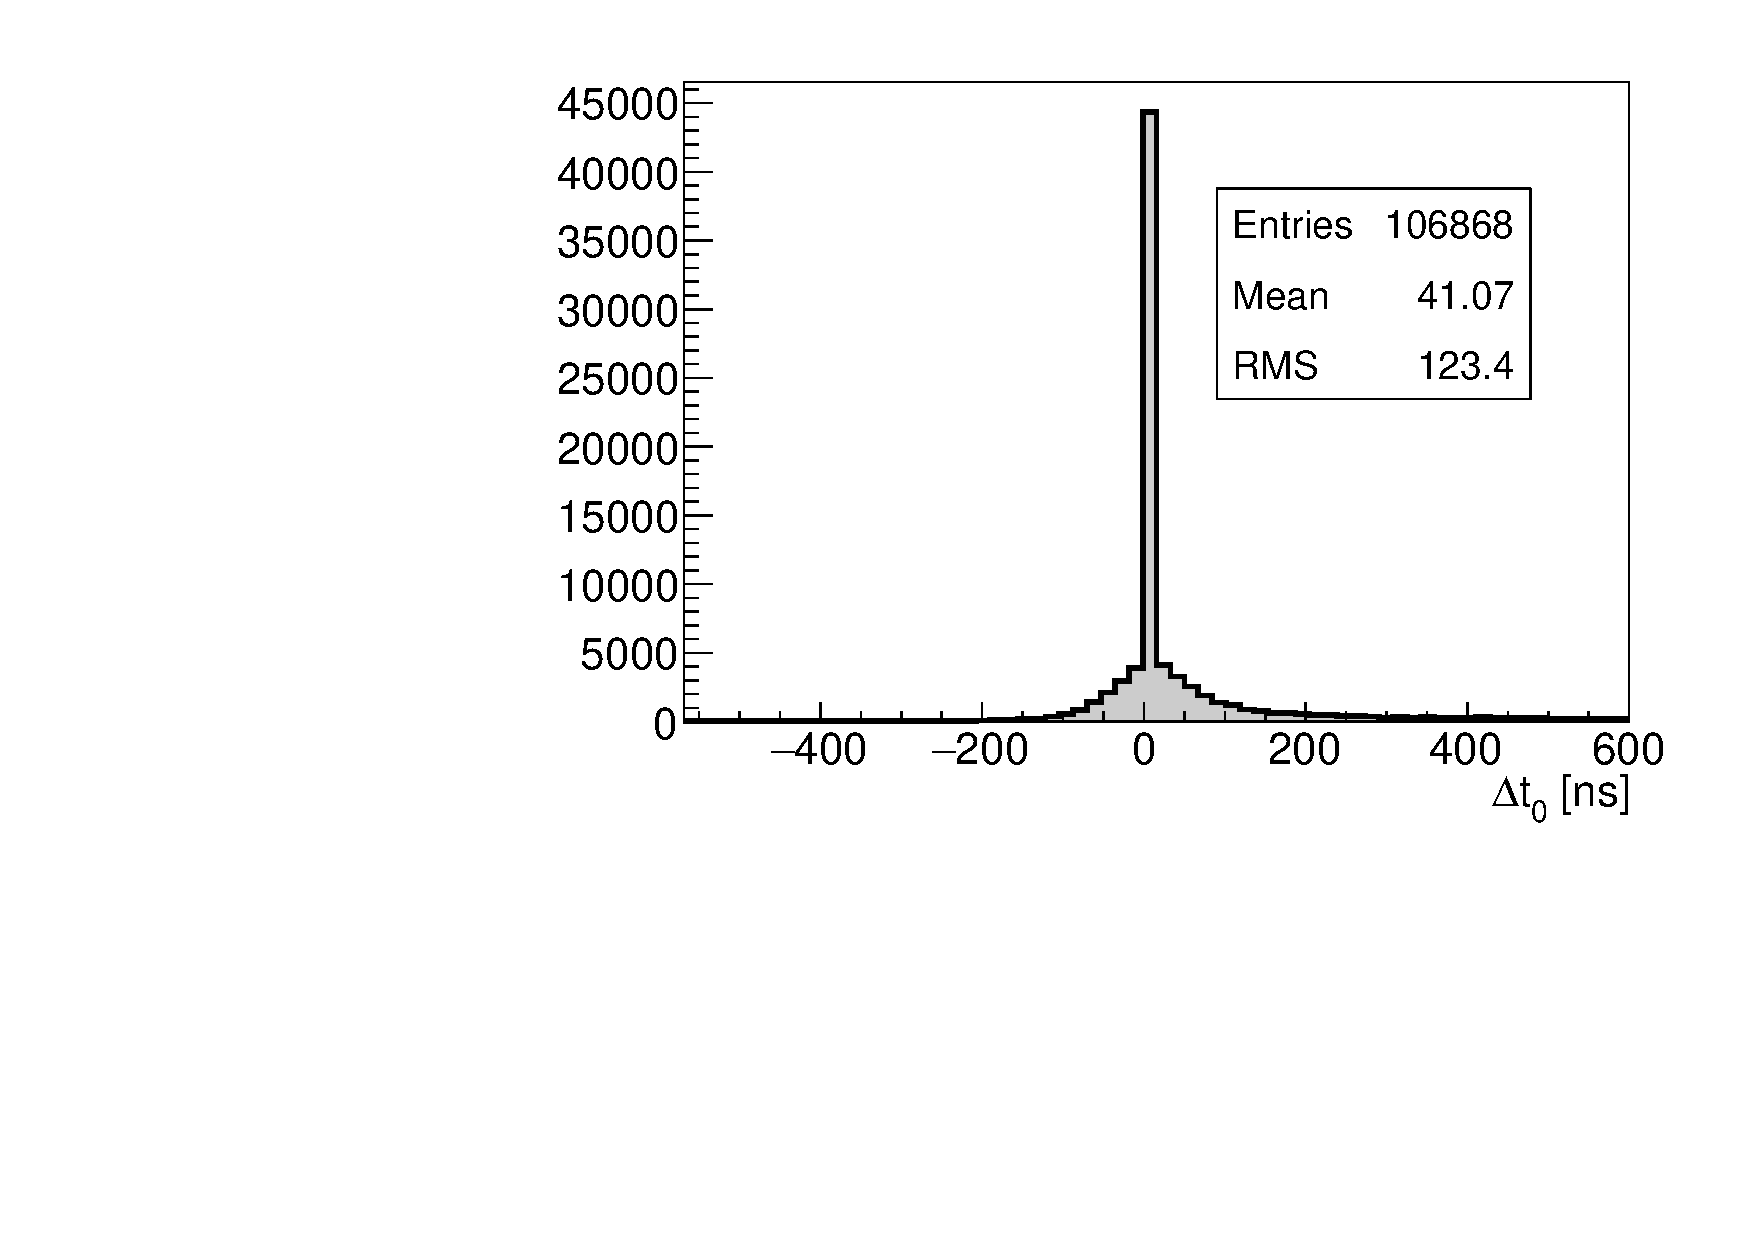
\includegraphics[scale=0.55]{pictures/Chap5/delta_time_simu_reco.pdf}
\caption{The difference between the true alpha emission time and the reconstructed alpha emission time. The distribution is peaked at 0 showing that the reconstruction and the simulation are in good agreement.}
\label{timeReco}
\end{center}
\end{figure}


\begin{figure}[h!]
\begin{center}
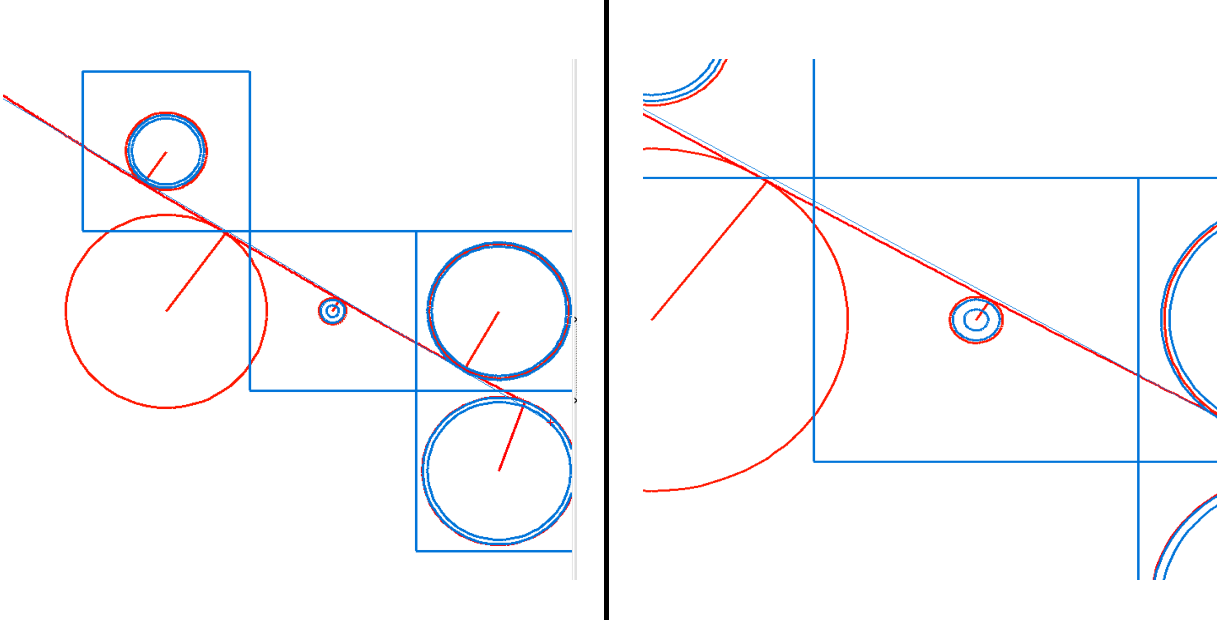
\includegraphics[scale=0.6]{pictures/Chap5/dessin.pdf}
\caption{Visualisation of simulated (red) and reconstructed (blue) alpha. On the left, a global view is shown, on the right, a zoomed view of the same event is presented. In the simulation, 5 Geiger cells are hit (red circles) whereas only 4 cells are triggered in the reconstruction (blue circles). The blue squares represent the delayed cells found by the reconstruction, the blue circles represent drift radius estimated by TrackFit with the fitting technique. We can see in the right image that the true alpha track and the reconstructed track are very close.}
\label{timeRecovisu}
\end{center}
\end{figure}


\FloatBarrier


%----------------------------------------------------------------------------------------
%    SELECTION OF THE 1E1A CHANNEL
%----------------------------------------------------------------------------------------


\section{Selection of the 1e1$\alpha$ channel}\label{sec:Selection1e1aChannel}

	
\noindent In the following discussions, the number of simulated events is always 3.10$^\text{5}$ (unless otherwise noted). This number allows one to obtain good statistics in a reasonable time. The 1e1$\alpha$ events are generated in the foil (bulk and surface) and uniformly in the tracker at the surface of the wires. % In order to further reduce the statistical fluctuations, more events will be probably simulated in the future.


\bigskip


\noindent  The reconstruction of the 1e1$\alpha$ channel is performed by associating, in the same event, an electron and an alpha according to proximity criteria. Depending on the vertex of the 1e1$\alpha$ events, two selections have been introduced~: 


\begin{itemize}
\item source selection : optimized to select the 1e1$\alpha$ events coming from the source foil and reject the events coming from the tracker.

\item tracker selection : optimized to select the 1e1$\alpha$ events coming from the tracker and reject the events coming from the source foil.
\end{itemize}


\subsection{1e1$\alpha$ events from the source foil}


\noindent A picture representing the 1e1$\alpha$ selection of the event coming from the source foil is shown in Figure~\ref{cartoon_source_selection}. Only the events close to the source in which the first layer of wire is hit are selected. They are represented by the green region the Figure~\ref{cartoon_source_selection}.


\begin{figure}[h!]
\begin{center}
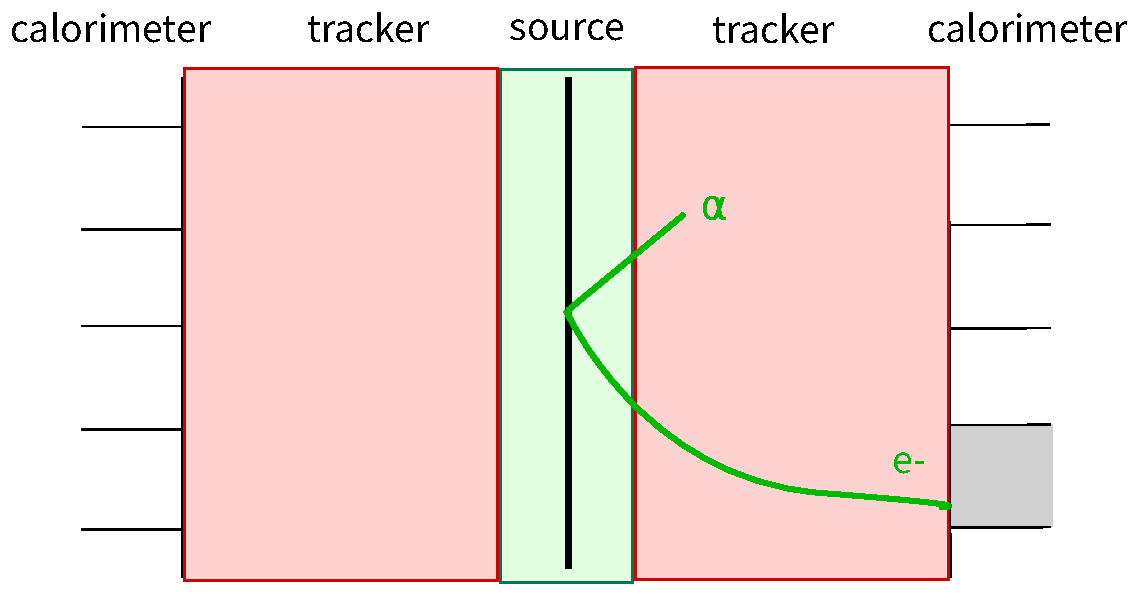
\includegraphics[scale=0.6]{pictures/Chap5/cartoon_source_selection.pdf}
\caption{Source selection diagram of the source selection. The green part represents the region where the events are selected.}
\label{cartoon_source_selection}
\end{center}
\end{figure}


\noindent The design of SuperNEMO has been optimized to detect electrons coming from the source foil. The distance between the source foil and the main calorimeter wall is 45~cm. The presence of a magnetic field curves the charged particles and allows for charge separation. An electron emitted from the source foil, can easily cross the 9 layers of the tracker and hit the calorimeter. To be identified as an electron, a particle must come from the source foil, hit the main calorimeter wall, and have a reconstructed track with a negative curvature. The cut flow for selecting the electrons coming from the surface of the foil is summarized in Table~\ref{Cutflowelectron}.


\begin{table}[h!]
\begin{center}
\begin{tabular}{l|c|c}
 & N & $\epsilon$ \\
\toprule
$\#$ of simulated electrons & 308 000 & \\
\hline
$\#$ of reconstructed electrons & 353 117 & 114.6 $\pm$ 0.2 \%\\
$\#$ coming from the foil       & 296 440 & 96.2  $\pm$ 0.2 \%\\
$\#$ hiting the main wall       & 126 520 & 41.1  $\pm$ 0.2 \%\\
$\#$ having a negative charge   & 116 325 & 37.8  $\pm$ 0.2 \%\\
\bottomrule
\end{tabular}
\end{center}
\caption{Cut flow of the electrons coming from the surface of the foil. The efficiencies are computed by dividing by the number of simulated electrons.}
\label{Cutflowelectron}
\end{table}


\bigskip


\noindent The number of reconstructed particles is higher than the number of simulated electrons (+114.6 $\pm$ 0.2\%). This is due to some events, where the number of reconstructed particles can be higher than 1. The number of reconstructed particles can reach 4 or 5 in some events. An electron can be scattered by a wire in the tracker or can rebound on a calorimeter wall. The track is broken. In this case, CAT recognizes two clusters. These two clusters are then processed independently by TrackFit which fits two tracks instead of only one. In the future, a specific module could be implemented to merge these events in a single particle. 


\bigskip


\noindent More than 96~\% of the reconstructed particles come from the source foil. 42.2$\pm$0.2\% of the particles possess both a vertex on the source foil and a calorimeter impact in the main wall. Finally, by requiring negative charge, selection efficiency drops to 38.8~$\pm$~0.2~$\%$.  The number of Geiger hits, the length of the track, and the energy of the electrons are shown in Figure~\ref{electron_gghit_length_time_energy_sss}.


\begin{figure}[h!]
\begin{center}
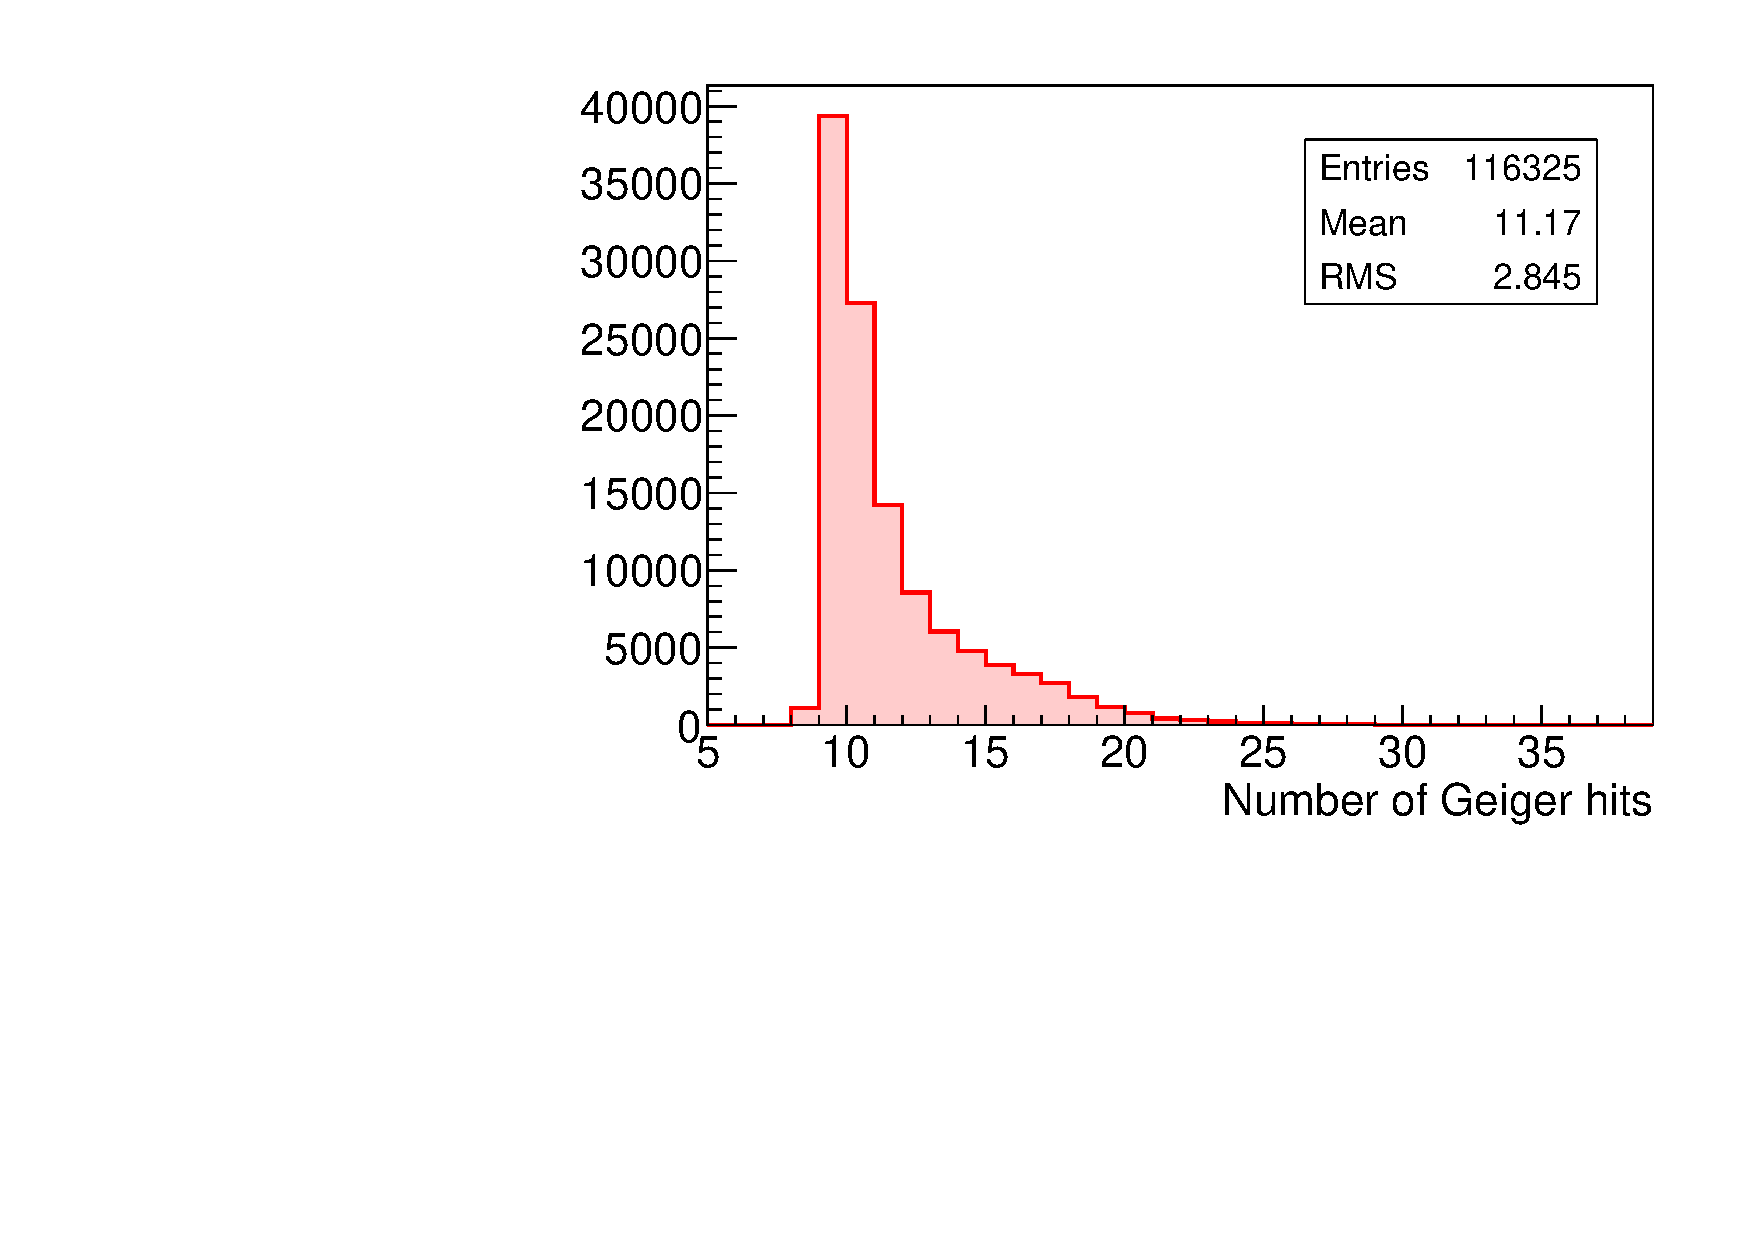
\includegraphics[scale=0.32]{pictures/Chap5/source_selection_surface_gghits.pdf}
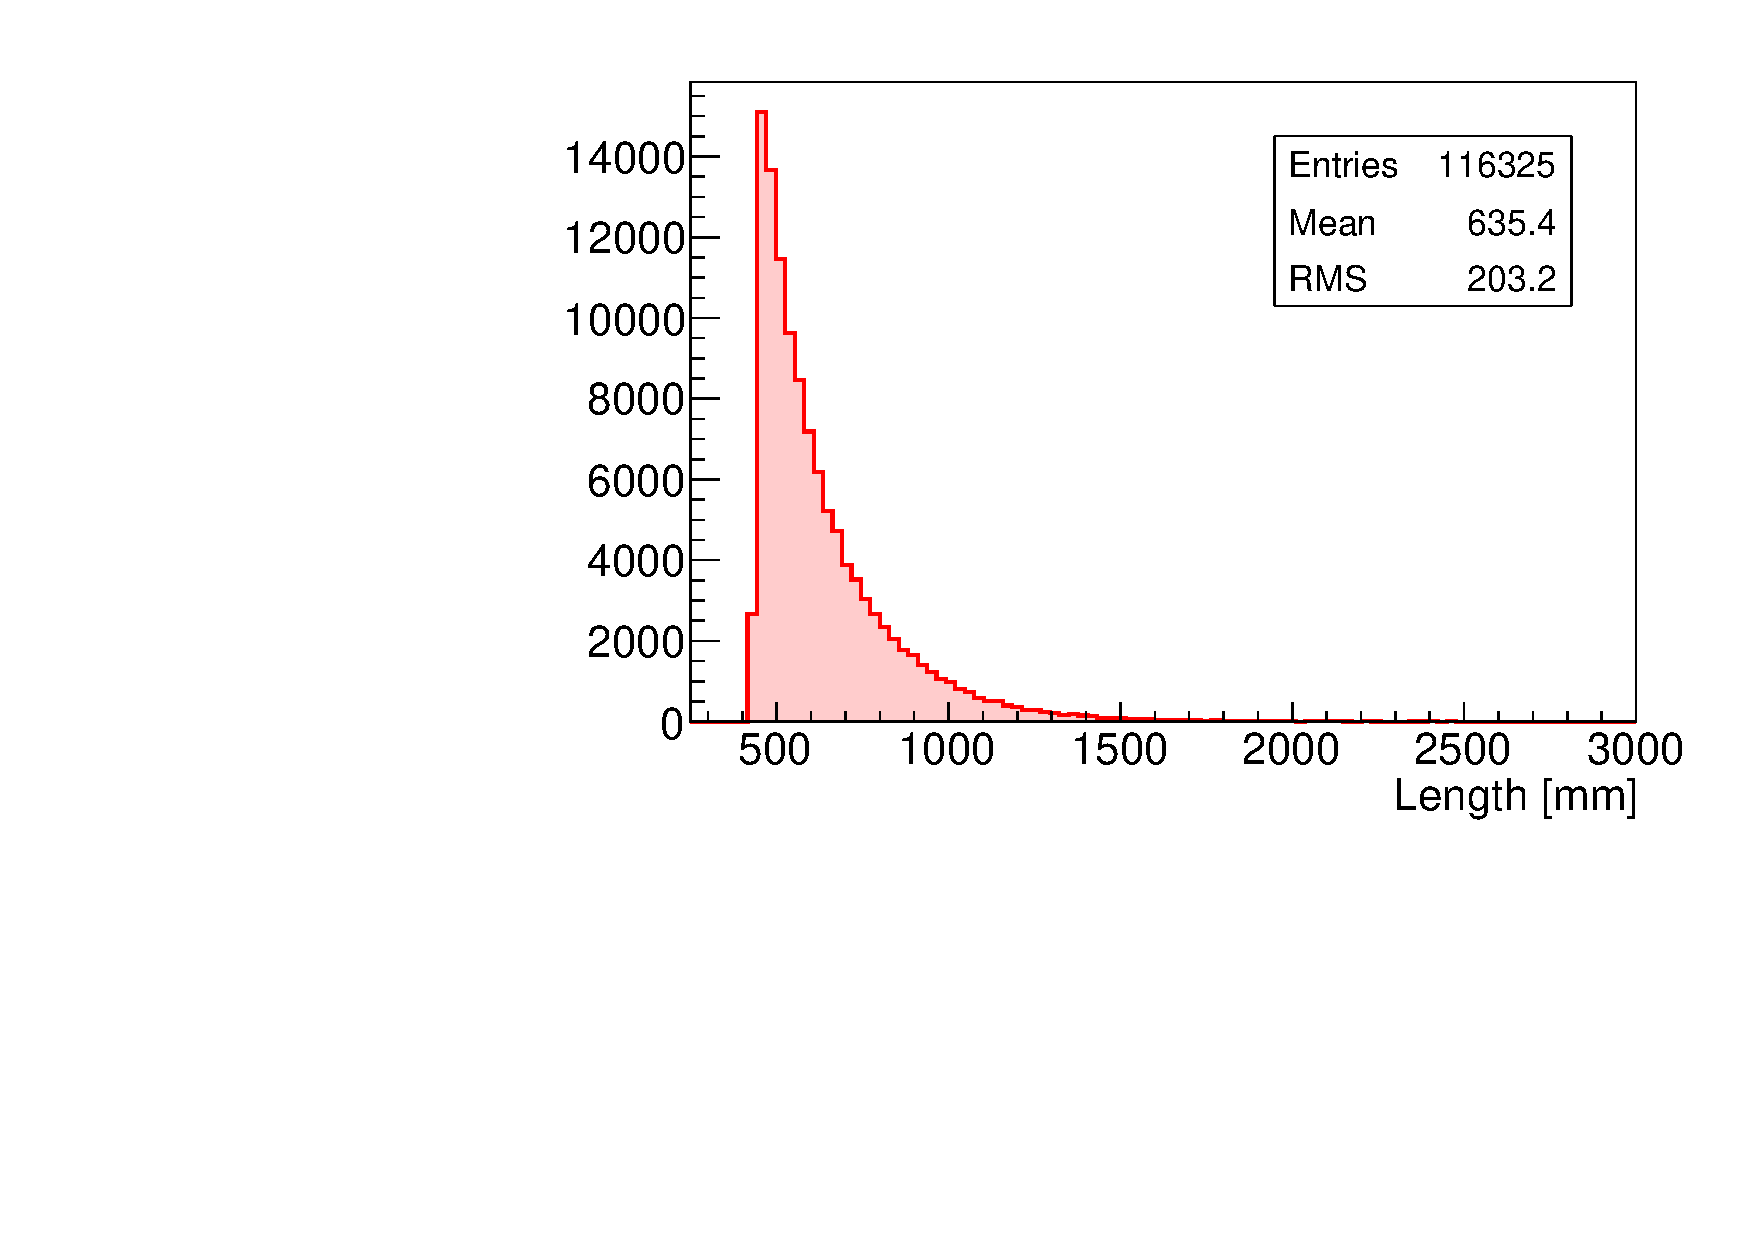
\includegraphics[scale=0.32]{pictures/Chap5/source_selection_surface_length.pdf}
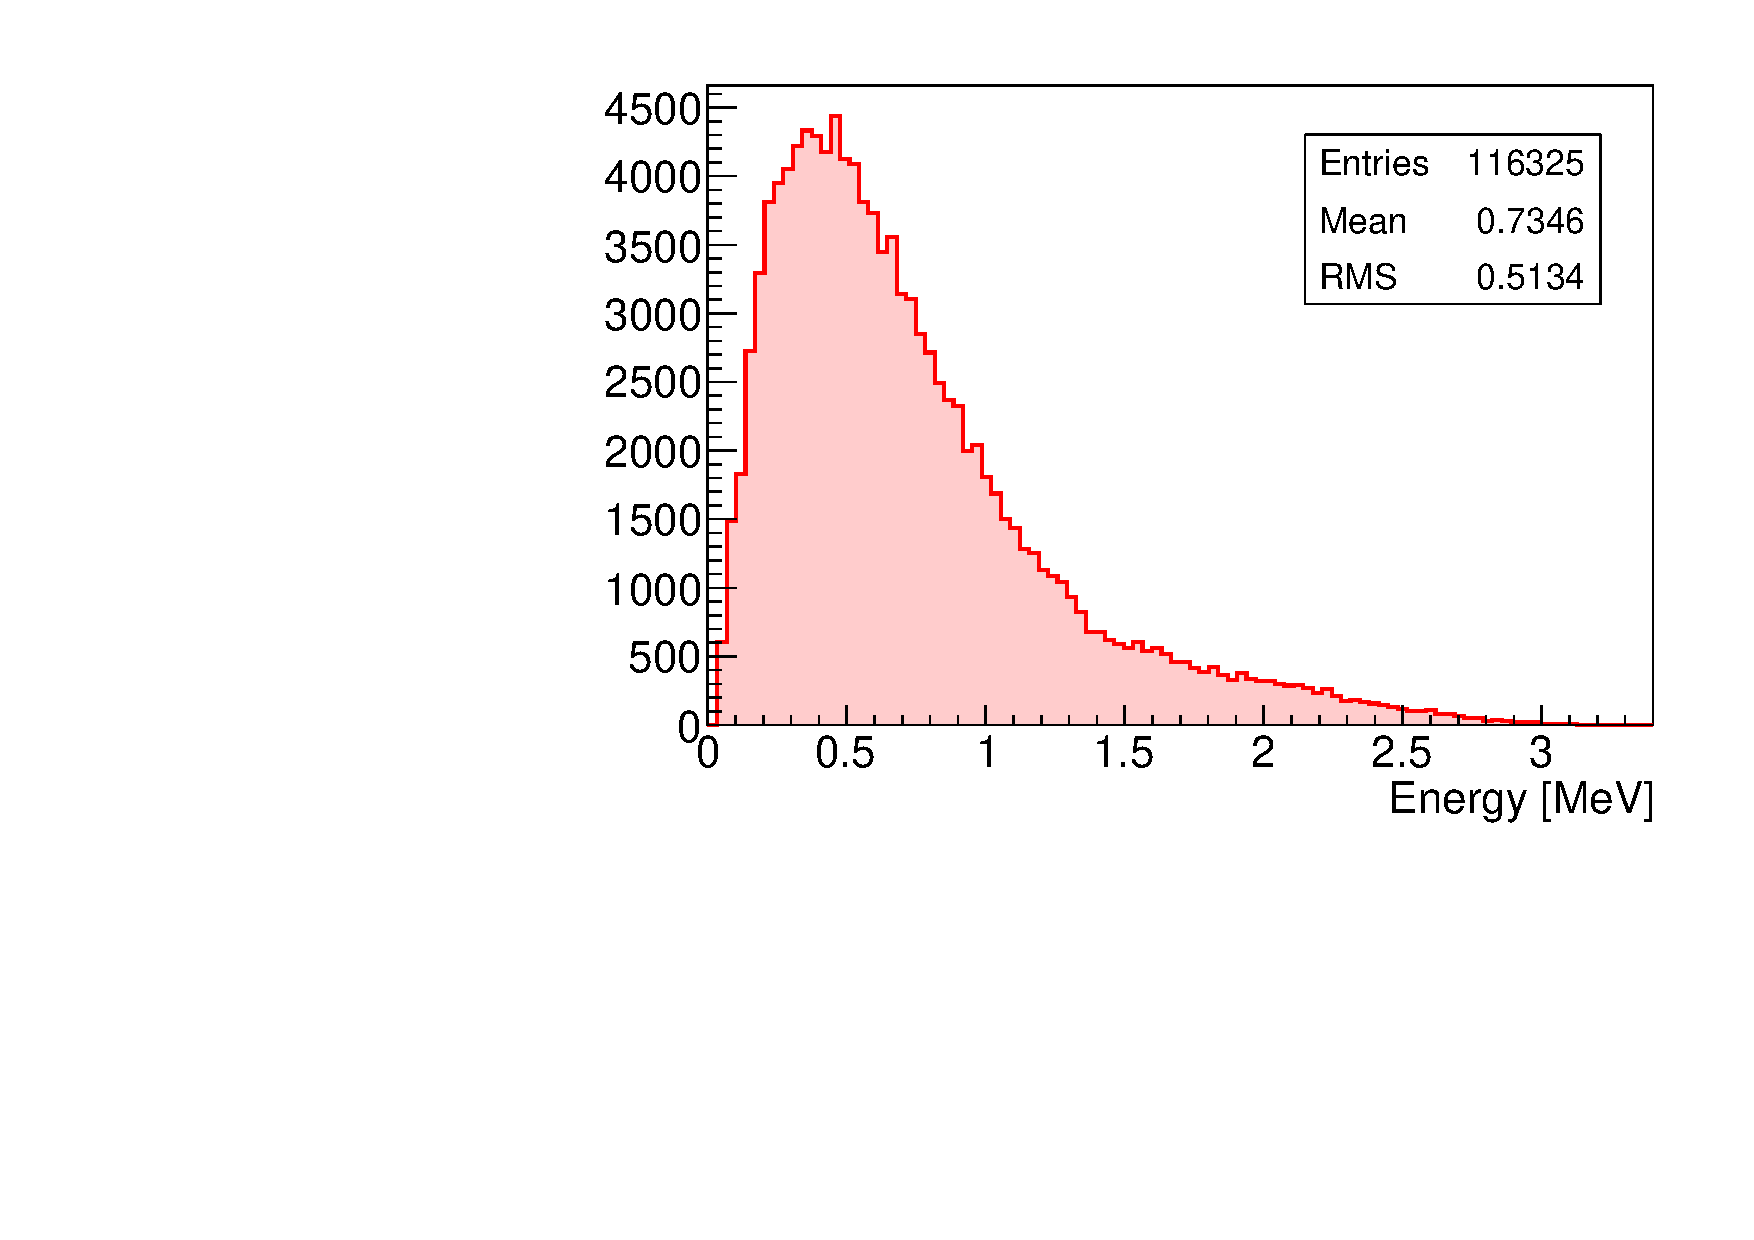
\includegraphics[scale=0.32]{pictures/Chap5/source_selection_surface_energy.pdf}
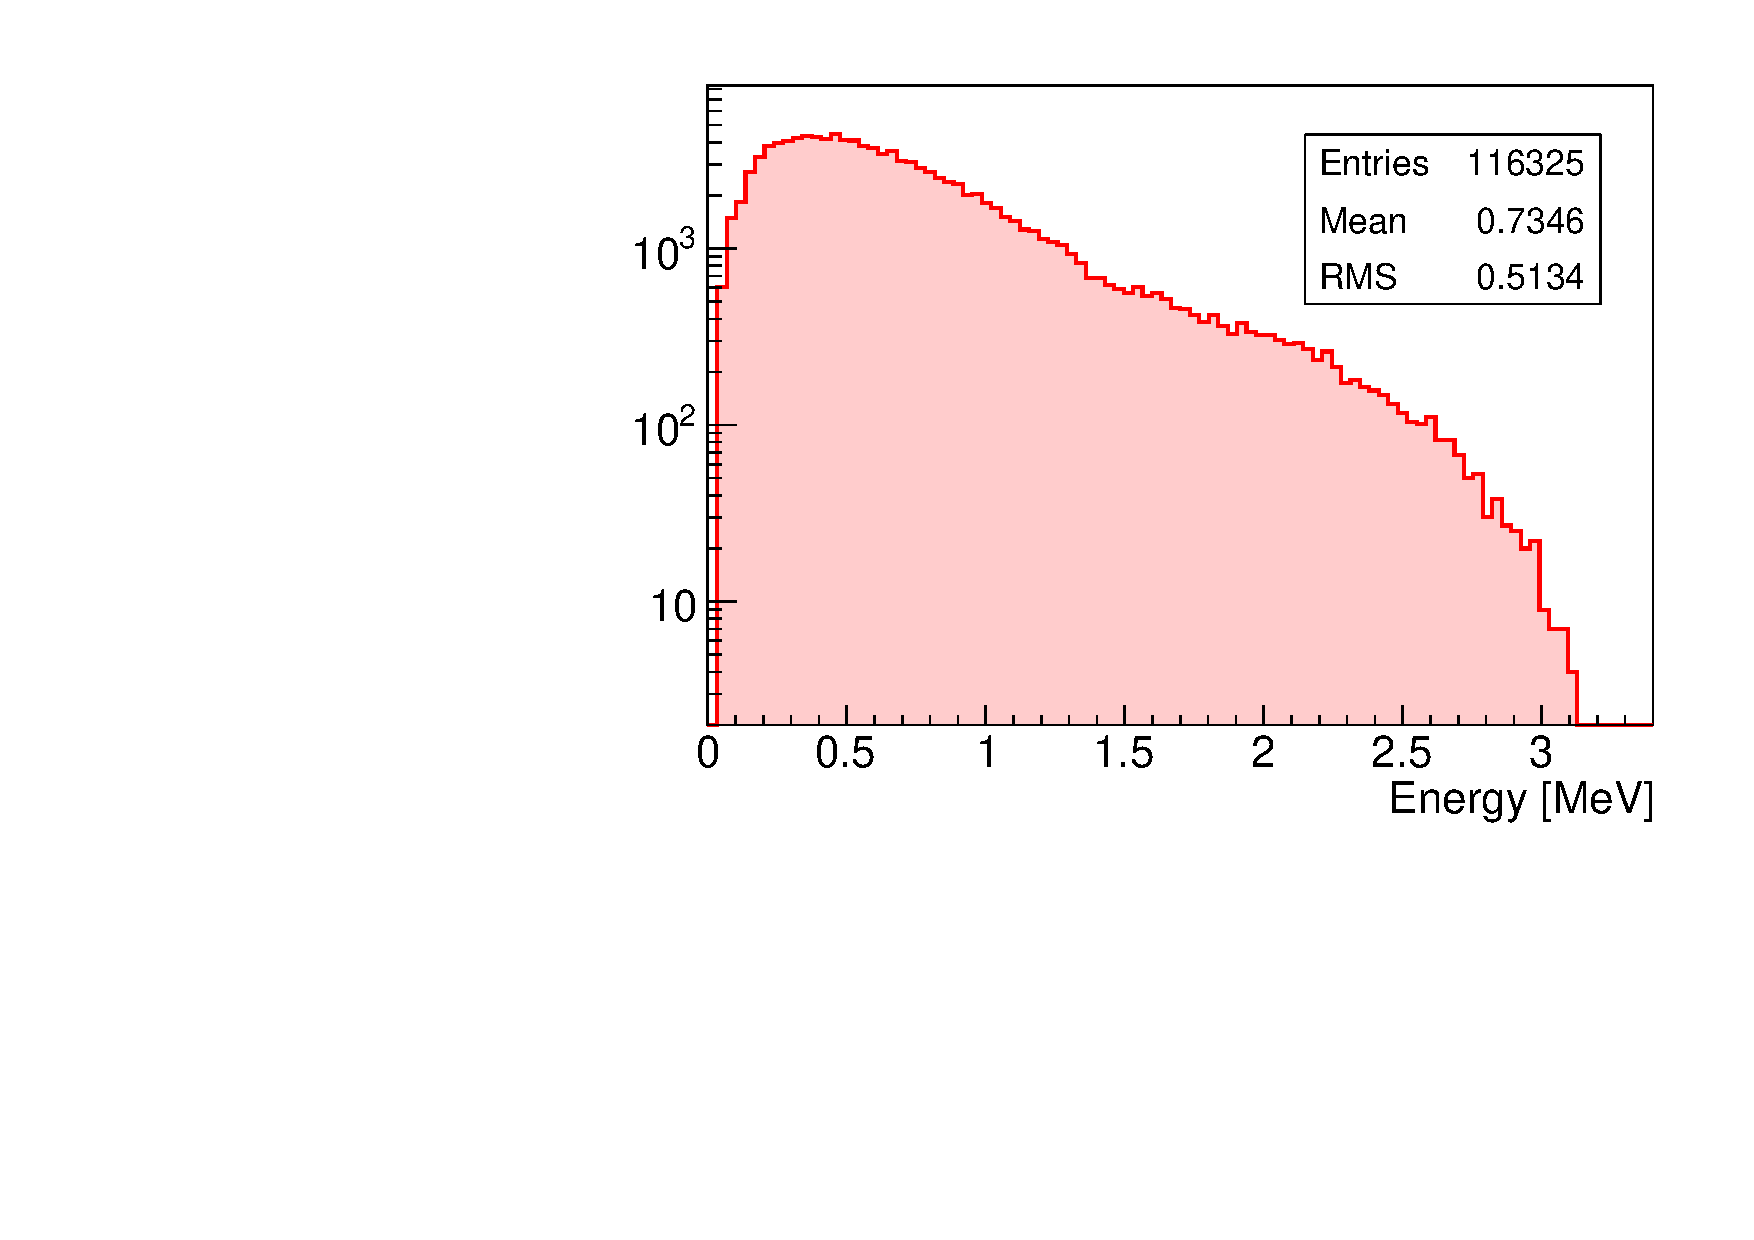
\includegraphics[scale=0.32]{pictures/Chap5/source_selection_surface_energy_log.pdf}
\caption{Top left : distribution of the number of Geiger hits for the electrons. Top right~: length of the selected electron tracks. Bottom left : energy spectrum of the selected electron. Bottom right : energy spectrum in log scale}
\label{electron_gghit_length_time_energy_sss}
\end{center}
\end{figure}


\bigskip


\noindent The number of Geiger hits is always greater than 8. This result makes sense because the tracker has 9 layers of wires between the source foil and the main calorimeter wall and the electron must cross the entire distance. Similarly, the distance between the source foil and the main calorimeter wall is 45 cm, so the minimum length observed cannot be smaller than this distance. The mean distance travelled by an electron is 63 cm. The energy spectrum looks like the expected energy spectrum of the  $^{\text{214}}$Bi with the Q-value of 3.27 MeV.


\bigskip


\noindent The cut flow of the electrons coming from the bulk of the foil and coming from the tracker are summarized in Table~\ref{Cutflowelectronbulk} and Table~\ref{Cutflowelectrontrackercomingfromthesource}.


\begin{table}[h!]
\begin{center}
\begin{tabular}{l|c|c}
 & N & $\epsilon$ \\
\toprule
$\#$ of simulated electrons & 308 000 & \\
\hline
$\#$ of reconstructed electrons & 320 379 & 104.0 $\pm$ 0.2 \% \\
$\#$ coming from the foil       & 272 325 & 88.4  $\pm$ 0.2 \% \\
$\#$ hiting the main wall       & 133 255 & 43.3  $\pm$ 0.2 \% \\
$\#$ having a negative charge   & 122 170 & 39.7  $\pm$ 0.2 \% \\
\bottomrule
\end{tabular}
\end{center}
\caption{Cut flow of the electrons coming from the bulk of the foil. The efficiencies are computed by dividing by the number of simulated electrons.}
\label{Cutflowelectronbulk}
\end{table}



\begin{table}[h!]
\begin{center}
\begin{tabular}{l|c|c}
 & N & $\epsilon$ \\
\toprule
$\#$ of simulated electrons & 308 000 & \\
\hline
$\#$ of reconstructed electrons & 385 176 & 125.0 $\pm$ 0.2 \% \\
$\#$ coming from the foil       & 210 811 & 68.4  $\pm$ 0.2 \%\\
$\#$ hiting the main wall       & 60 279  & 19.6  $\pm$ 0.2 \%\\
$\#$ having a negative charge   & 51 480  & 16.7  $\pm$ 0.2 \%\\
\bottomrule
\end{tabular}
\end{center}
\caption{Cut flow of the electrons coming from the tracker. The efficiencies are computed by dividing by the number of simulated electrons.}
\label{Cutflowelectrontrackercomingfromthesource}
\end{table}


\bigskip


\noindent With the source selection, $\sim$ 17 \% of the electrons generated in the tracker are reconstructed and selected. These electrons correspond to events where the electron is simulated on the first layer close to the source foil. The vertex of these events is extrapolated and is considered to be on the source foil.


\bigskip


\noindent In order to verify the usefulness and the influence of the charge cut, a study is realized. The definition of the charge confusion is introduced as the ratio between the number of true electrons that have been reconstructed with a positive or no charge over the total of true electrons.


\begin{equation}
\text{charge confusion} = \frac{N_e^{\text{wrong}}}{N_e^{\text{tot}}}
\end{equation}     


\bigskip


\noindent Figure~\ref{charge_confusion_source_plots} (left) shows the electron track length. The black curve represents all the reconstructed electrons coming from the foil and hitting the main wall. The fraction of these electrons reconstructed with a negative charge are shown in red. The electrons reconstructed with a positive or no charge are plotted in blue. Figure~\ref{charge_confusion_source_plots} (right) also shows the charge confusion with respect to the length of the electron track. 

\bigskip


\begin{figure}[h!]
\begin{center}
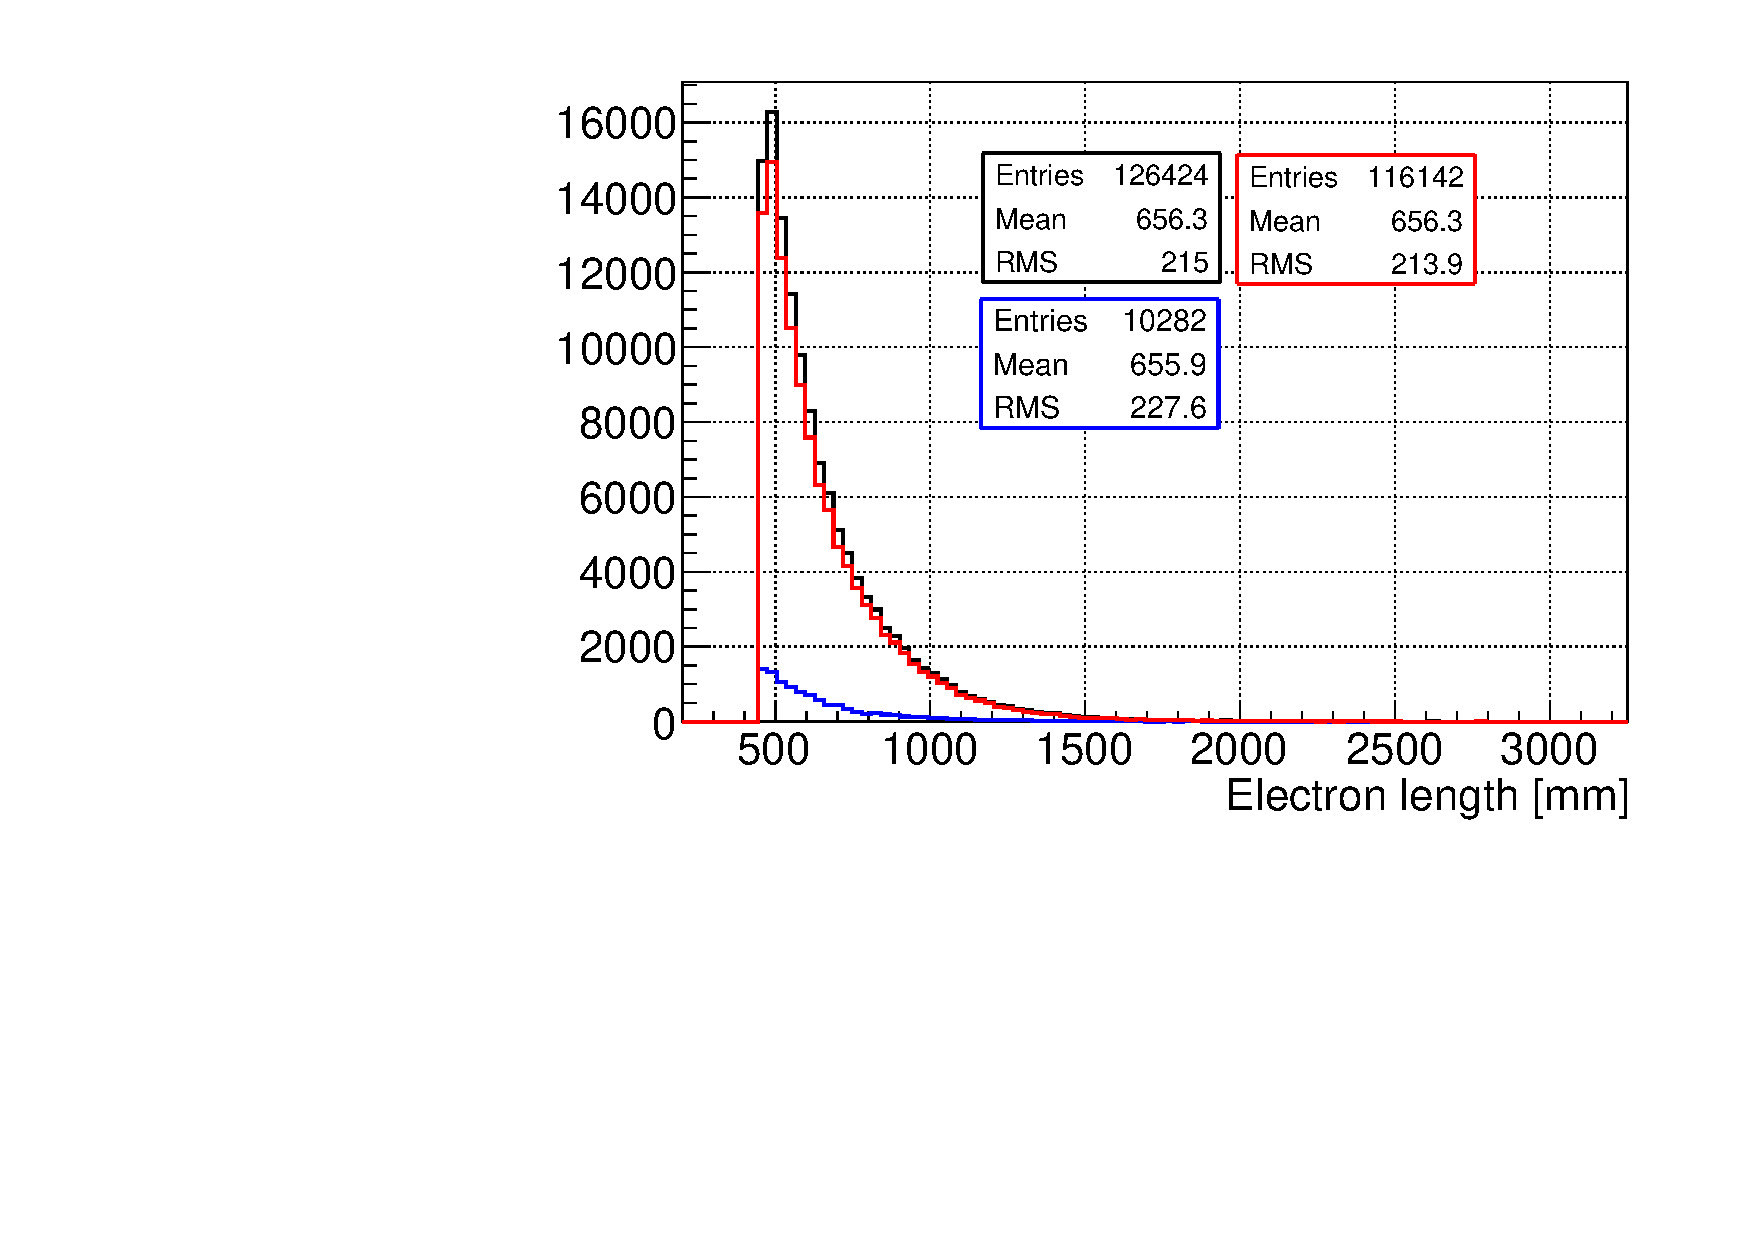
\includegraphics[scale=0.34]{pictures/Chap5/length_source_charge_confusion_2.pdf}
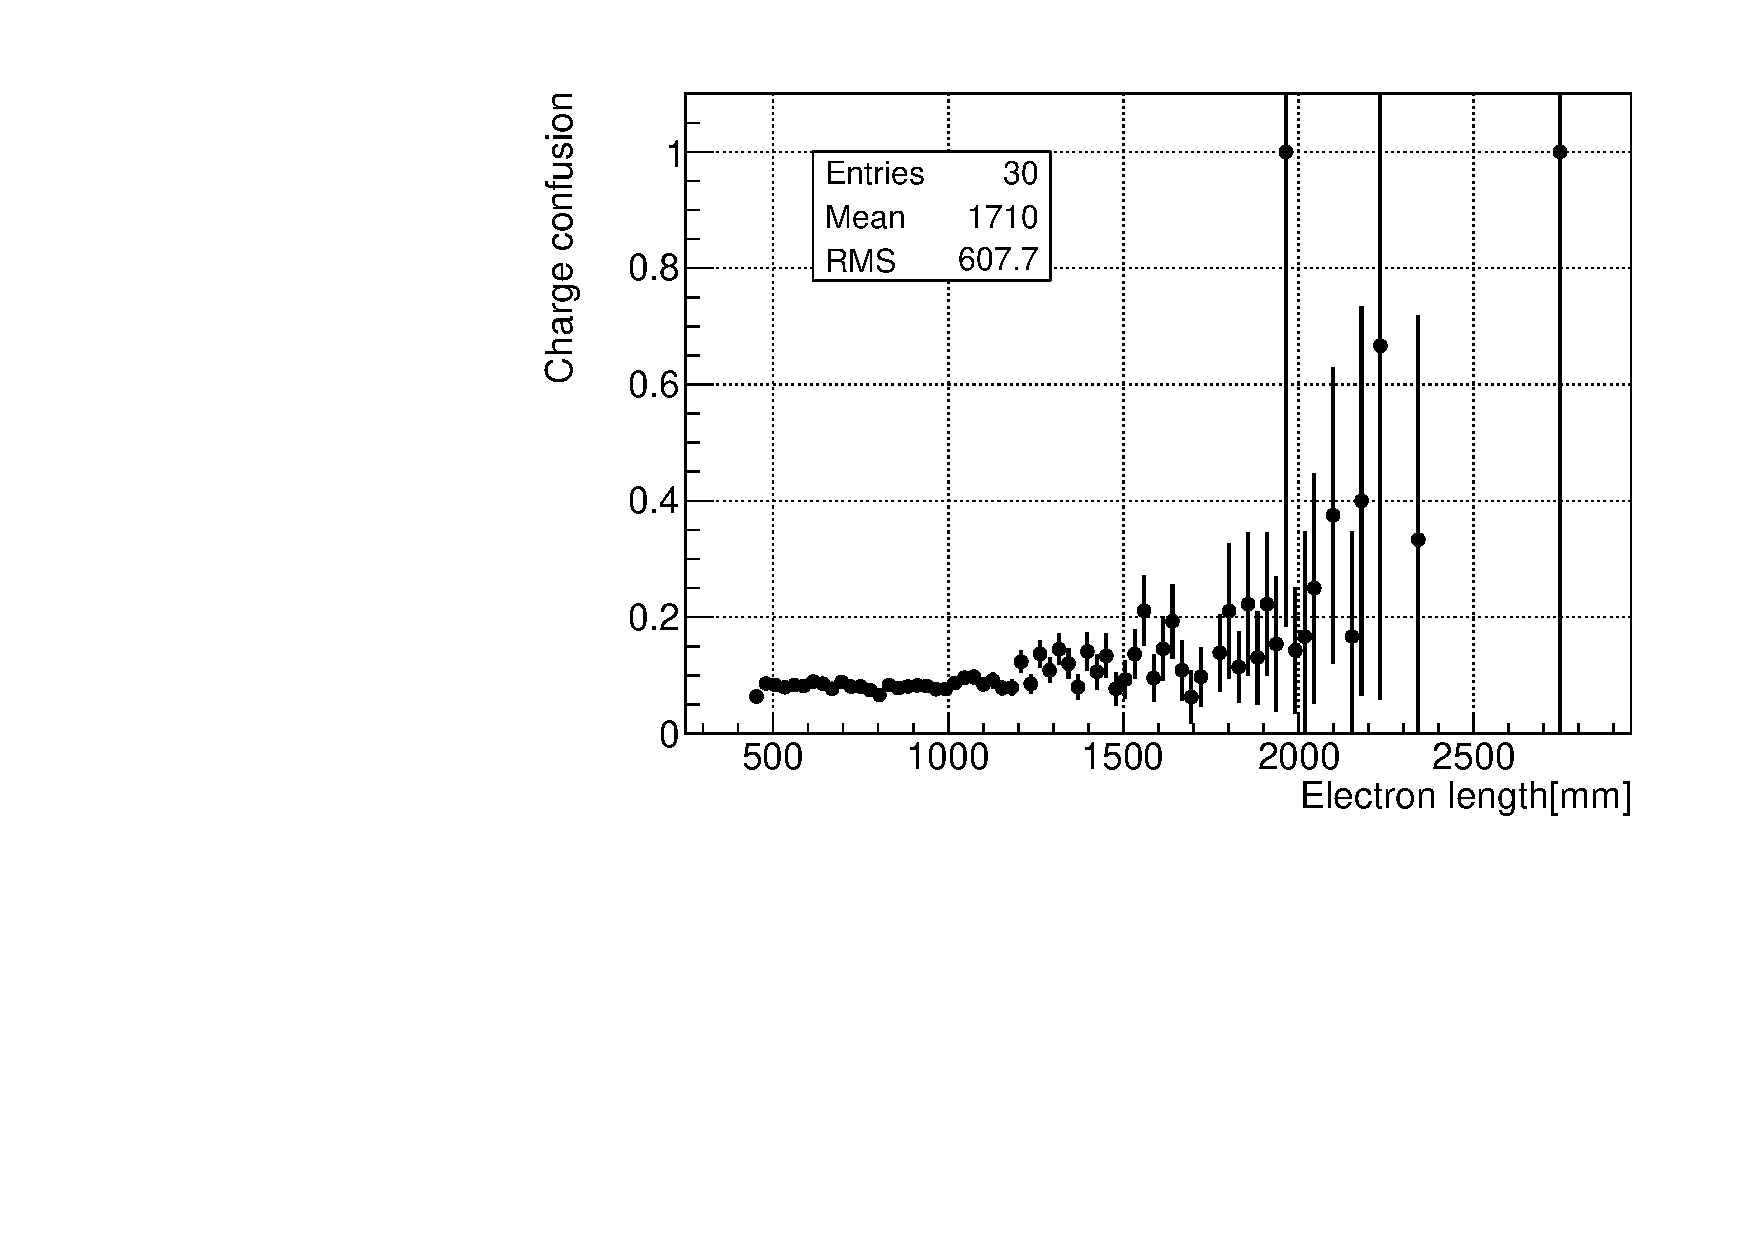
\includegraphics[scale=0.34]{pictures/Chap5/charge_confusion_length_source.pdf}
\caption{On the left : length of the electron track for different charge. The black curve represents all the reconstructed electrons coming from the foil and hitting the main wall. In red, the electrons coming from the source foil and hitting the main wall reconstructed with a negative charge. In blue, the electrons reconstructed with a positive or undefined charge. On the right: the charge confusion vs the length of the electron track.}
\label{charge_confusion_source_plots}
\end{center}
\end{figure}


\bigskip


\noindent For the events coming from the source foil, the charge confusion is $\sim$ 8 $\%$ and remains constant as a function of the length of the electron track. This criteria on the charge suppresses the multi-scattering of the electron inside the tracker chamber. For the selection of 1e1$\alpha$ events coming from the source foil, this charge cut is used in order to get a high purity electron sample.


\FloatBarrier


\noindent To be identified as an alpha, the particle must be delayed, coming from the source foil without hitting the calorimeter. The cut flow of the alpha coming from the surface of the source foil is shown in Table~\ref{Cutflowelectronalpha}.


\begin{table}[h!]
\begin{center}
\begin{tabular}{l|c|c}
 & N & $\epsilon$ \\
\hline
$\#$ of simulated alphas & 300 000 & \\
\hline
$\#$ of reconstructed alpha & 104 288 & 34.8 $\pm$ 0.2\%\\
$\#$ being delayed          & 104 288 & 34.8 $\pm$ 0.2\%\\
$\#$ coming from the foil   & 87 316  & 29.1 $\pm$ 0.2\%\\
$\#$ not hitting the calorimeter & 87 316  & 29.1 $\pm$ 0.2\%\\
\end{tabular}
\end{center}
\caption{Cut flow of the alpha coming from the foil surface. The efficiencies are computed by dividing by the number of simulated alphas.}
\label{Cutflowelectronalpha}
\end{table}


\bigskip


\noindent After the simulation, 34.8~\% of the alpha particles are reconstructed. Compared to the electron detection efficiency this number is much lower. Due to the high energy losses, events generated towards the source foil will not cross it, and $\sim$50~\% of the events are lost. The number of alpha particles found by our criteria is 29.2~$\pm$~0.2~\% of the simulated particle. The length and the number of Geiger hits of the alpha particles are plotted in Figure \ref{alphaLengthSSS}.


\bigskip


\begin{figure}[h!]
\begin{center}
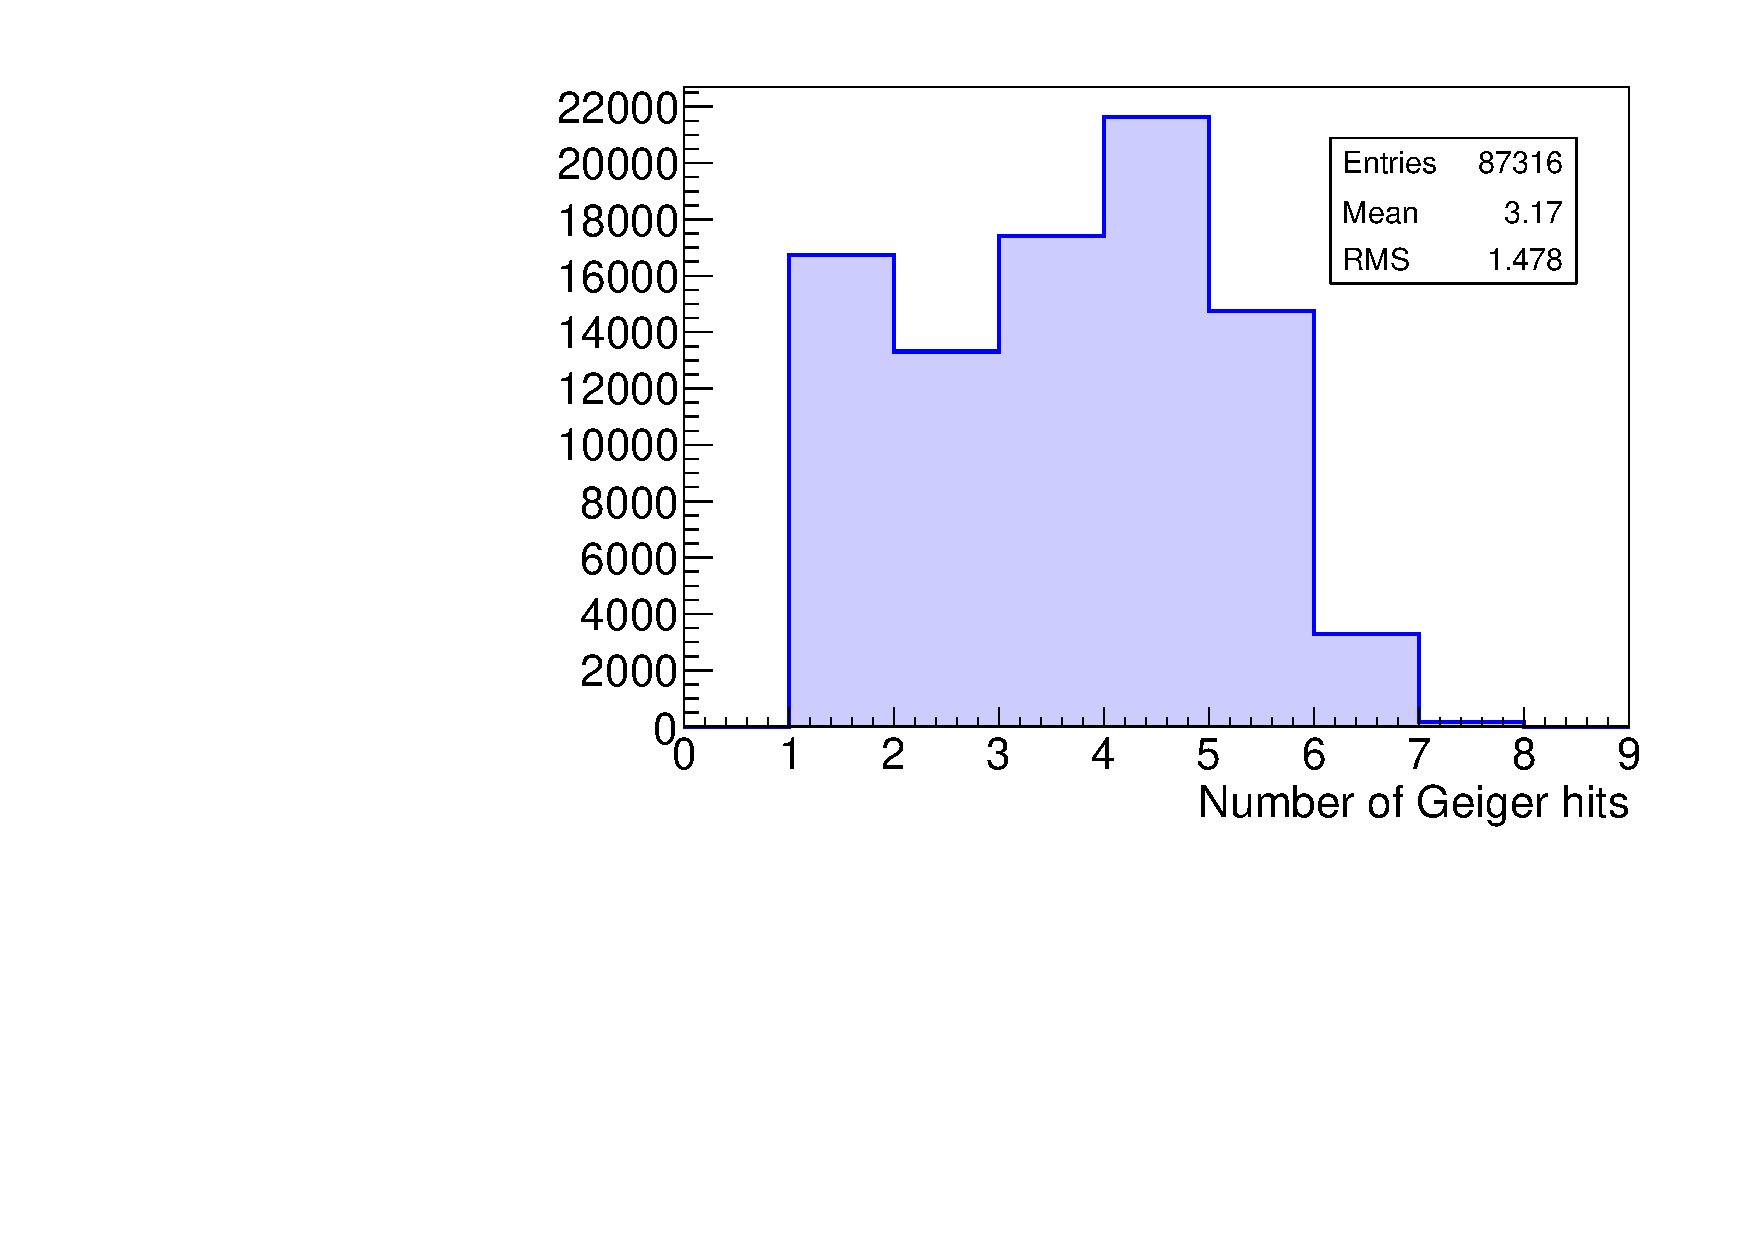
\includegraphics[scale=0.33]{pictures/Chap5/source_selection_surface_gghits_alpha.pdf}
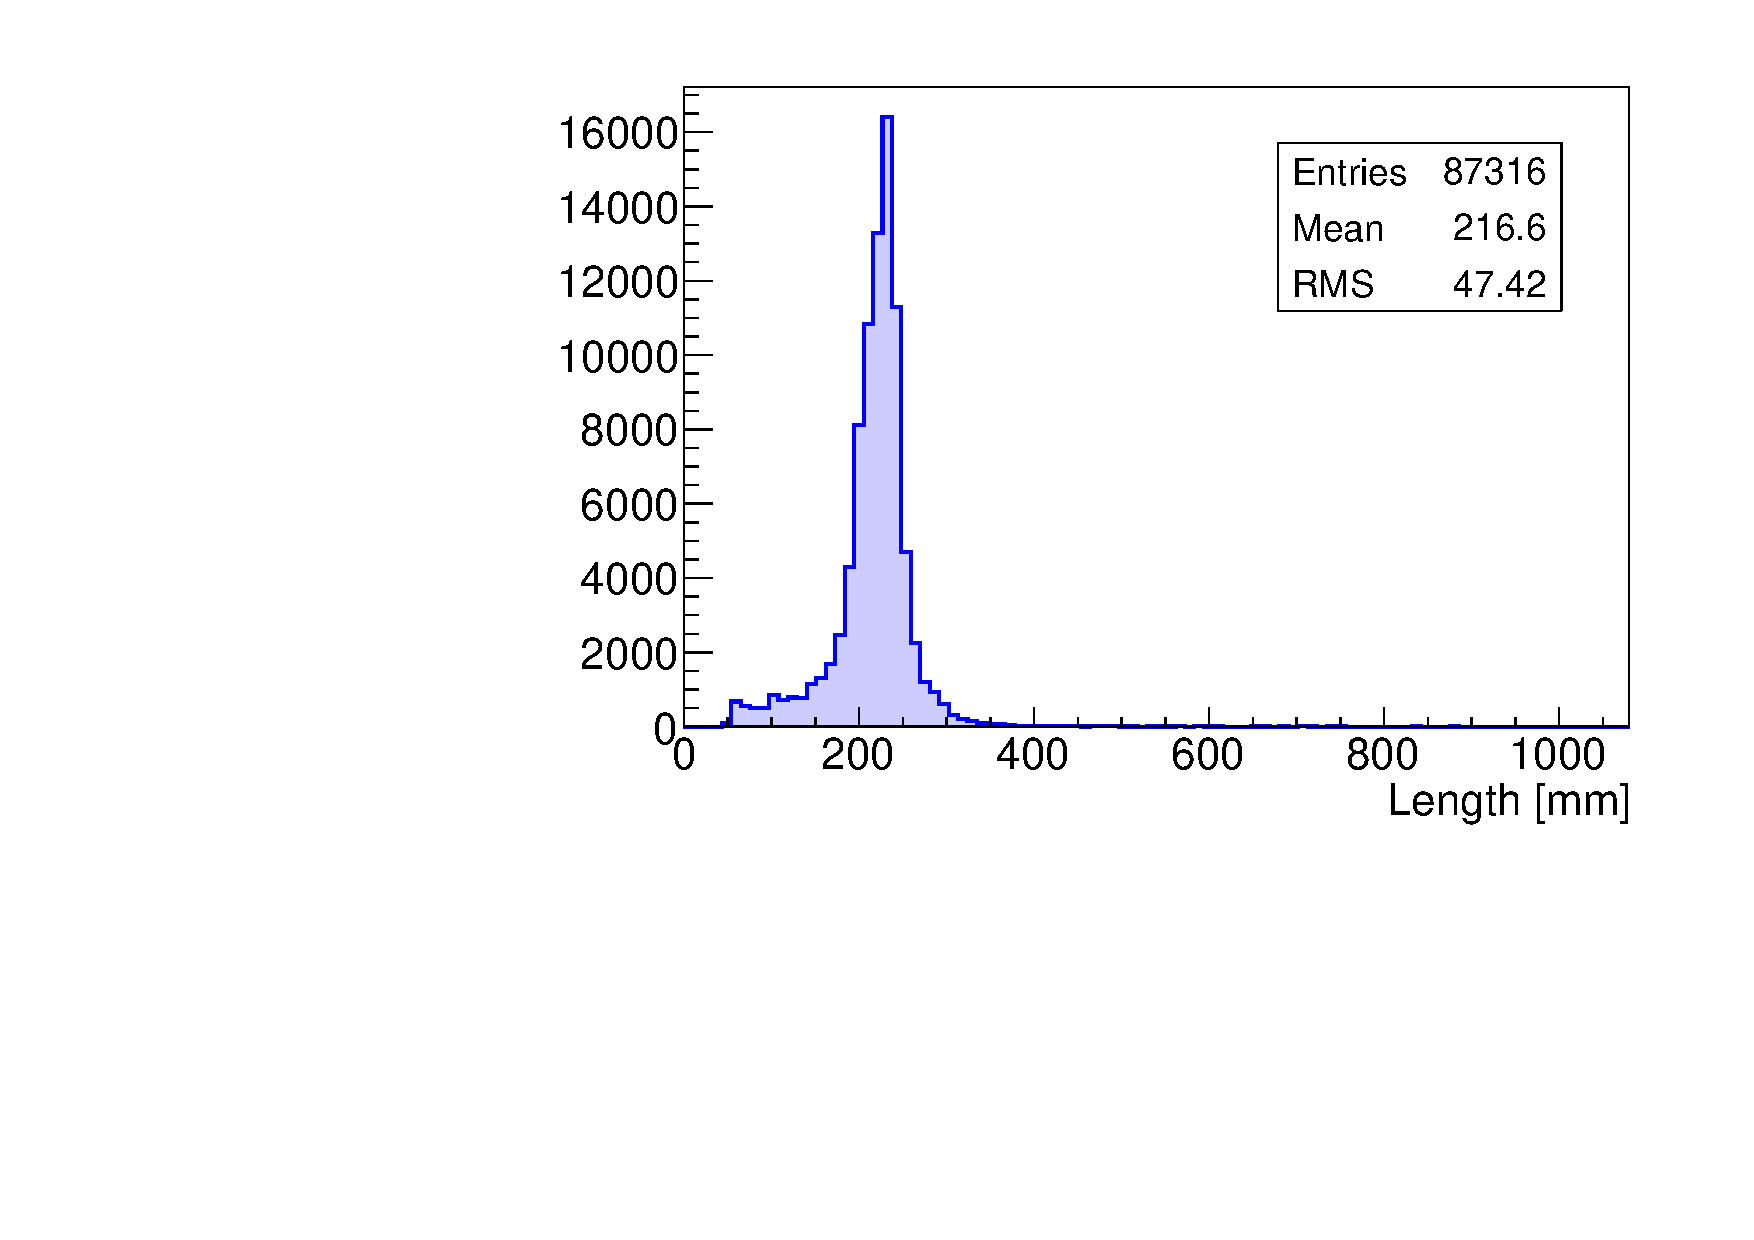
\includegraphics[scale=0.33]{pictures/Chap5/source_selection_surface_length_alpha.pdf}
\caption{$(a)$ On the left, the number of Geiger hits for the alpha particles. On the right the length of the track of the alphas}
\label{alphaLengthSSS}
\end{center}
\end{figure}


\noindent As expected the number of Geiger hits is low and does not exceed 9. The average number of Geiger hits for an alpha particle is 4. The mean track length of the identified alpha is $\sim$22 cm which is consistent with the estimated value in section~4, knowing that the tracker gas is made of 95~\% of He. The cut flow of the alphas coming from the bulk of the foil and coming from the tracker are presented in Table~\ref{Cutflowalphabulk} and Table~\ref{Cutflowalphatrackerselection} respectively. 


\begin{table}[h!]
\begin{center}
\begin{tabular}{l|c|c}
 & N & $\epsilon$ \\
\toprule
$\#$ of simulated alphas & 300 000 & \\
\hline
$\#$ of reconstructed alpha & 33 876 & 11.3 $\pm$ 0.2\% \\
$\#$ being delayed          & 33 876 & 11.3 $\pm$ 0.2\% \\
$\#$ coming from the foil   & 24 306 & 8.1  $\pm$ 0.2\% \\
$\#$ not hitting the calorimeter & 24 301 & 8.1  $\pm$ 0.2\% \\
\bottomrule
\end{tabular}
\end{center}
\caption{Cut flow of the alpha coming from the foil bulk. The efficiencies are computed by dividing by the number of simulated alphas.}
\label{Cutflowalphabulk}
\end{table}


\begin{table}[h!]
\begin{center}
\begin{tabular}{l|c|c}
 & N & $\epsilon$ \\
\toprule
$\#$ of simulated alphas & 300 000 & \\
\hline
$\#$ of reconstructed alpha & 131 596 & 43.9 $\pm$ 0.2\% \\
$\#$ being delayed          & 131 596 & 43.9 $\pm$ 0.2\% \\
$\#$ coming from the foil   & 32 737  & 10.9 $\pm$ 0.2\% \\
$\#$ not hitting the calorimeter & 32 716  & 10.9 $\pm$ 0.2\% \\
\bottomrule
\end{tabular}
\end{center}
\caption{Cut flow of the alpha coming from the tracker. The efficiencies are computed by dividing by the number of simulated alphas.}
\label{Cutflowalphatrackerselection}
\end{table}


\bigskip


\noindent The 1e1$\alpha$ topology is built by associating, an electron and a delayed alpha. The track length of the alpha and the time between the electrons and the alphas are the main observables of this topology. The track length of the alphas according to the vertex generation (bulk in black, surface in blue, tracker in red) is shown in Figure~\ref{alpha_length_source_selection}.


\begin{figure}[h!]
\begin{center}
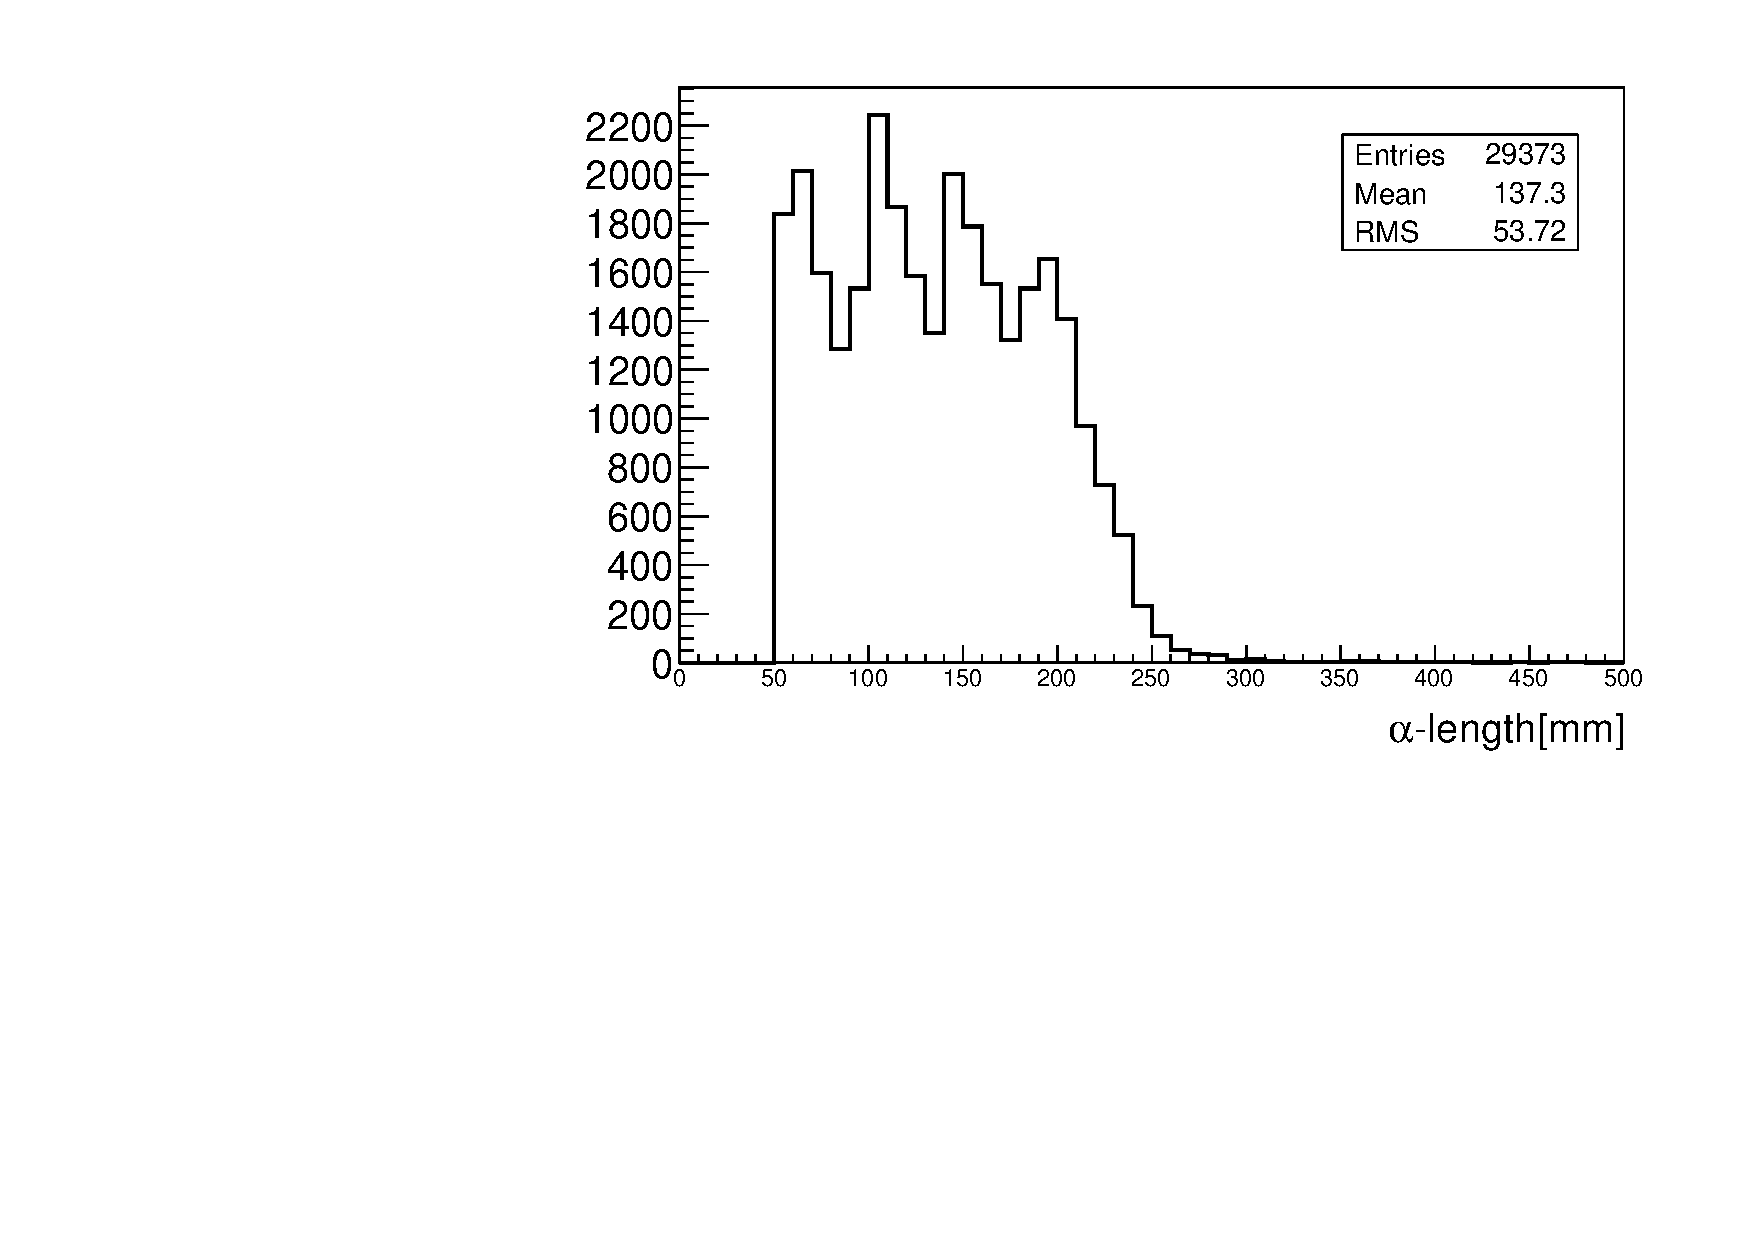
\includegraphics[scale=0.39]{pictures/Chap5/alpha_length_bulk_1M.pdf}
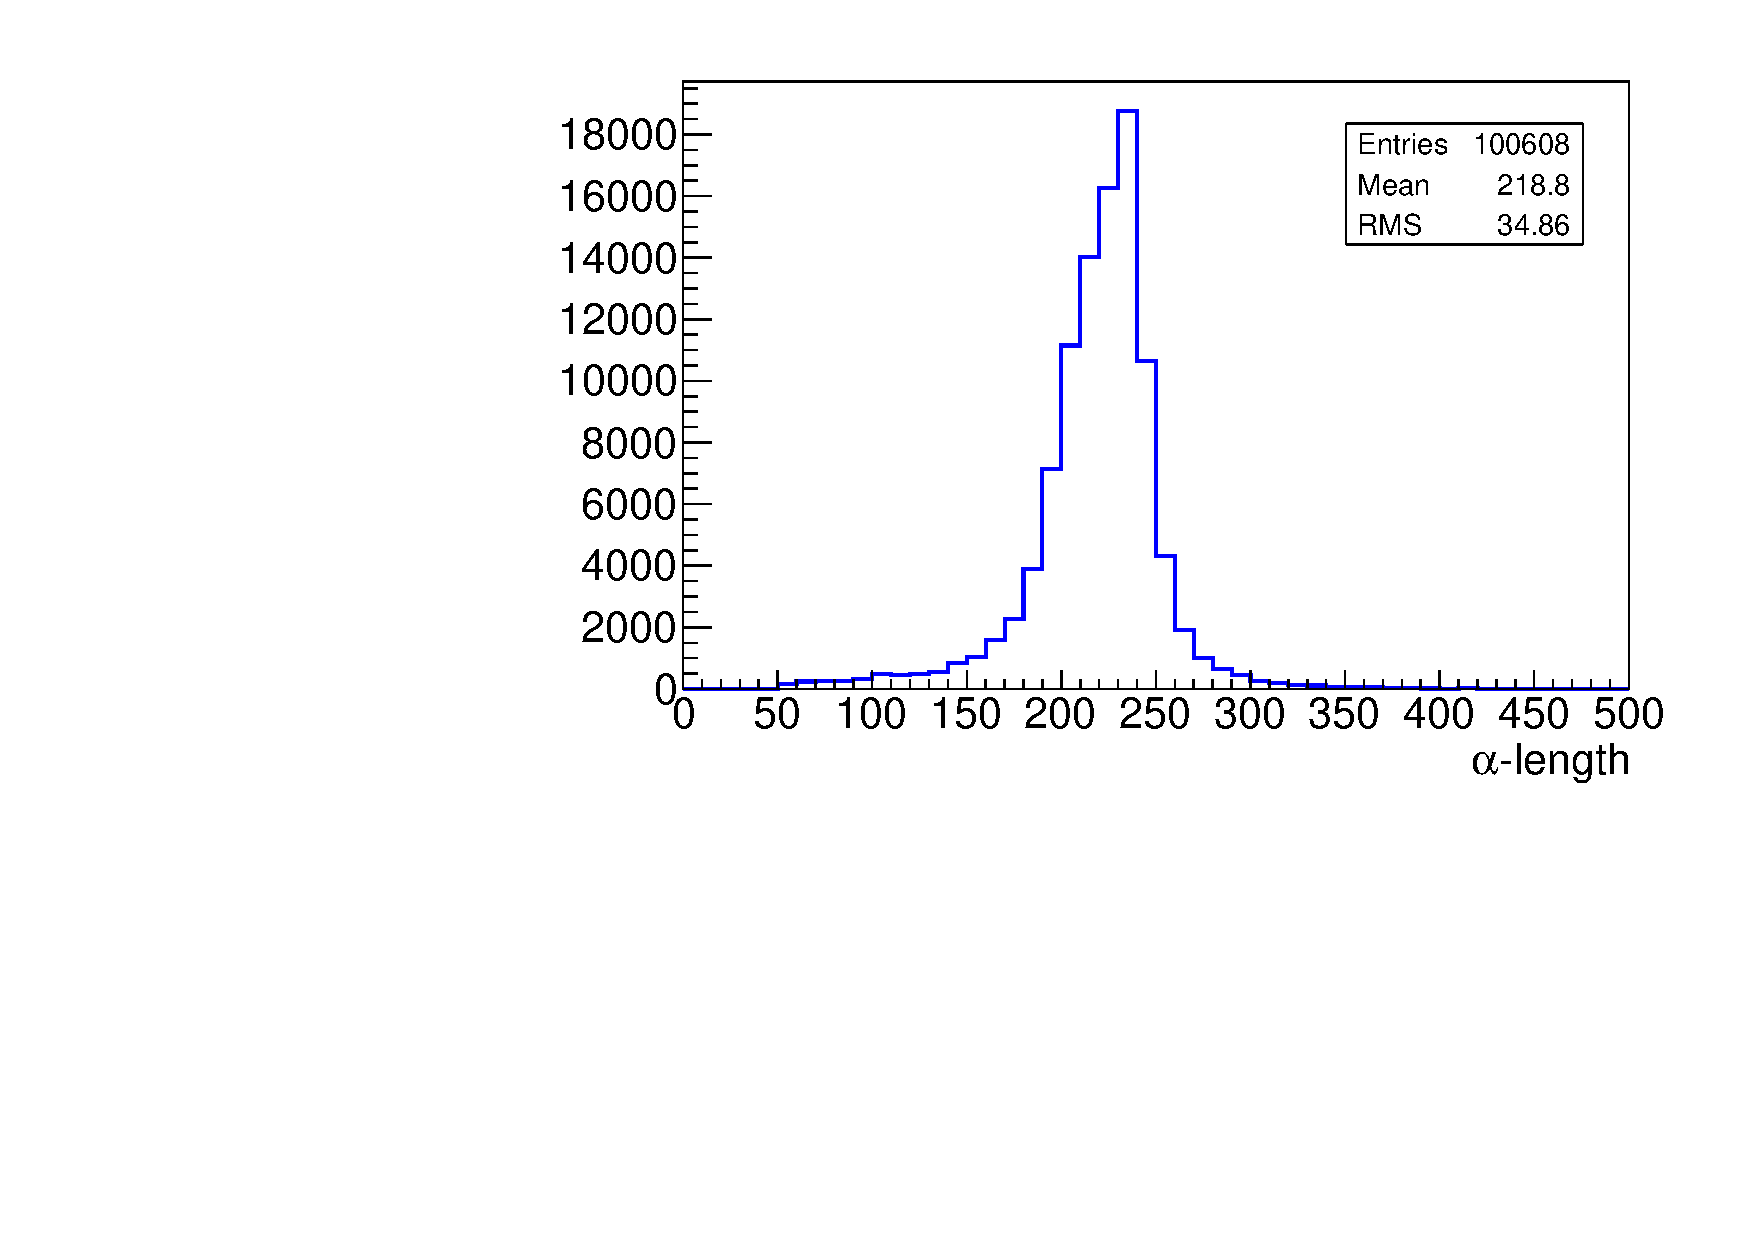
\includegraphics[scale=0.39]{pictures/Chap5/alpha_length_surface_1M.pdf}
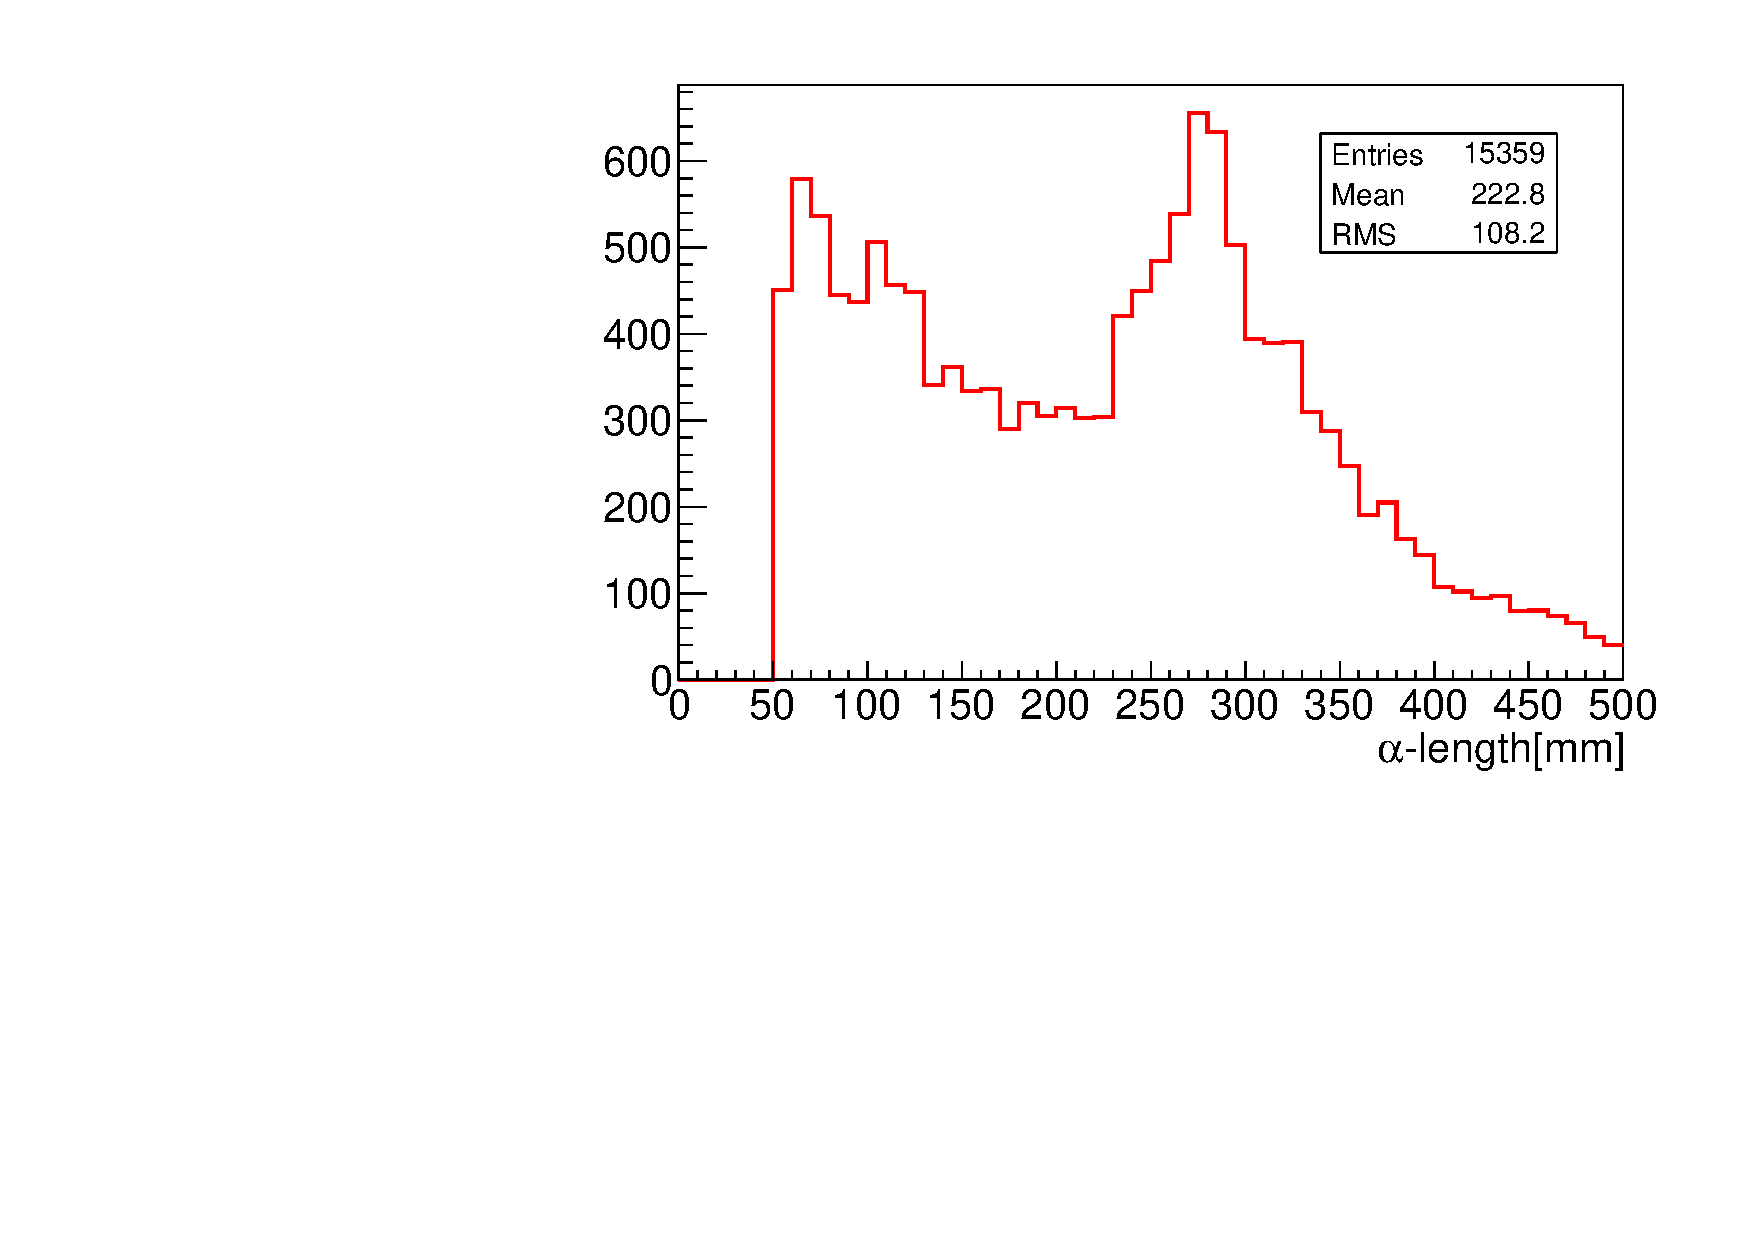
\includegraphics[scale=0.39]{pictures/Chap5/alpha_length_tracker_1M.pdf}
\caption{Alpha track length in the 1a1$\alpha$ channel. Top : events coming from the bulk. Middle : events coming from the surface of the foil. Bottom : events coming from the tracker.}
\label{alpha_length_source_selection}
\end{center}
\end{figure}


\FloatBarrier


\noindent Given the high ionisation power of the alpha particles, they lose a lot of energy just by crossing the source foil. Thus, the alpha particles coming from the bulk are expected to have a shorter track length than the alpha particles coming from the surface of the foil. The alpha particles coming from the tracker cross only the helium gas of the detector. Given the energy loss of the alpha in helium, the maximum length of the track will be around 45-50 cm.

\bigskip

\noindent The multi-peak distribution of the alpha particles coming from the bulk of the foil can be explained by the tracker configuration. The first peak corresponds to the alpha hitting the first tracker layer. The width of each peak corresponds to all the possible incident angles. The second peak corresponds to the alpha hitting the second layer of the tracker. This distribution is quite different from the distribution observed for the NEMO-3 experiment, due to the larger amount of wires in the tracker chamber which give us a better resolution on the length of the alpha. 
 %Figure~\ref{alpha_track_length_bulk_3D} represents the length of the alpha according the number of Geiger hits of the alpha.

%\begin{figure}[h!]
%\begin{center}
%\includegraphics[scale=0.42]
%{/home/lenoblet-local/Documents/Presentations/my_presentations/radon_work/2D_length_number_of_gg_hits_bulk.pdf}
%\caption{Distribution of the alpha track length coming from the bulk of the foil according to the number of Geiger hits}
%\label{alpha_track_length_bulk_3D}
%\end{center}
%\end{figure}


\bigskip


\noindent The delayed time between the electron and the alpha is plotted in Figure~\ref{delayedtimetopology}. The half-life of the process is found to be t$_{\text{1/2}}$ = 162.6 $\pm$ 4.1 $\mu s$. This agrees well with the published value of 164.6 $\pm$ 0.3 $\mu$s from~\cite{NuclearDataSheet210}.


\begin{figure}[h!]
\begin{center}
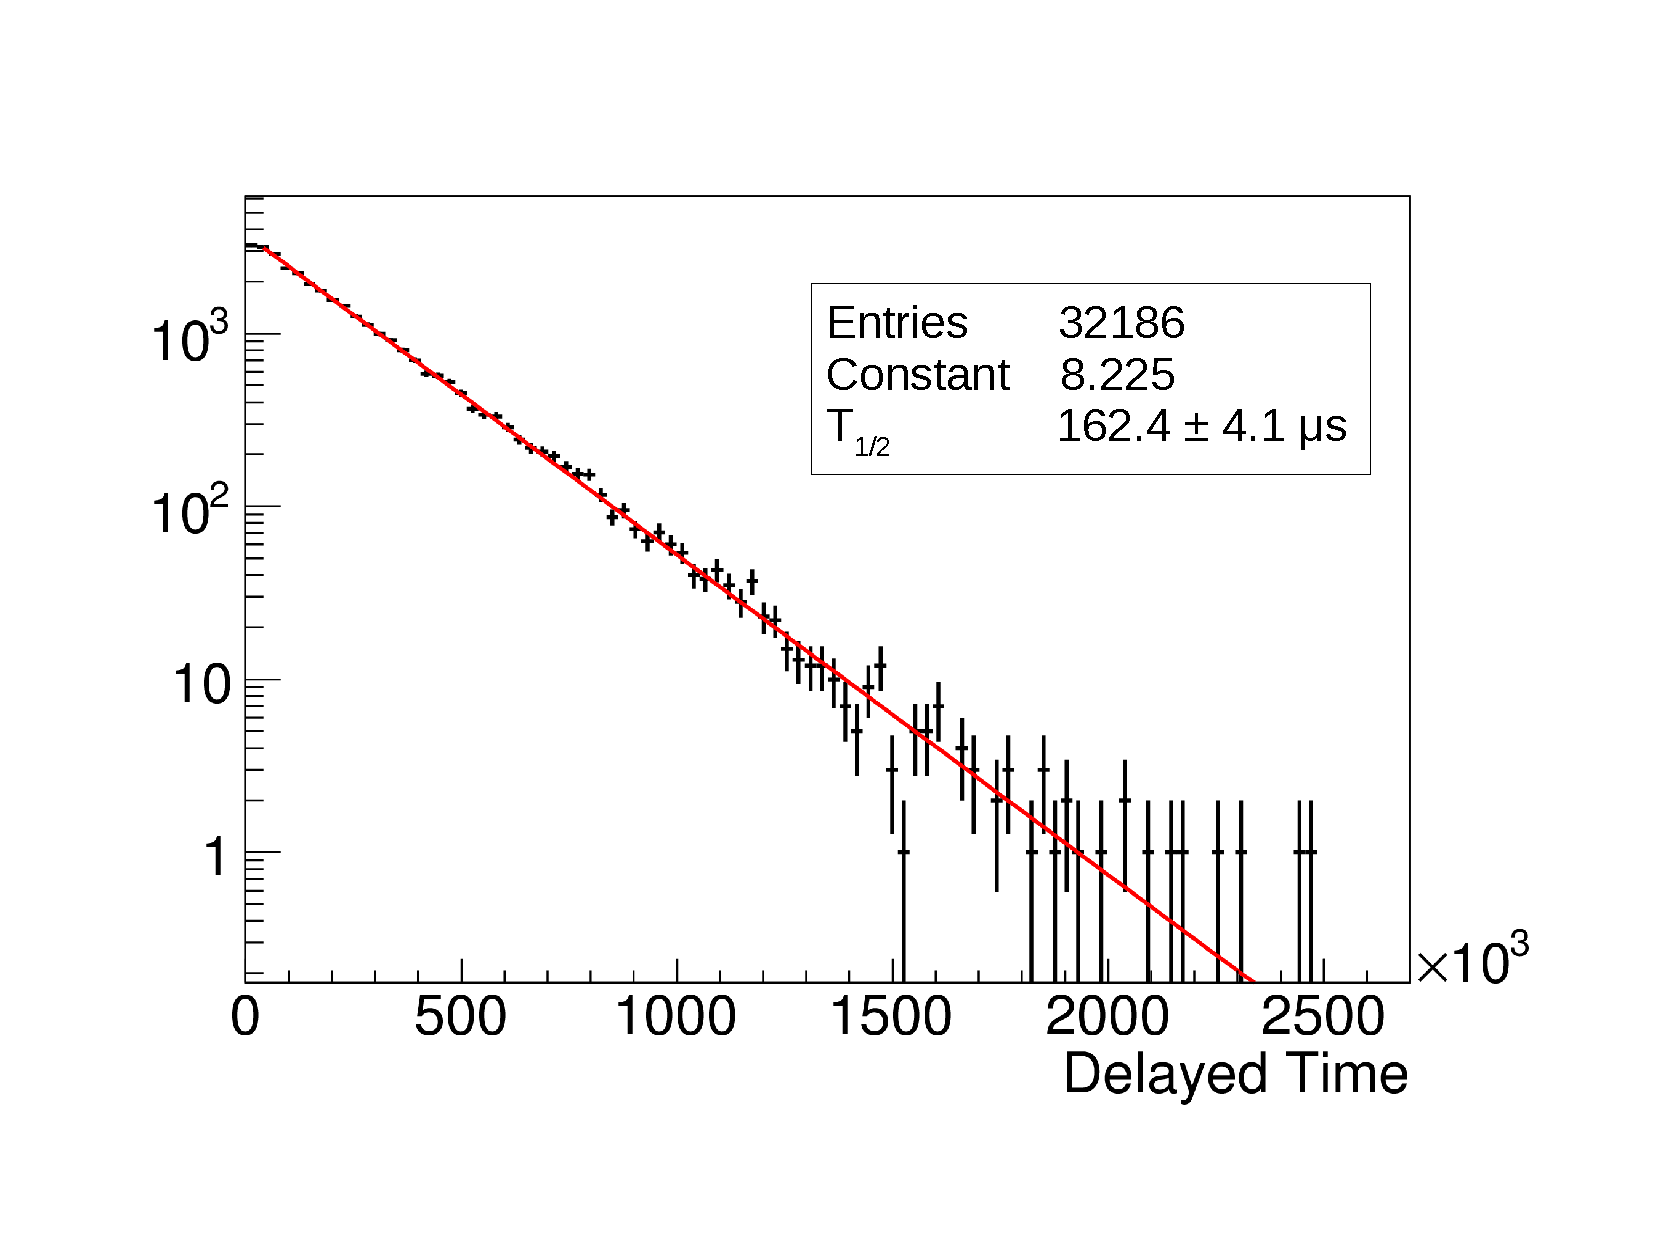
\includegraphics[scale=0.33]{pictures/Chap5/delayedtime.pdf}
\caption{Time between the alpha and the electron in the identified 1a1$\alpha$ channel with the source selection}
\label{delayedtimetopology}
\end{center}
\end{figure}


\bigskip


\noindent A last optimisation on the delay time is done. Indeed, if an electron triggers a very remote cell, the drift time can be greater than 10 $\mu$s thus categorizing the hit as delayed. This Geiger cell will then be mis-identified as an alpha particle by the Alpha Finder algorithm. An example of this kind of event, with a $"$fake$"$ alpha is shown in Figure~\ref{fakeAlpha}.


\begin{figure}[h!]
\begin{center}
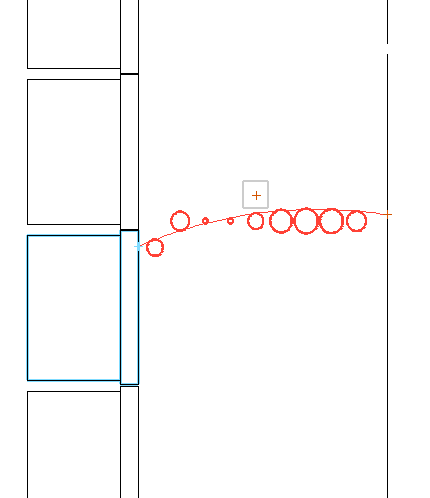
\includegraphics[scale=0.4]{pictures/Chap5/fakeAlpha.png}
\caption{Example of a fake alpha : a cell of the electron track (the square) is considered as delayed and identified by the Alpha Finder as an alpha particle.}
\label{fakeAlpha}
\end{center}
\end{figure}


\bigskip


\noindent The fake alphas lie tangent to the electron track thus the angle between the electron and the alpha $(\theta_{e-\alpha})$ is close to 0. Looking at the cos$( \theta_{e-\alpha})$ distribution, fake alphas will contribute at cos$(\theta_{e-\alpha}) \simeq$~1 as shown in Figure~\ref{angularDistribution}. The time distribution of the events which have cos $\theta_{e-\alpha}$ in~[0.95 - 1] is also plotted in Figure~\ref{angularDistribution}.


\begin{figure}[h!]
\begin{center}
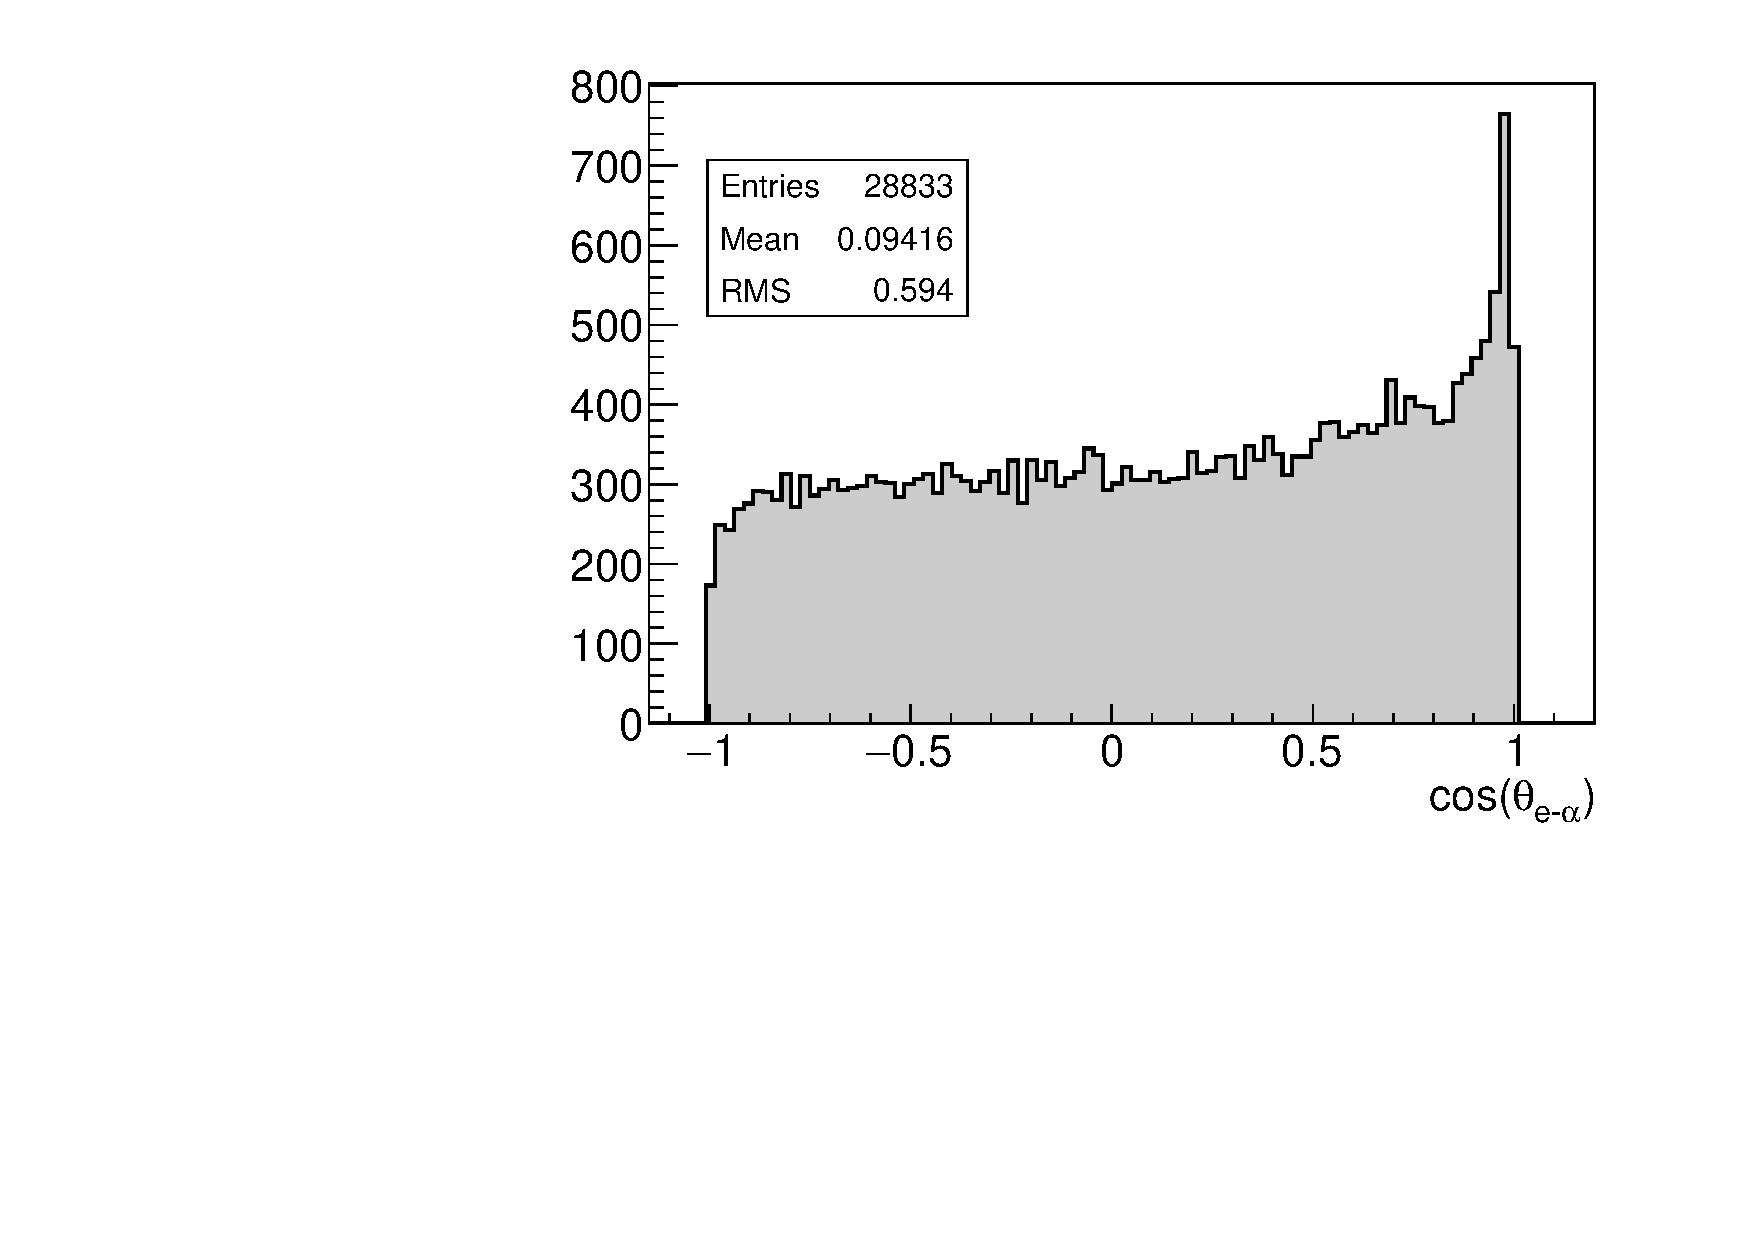
\includegraphics[scale=0.312]{pictures/Chap5/angle.pdf}
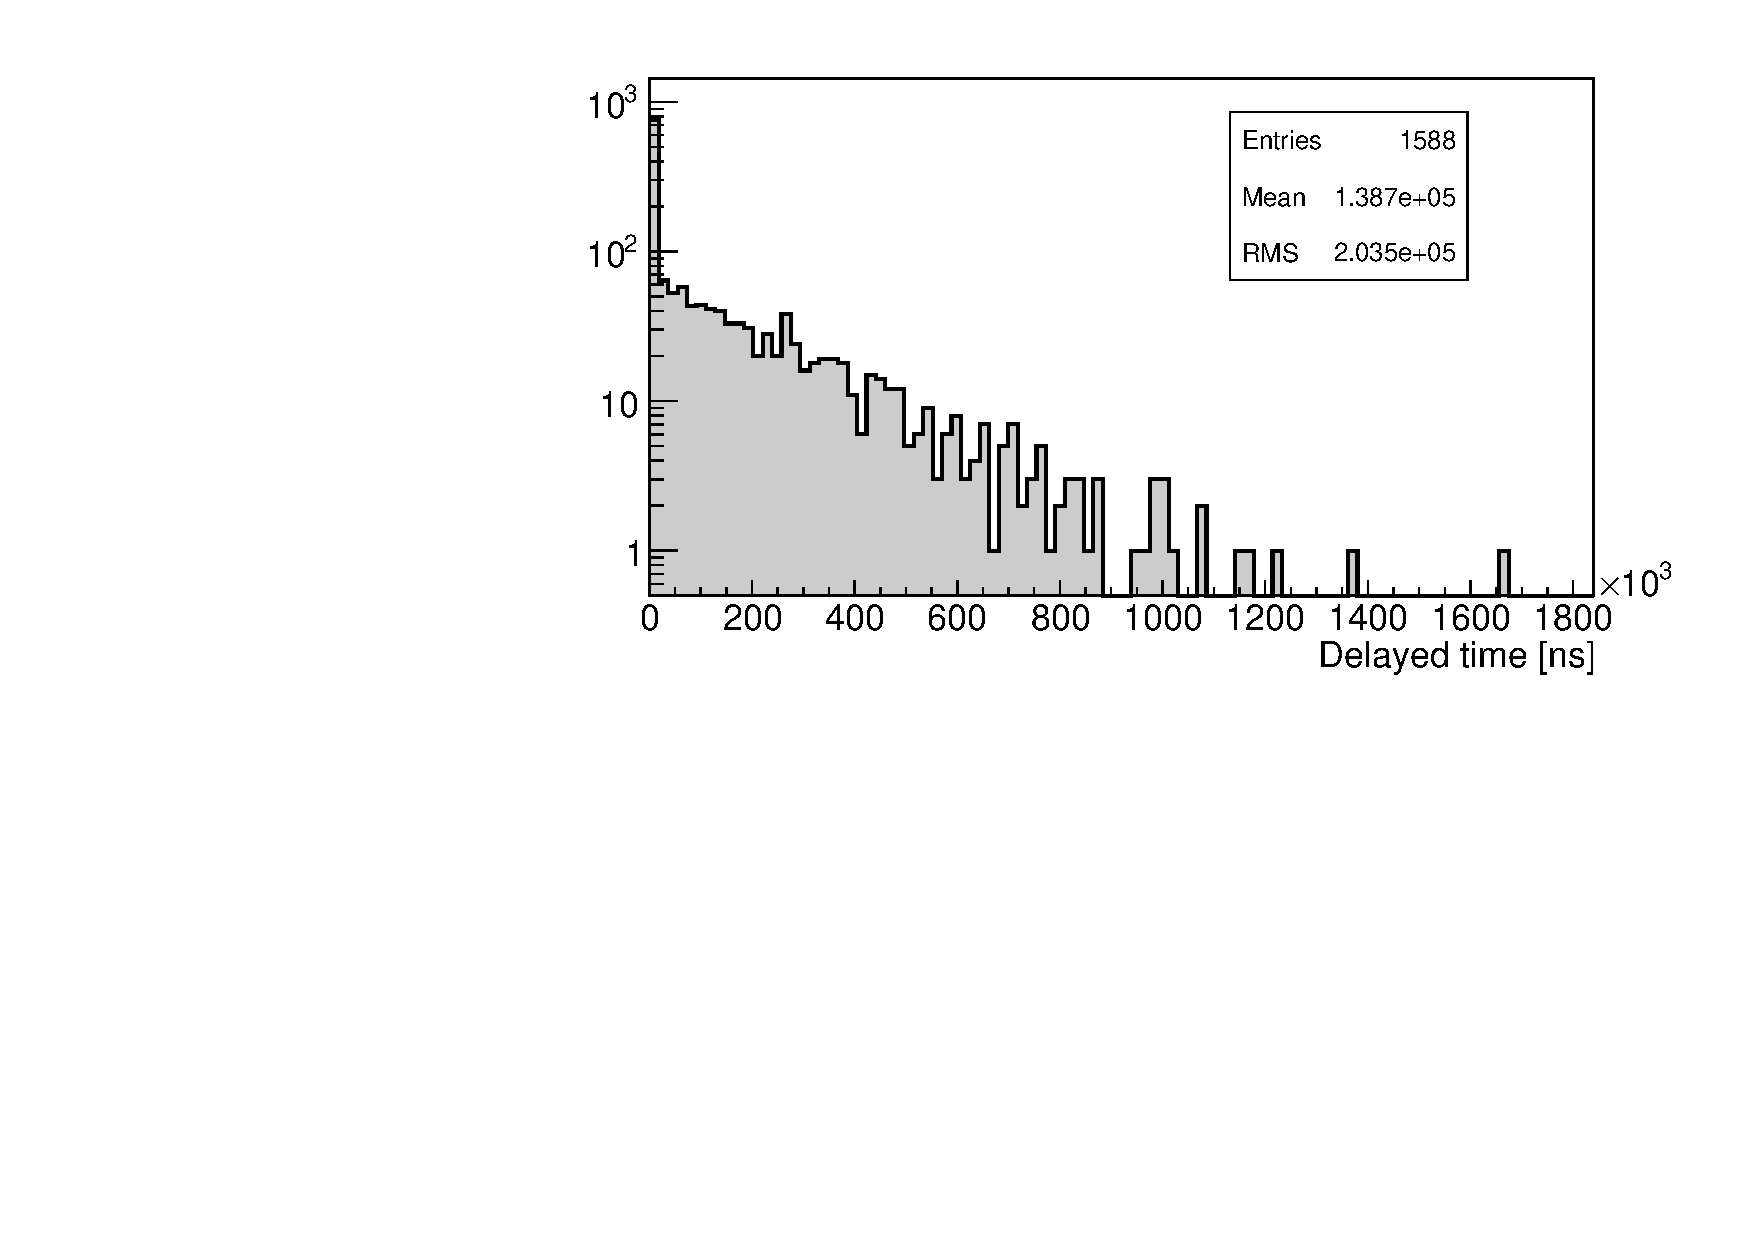
\includegraphics[scale=0.38]{pictures/Chap5/delayedTime.pdf}
%\includegraphics[scale=0.34]{/home/lenoblet-local/Documents/latex-papers/Alpha_Finder_note/pictures/angle_cut_optimisation.pdf}
\caption{On the left : The angular distribution of the 1e1$\alpha$ events with the fake alphas. The angle between the electron and the fake alpha is very close to zero, so an excess of events is expected near cos ($\theta_{e-\alpha}$) = 1. On the right : the time distribution for events with cos($\theta_{e-\alpha}$) in [0.95 - 1]. An excess of events corresponding to fake alphas is observed for very small $\Delta \text{t}$.} 
\label{angularDistribution}
\end{center}
\end{figure}

\bigskip

\noindent A peak is observed in the time distribution for the events having cos($\theta_{e-\alpha}$) $\simeq$ [0.95 - 1] so, the fake alphas have a different time distribution. The value of $\Delta \text{t}$ can thus be used as discriminating variable to remove the fake alphas. Knowing the true Monte Carlo information, we can check if the cell has been triggered by an alpha (true alpha event) or by an electron (fake alpha event) and study the two samples independently.


\begin{figure}[h!]
\begin{center}
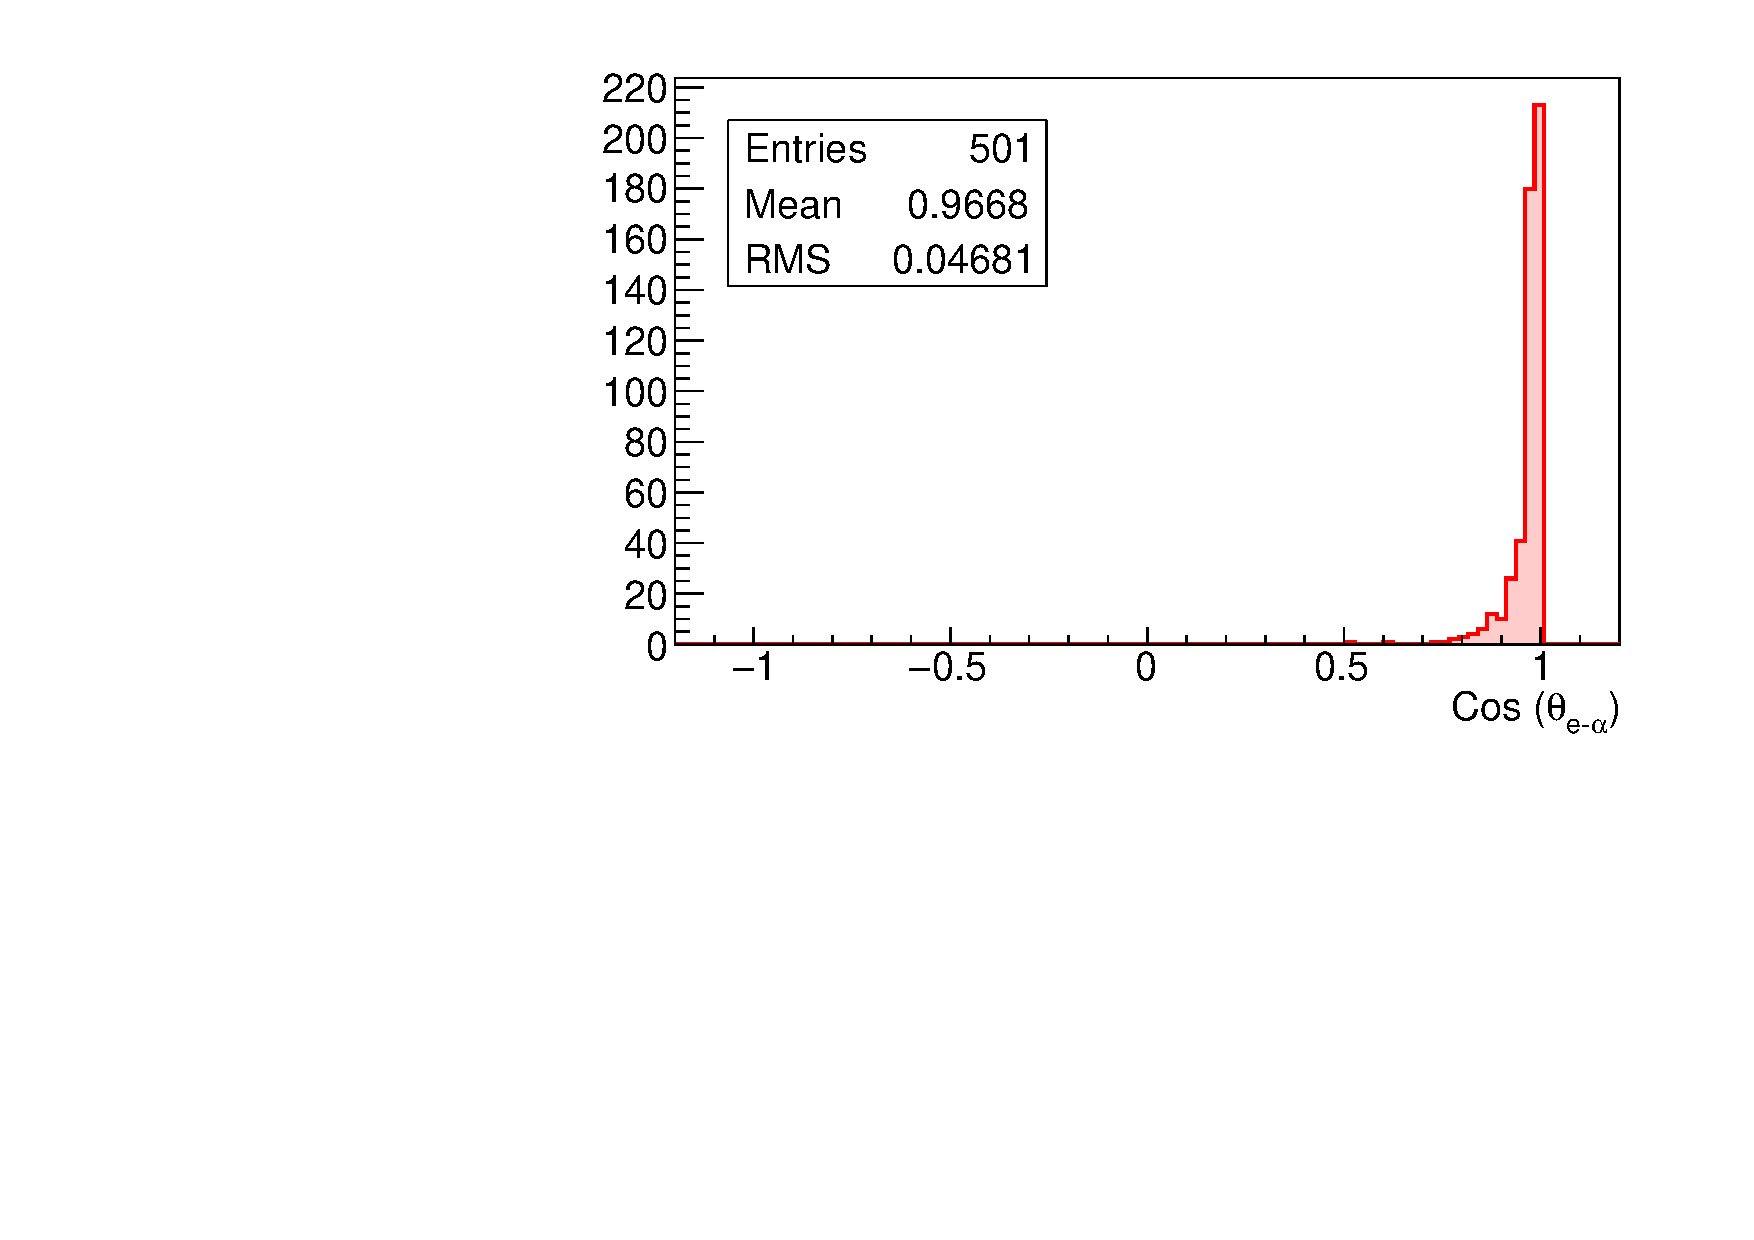
\includegraphics[scale=0.34]{pictures/Chap5/fake_alpha_angle_distribution.pdf}
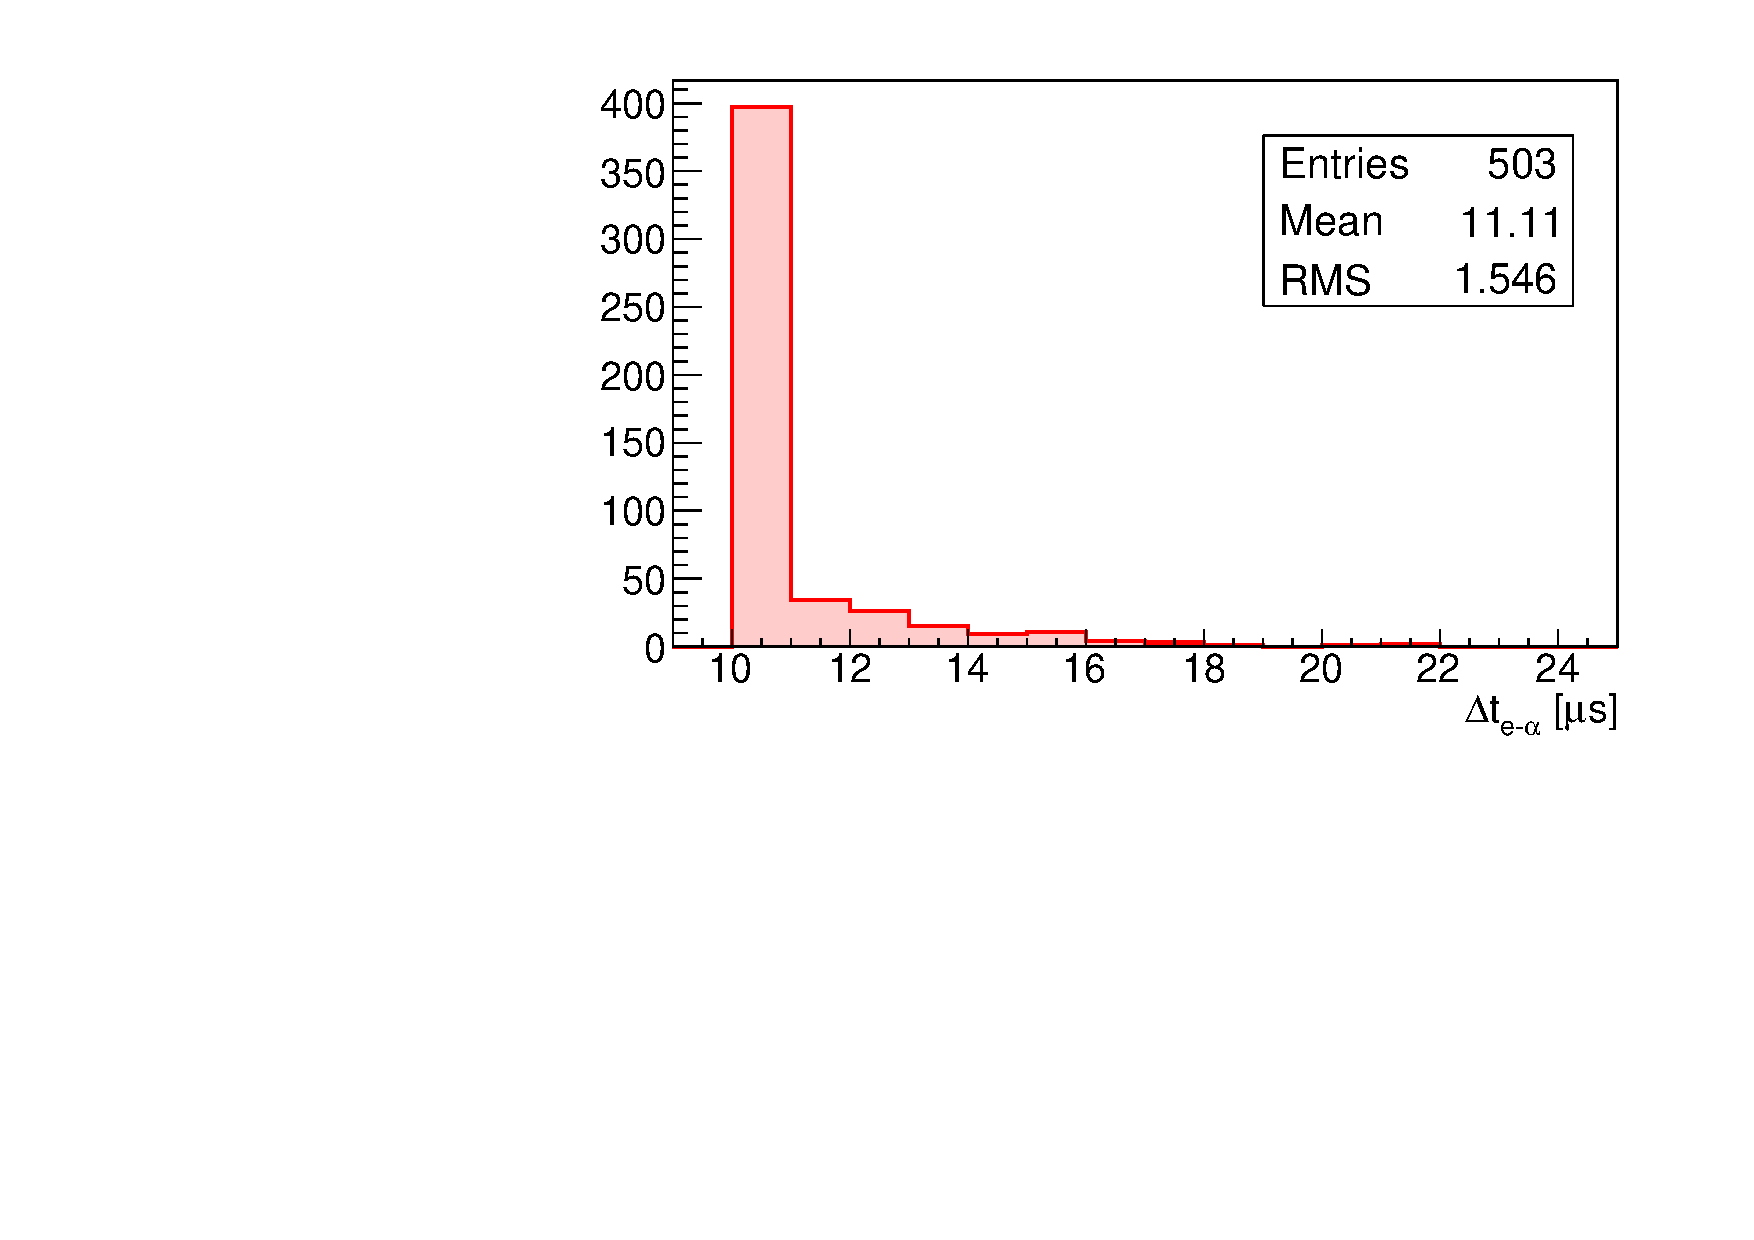
\includegraphics[scale=0.34]{pictures/Chap5/fake_alpha_time_distribution.pdf}
\caption{On the left : the angular distribution of the fake alpha. On the right : the time distribution of the fake alpha.}
\label{fakeAlphadistribution}
\end{center}
\end{figure}


\noindent The time and angular distribution of the fake alphas are plotted in Figure~\ref{fakeAlphadistribution}. The delay time of the fake alphas never exceeds 25~$\mu$s and, as expected, the angular distribution is peaked close to cos $\theta_{e-\alpha} =$~1. The same distributions are plotted in Figure~\ref{trueAlphadistribution} for the true alphas.


\begin{figure}[h!]
\begin{center}
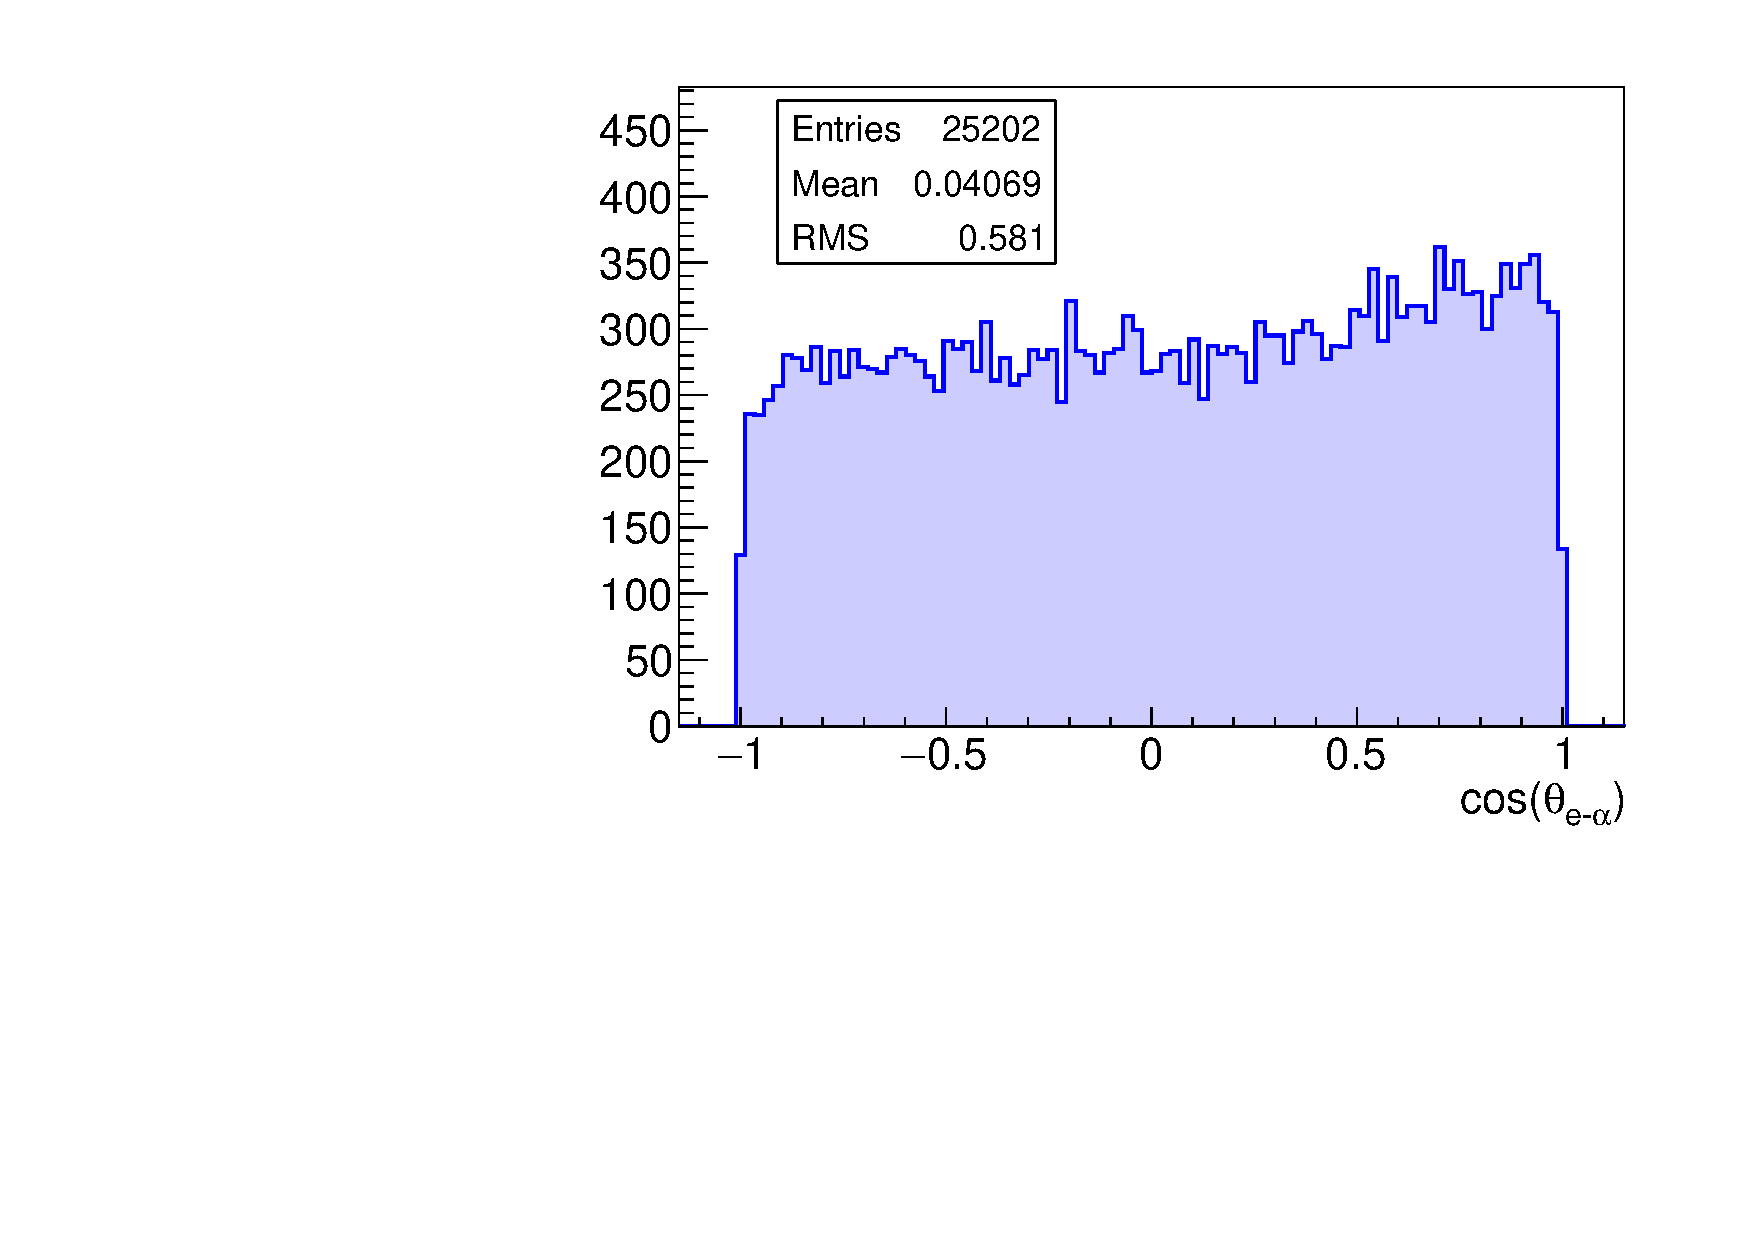
\includegraphics[scale=0.34]{pictures/Chap5/true_alpha_angle_distribution.pdf}
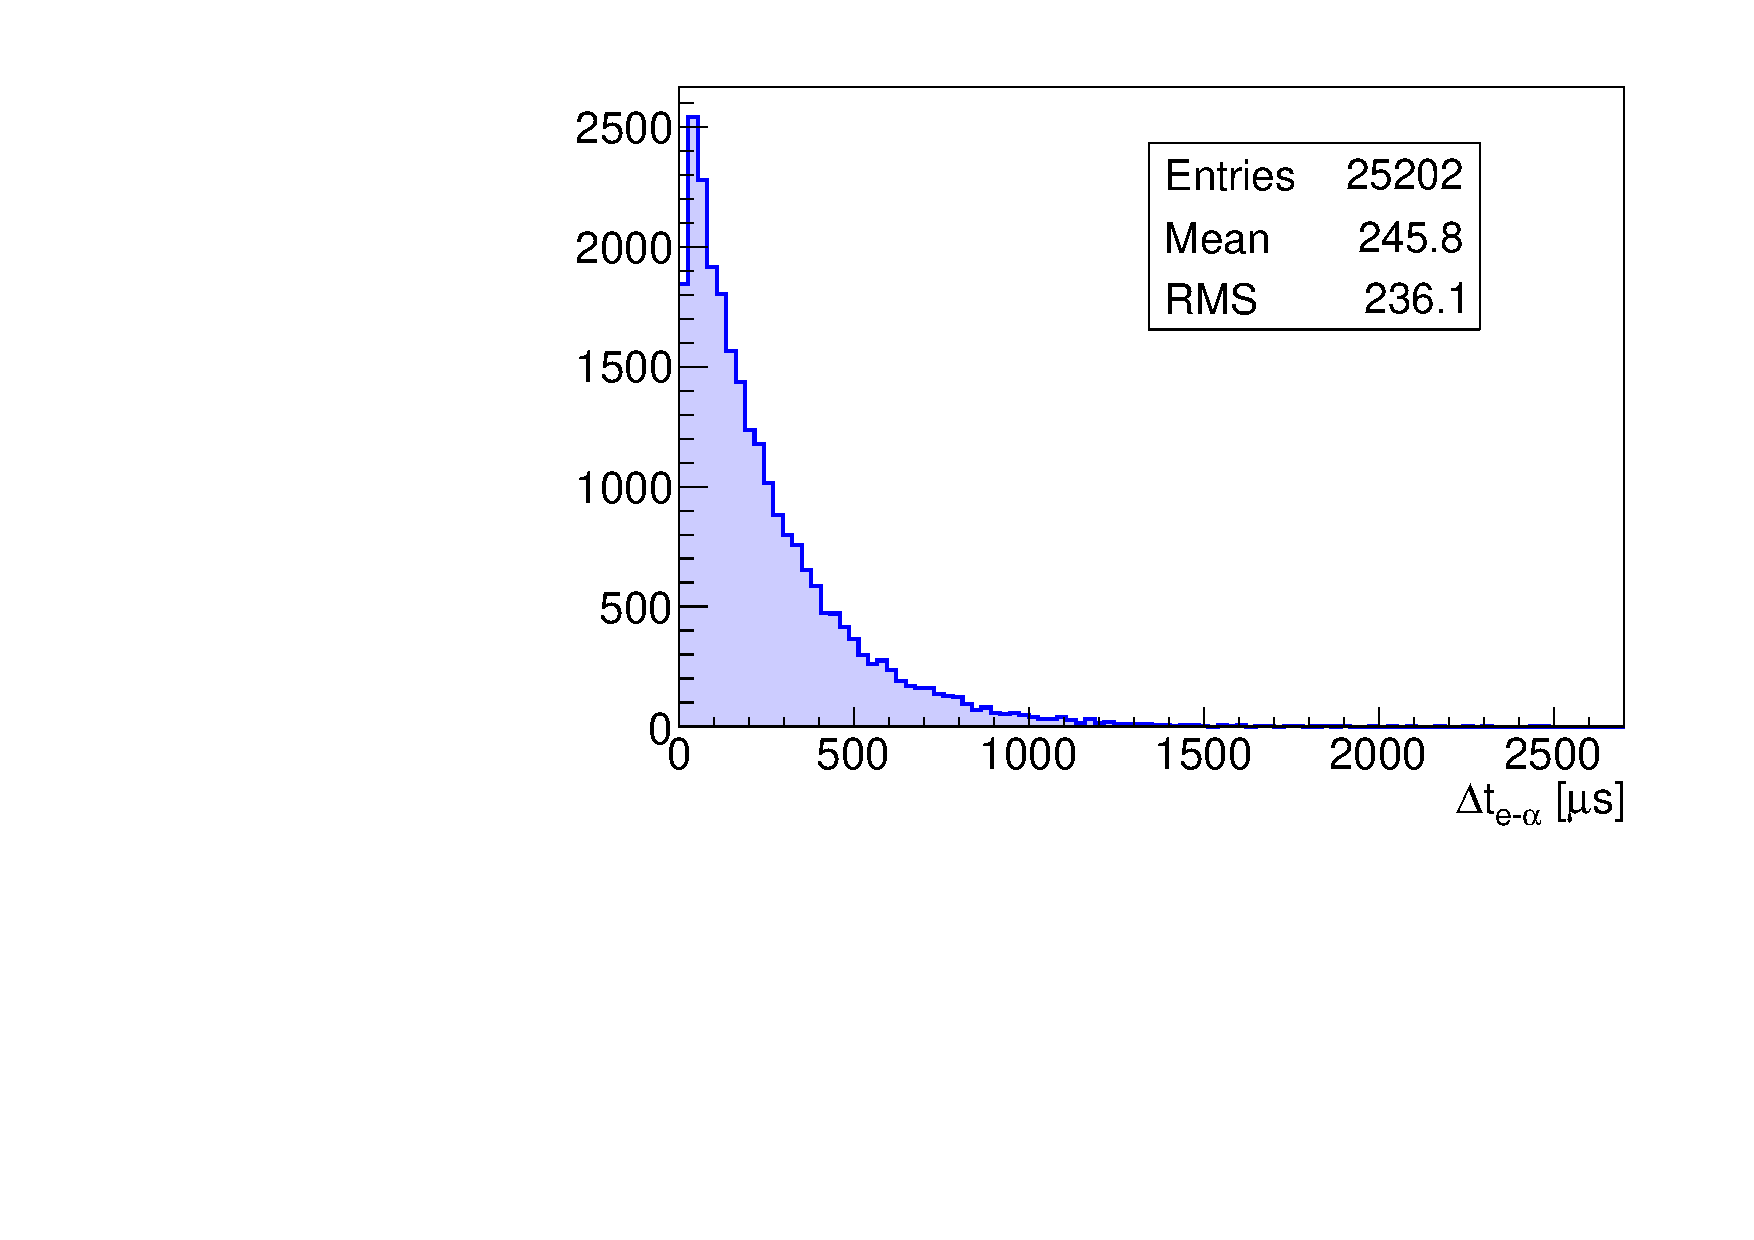
\includegraphics[scale=0.34]{pictures/Chap5/true_alpha_delayed_time.pdf}
\caption{On the left : the angular distribution of the true alphas. On the right : the time distribution of the true alphas (note the scale on the abcissa is much larger here).}
\label{trueAlphadistribution}
\end{center}
\end{figure}


\noindent In order to remove the maximum number of fake alphas but keep the maximum number of true alphas, the cut on $\Delta \text{t}$ has been optimized to maximize the product of the efficiency and purity ($\epsilon \times \text{p}$). The efficiency of the cut, is defined by the fraction of fake alphas removed by the cut at~$\Delta \text{t}$~:


\begin{equation}
\epsilon = \frac{ \displaystyle{\int_0^{\Delta \text{t}}} \text{f(t)} \text{dt} } { \displaystyle{\int_\text{0}^{+\infty}} \text{f(t)} \text{dt}} 
\end{equation}


\noindent where f(t) is the time distribution of the fake alphas. In the same way, the purity is defined as the fraction of the true alphas kept after the cut $\Delta t$~:

\begin{equation}
\text{p} = \frac{ \displaystyle{\int_{\Delta \text{t}}^{+\infty}} \text{g(t)} \text{dt} } { \displaystyle{\int_\text{0}^{+\infty}} \text{g(t)} \text{dt}} 
\end{equation}

\noindent where g(t) is the time distribution of the true alphas. The efficiency of the cut (in~red) and the purity (in~blue) as a function of cut value $\Delta \text{t}$ is shown in Figure~\ref{efficiency_ratio}. The product of the efficiency and the purity versus delay time is also plotted in Figure~\ref{efficiency_ratio}.


\begin{figure}[h!]
\begin{center}
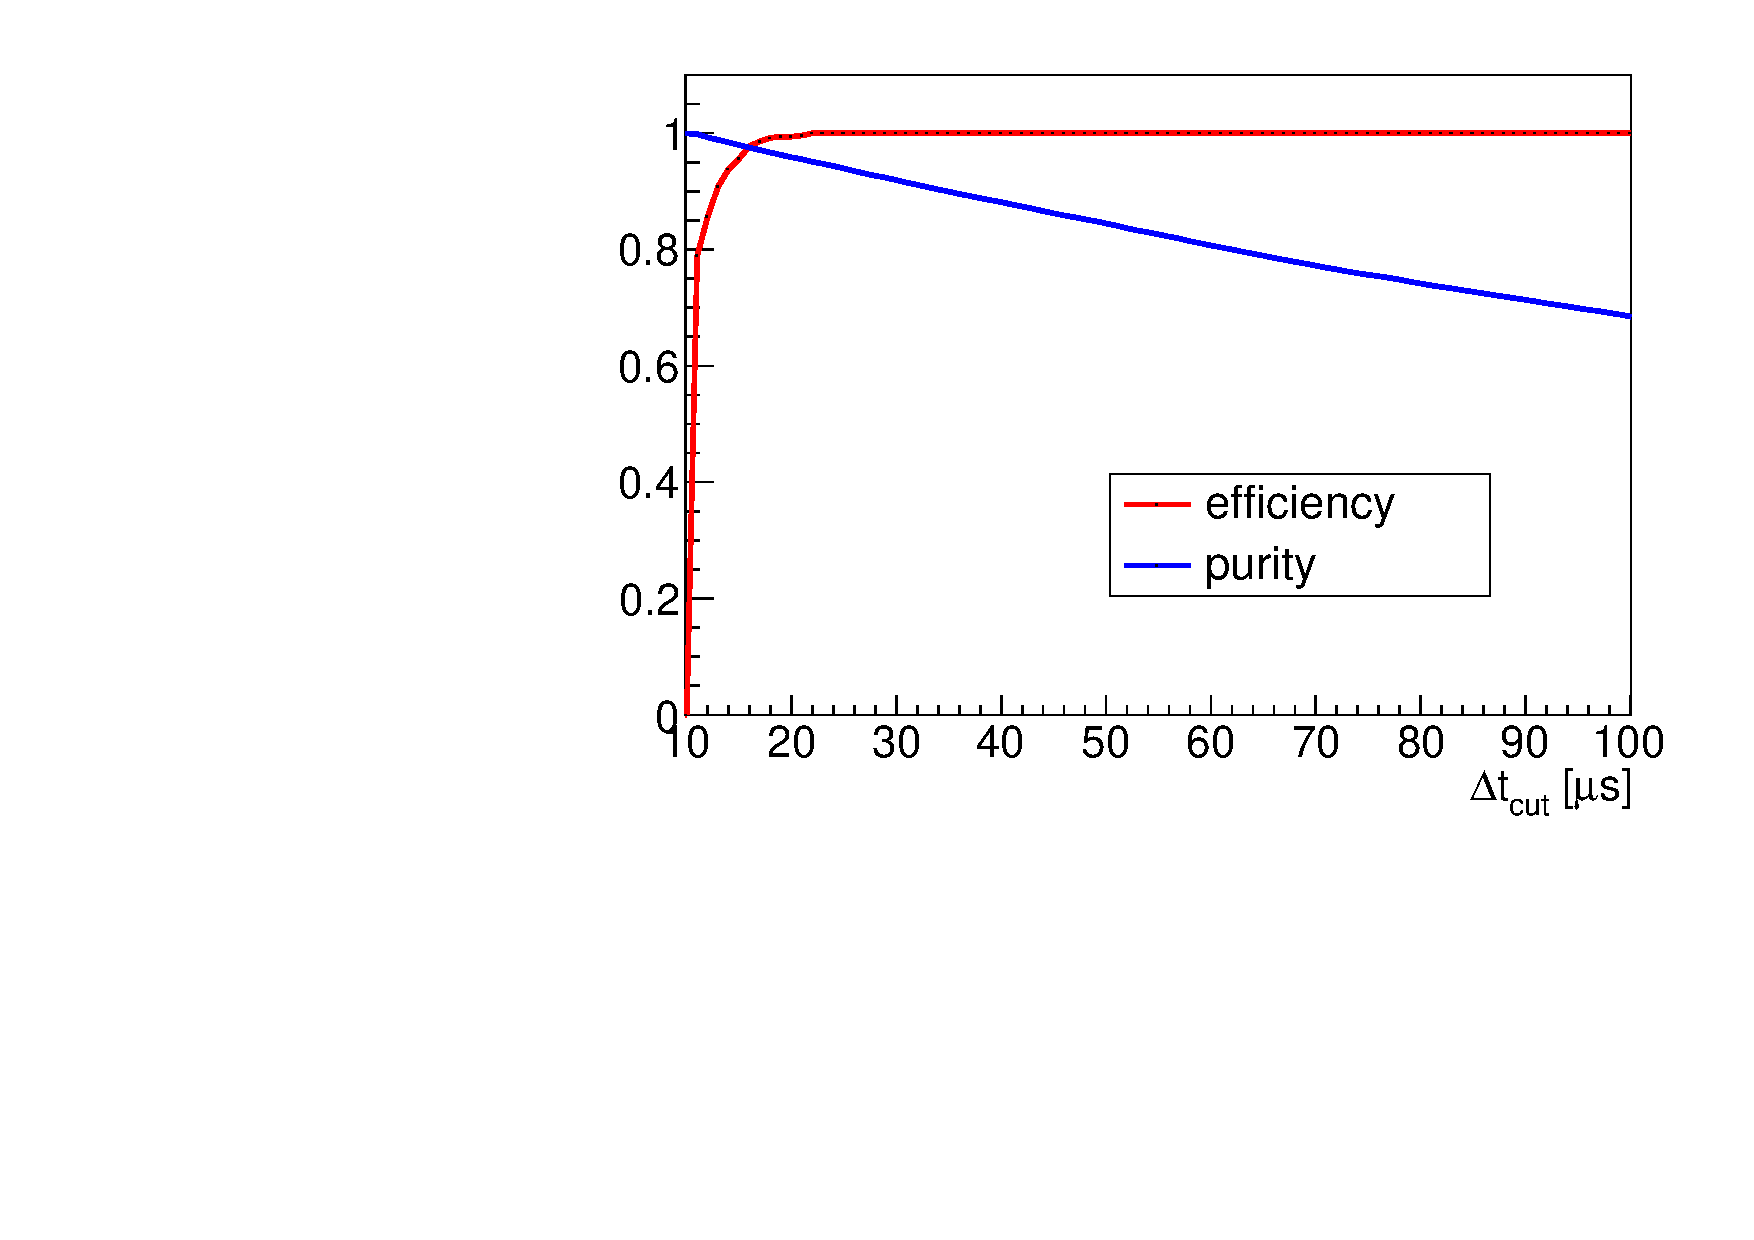
\includegraphics[scale=0.4]{pictures/Chap5/efficiency_purity.pdf}
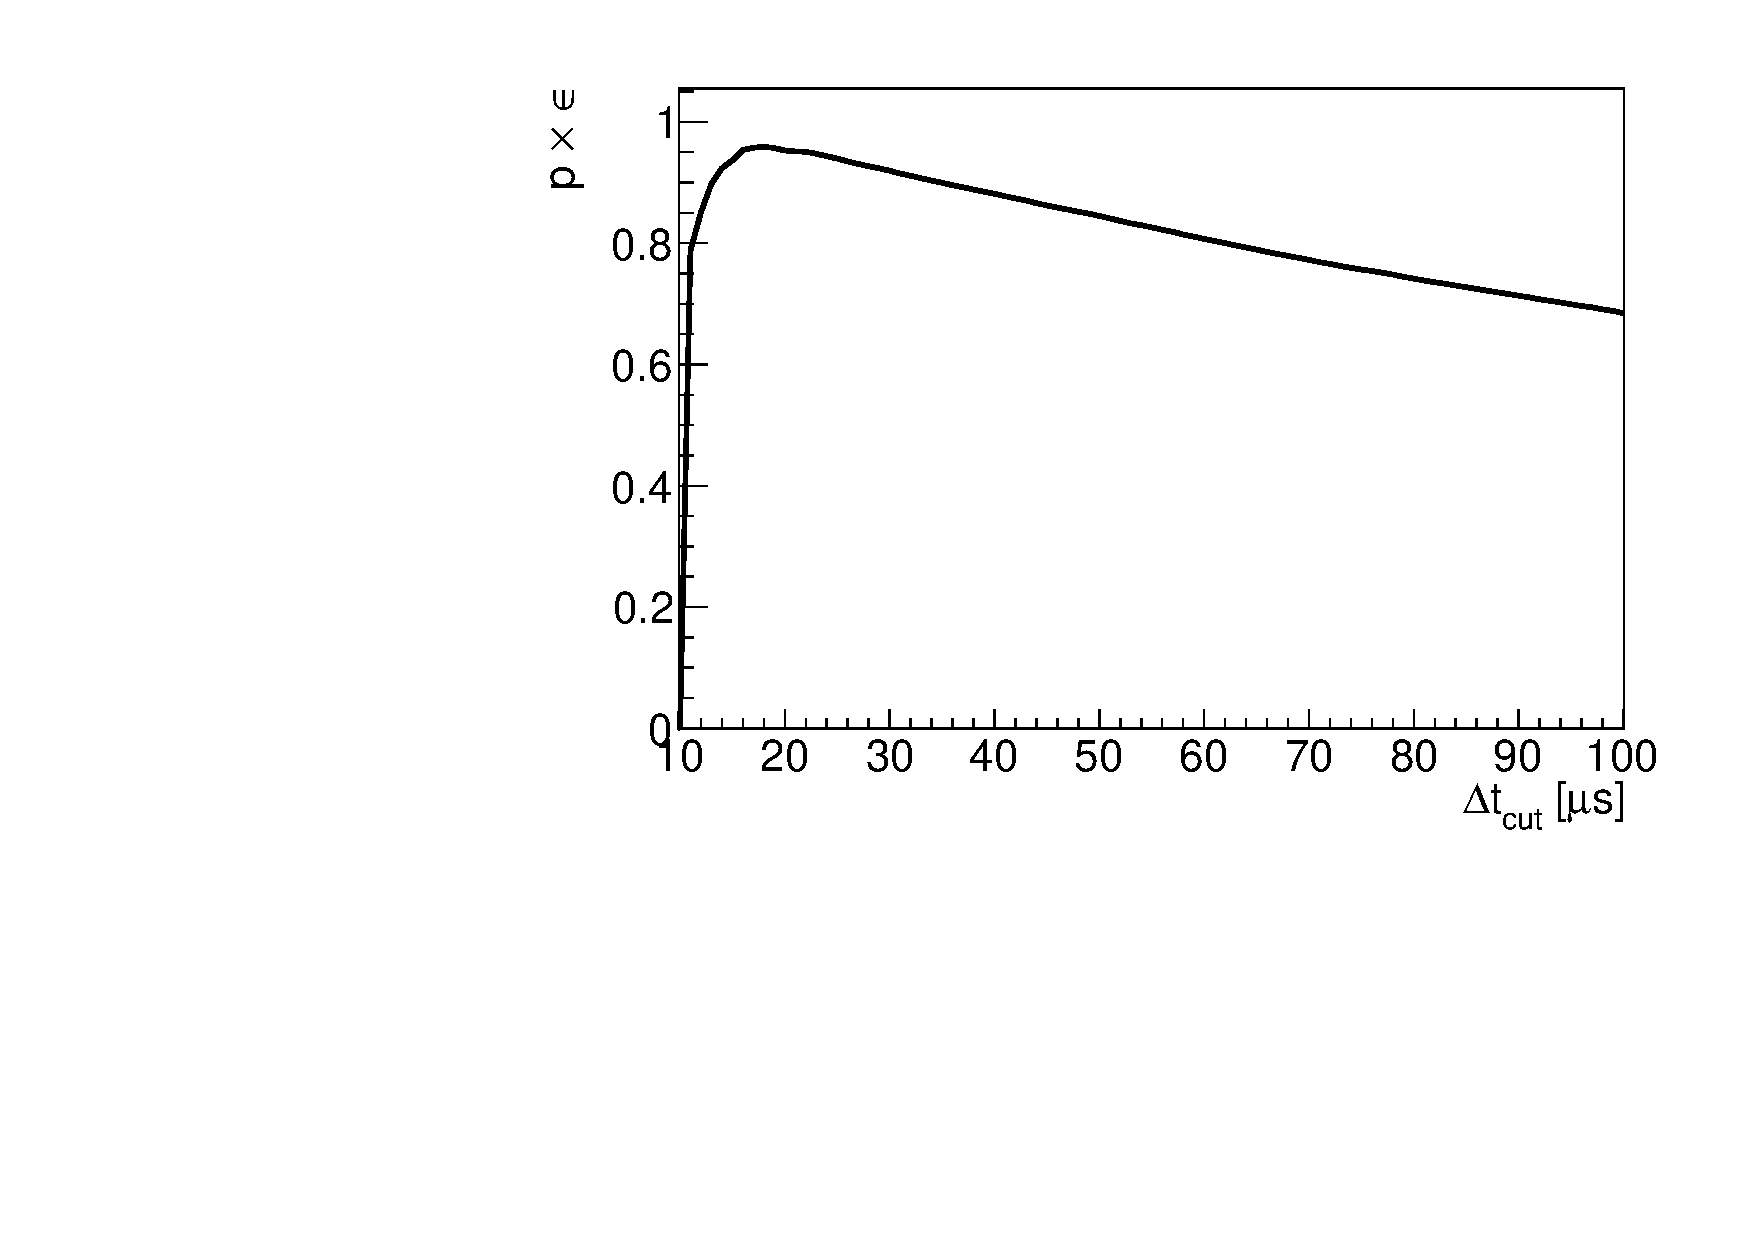
\includegraphics[scale=0.4]{pictures/Chap5/pe.pdf}
\caption{Left : the efficiency of the cut for the true alphas in blue and the fake alphas in red. Right : the product of the two efficiencies. This product has a maximum for a cut at $\Delta \text{t}_{e-\alpha}$ = 17.0 $\mu$s.}
\label{efficiency_ratio}
\end{center}
\end{figure}

\bigskip

\noindent The product is maximized for a cut at $\Delta \text{t}_{e-\alpha} =$ 17.0~$\mu$s. By selecting only events with $\Delta \text{t}_{e-\alpha} >$ 17.0 $\mu$s, 98.6~$\%$ of the fake alphas are removed and only 2.9~$\%$ of true alphas are lost.

\bigskip

\noindent The number of reconstructed 1e1$\alpha$ events depending on the vertex is given in the Table \ref{efficiency_different_parts_foil_source}. So, $\sim$ 10~\% of the 1e1$\alpha$ events generated on the surface of the foil are reconstructed. The efficiency of reconstruction of the 1e1$\alpha$ events coming from the bulk is $\sim$ 3~\%. With the source selection, $\sim$ 1.5\% of the 1e1$\alpha$ events coming from the tracker are reconstructed. These events are the events generated on the first layer of tracker wires close to the source foil. By default, the vertex is extrapolated to the source if the first layer of wire is hit.


\begin{table}[h!]
\begin{center}
\begin{tabular}{c|c|c|c}
           & bulk   & surface & tracker \\
\hline
$\epsilon_{\text{1e1}\alpha}$ [\%] & 2.94 & 10.07  & 1.59 \\
\hline
\end{tabular}
\end{center}
\caption{Summary of the efficiency, in different parts of the detector, computed with the Monte-Carlo.}
\label{efficiency_different_parts_foil_source}
\end{table}


\FloatBarrier


\subsection{1e1$\alpha$ events from the tracker}


\noindent A picture representing the 1e1$\alpha$ selection of the event coming from the tracker is shown in Figure~\ref{cartoon_tracker_selection}. Only the events having their vertex in the green region (in the tracker except the first layer of wire close to the source) are selected.

 
\begin{figure}[h!]
\begin{center}
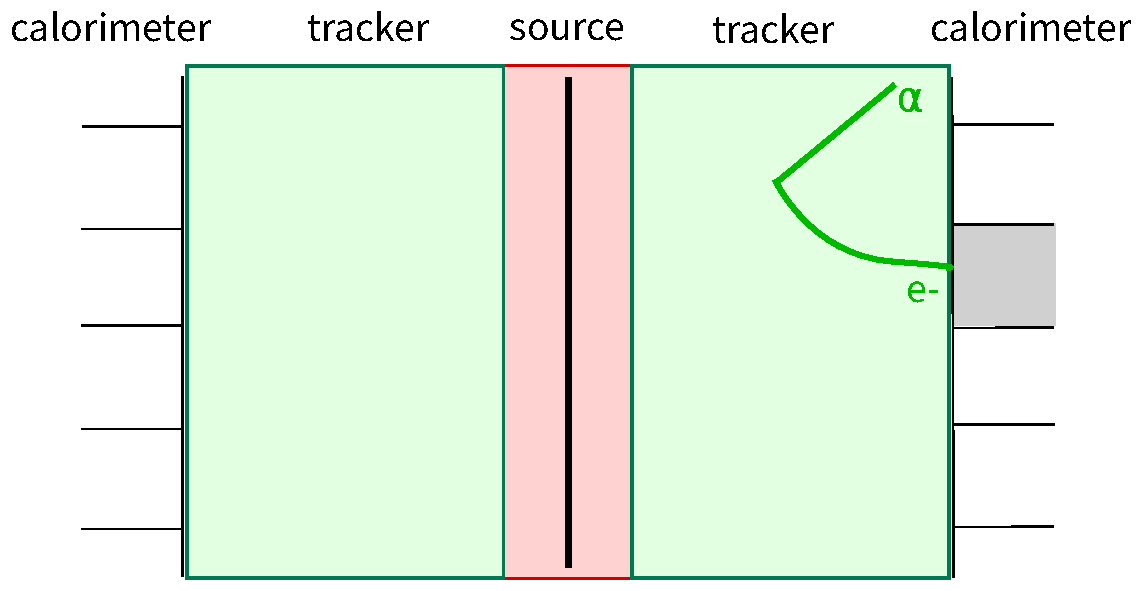
\includegraphics[scale=0.6]{pictures/Chap5/cartoon_tracker_selection.pdf}
\caption{Tracker selection diagram of the tracker selection. The green part represents the region where the events are selected.}
\label{cartoon_tracker_selection}
\end{center}
\end{figure}


\noindent In this selection, an electron is defined as a prompt particle hitting a calorimeter. To increase the statistics, an electron can also hit the main wall, the $\gamma$-veto wall, or the x-wall. Generated in the tracker, some electrons are expected to be simulated very close to a calorimeter block and will not have a long track. In some cases, electron tracks can be only 2-3 Geiger hits even appearing on a straght line. So, the same study about the charge confusion is realized.


\bigskip


\noindent The electron length and the charge confusion are plotted in Figure \ref{charge_confusion_tracker_plots}. The charge confusion is high for the short length and reaches 80~\%. The charge confusion decreases with the length of the track and reaches a stable value of ~20~\% for tracks longer than 50~cm.


\begin{figure}[h!]
\begin{center}
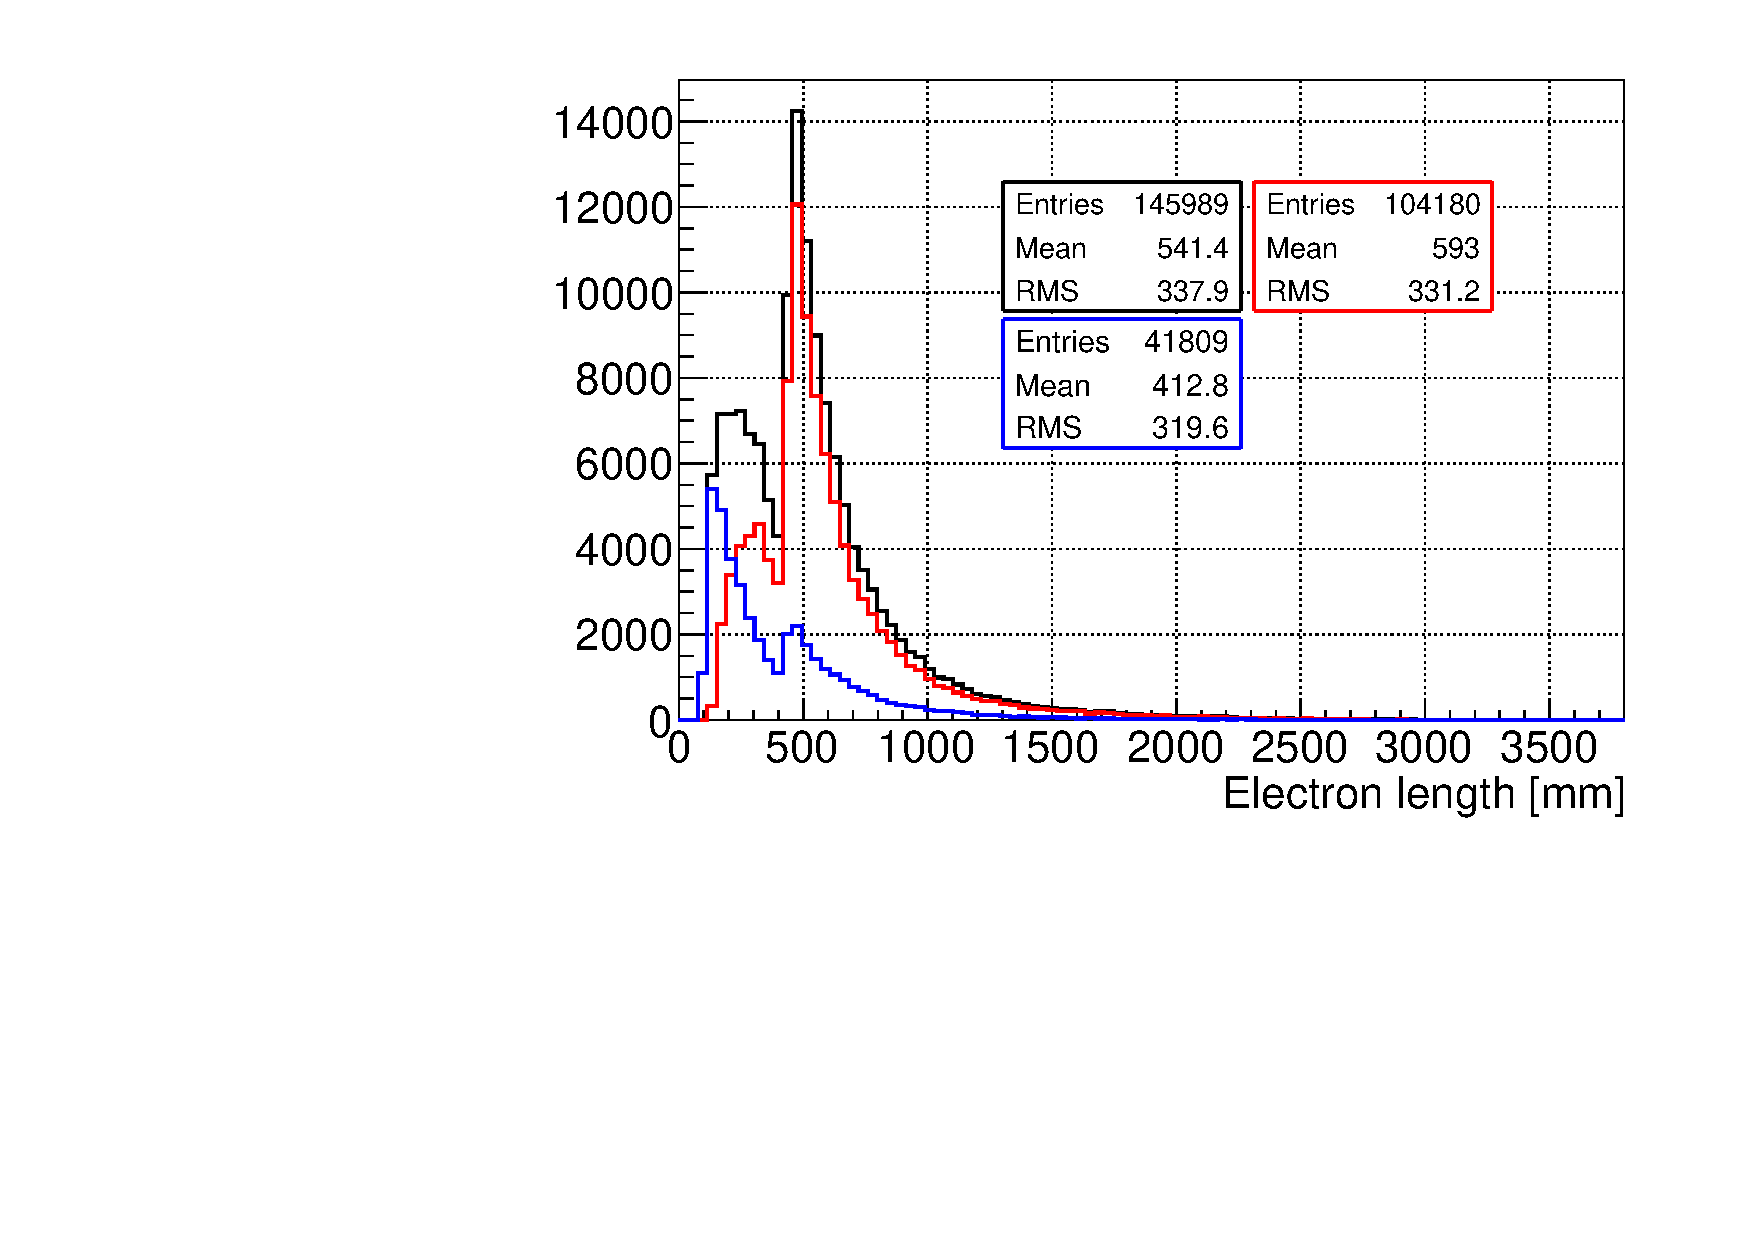
\includegraphics[scale=0.35]{pictures/Chap5/length_tracker_charge_confusion_2.pdf}
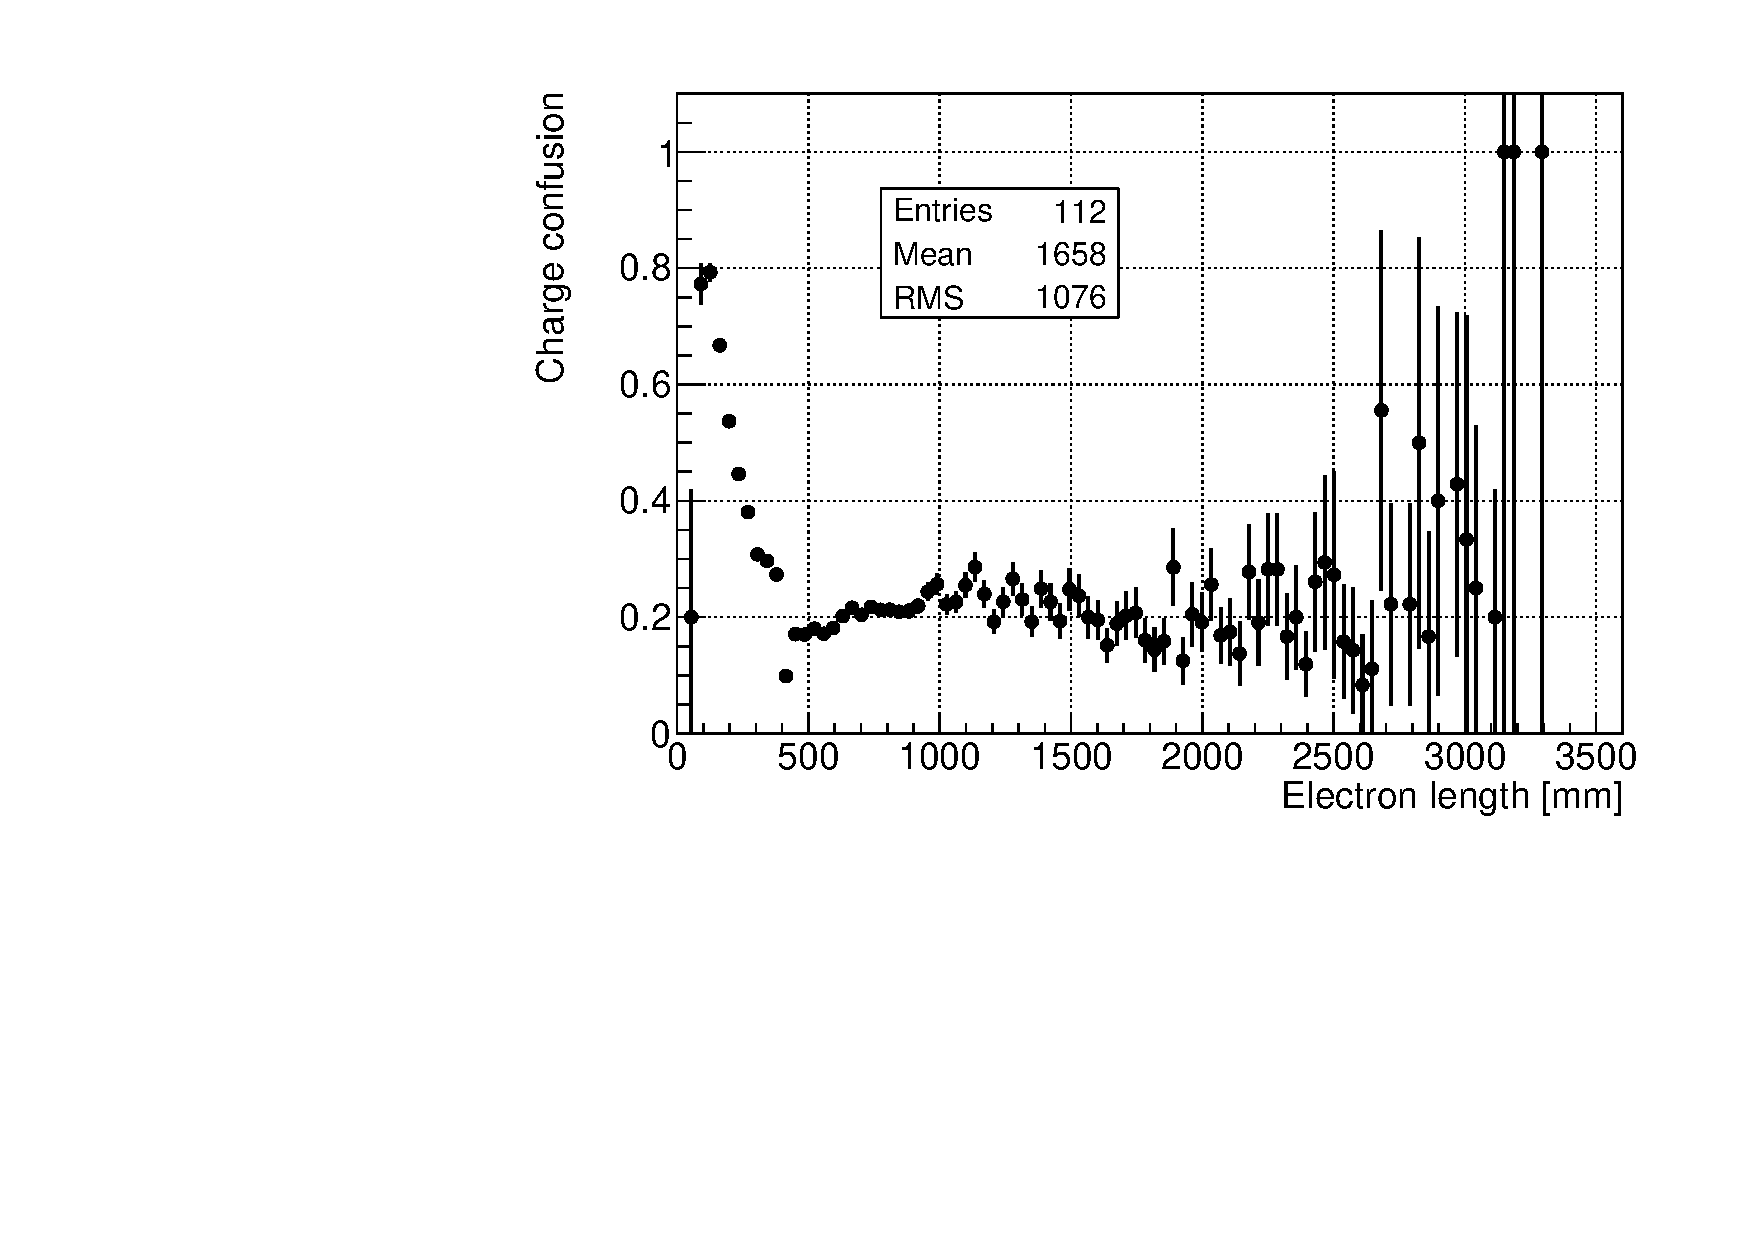
\includegraphics[scale=0.35]{pictures/Chap5/charge_confusion_length_tracker.pdf}
\caption{On the left : length of the electron vs the charge. The black curve represents all the reconstructed electrons hitting a calorimeter. In red, the electrons hitting a calorimeter reconstructed with a negative charge. In blue, the electrons reconstructed with a positive or undefined charge. On the right : the charge confusion vs the length of the electron track.}
\label{charge_confusion_tracker_plots}
\end{center}
\end{figure}


\bigskip 


\noindent If a cut is introduced to select the electrons reconstructed with a negative charge, $\sim$27~\% of the true electrons are lost. So, in order to avoid losing too many events, no cut on the charge is introduced. The cut flow of the electrons coming from the tracker is summarized in Table~\ref{Cutflowelectrontracker}. 

\begin{table}[h!]
\begin{center}
\begin{tabular}{l|c|c}
 & N & $\epsilon$ \\
\toprule
$\#$ of simulated electrons & 308 000 & \\
\hline
$\#$ of reconstructed electrons & 385 176 & 125.0 $\pm$ 0.2 \% \\
$\#$ coming from the tracker    & 385 176 & 125.0 $\pm$ 0.2 \%\\
$\#$ hiting the main wall       & 144 187 & 46.8  $\pm$ 0.2 \%\\
$\#$ having a negative charge   & 78 940  & 25.6  $\pm$ 0.2 \%\\
\bottomrule
\end{tabular}
\end{center}
\caption{Cut flow of the electrons coming from the tracker. The efficiencies are computed by dividing by the number of simulated electrons.}
\label{Cutflowelectrontracker}
\end{table}


\bigskip


\noindent By releasing the cut on the charge and allowing an electron to hit the x-wall or the $\gamma$ veto, the selection of the electron in the tracker is $\sim$ 25~\%. The cut flow of the electrons coming from the bulk and the surface of the foil are summarized in Table~\ref{Cutflowelectrontrackerbulk} and Table~\ref{Cutflowelectrontrackersurface}.


\begin{table}[h!]
\begin{center}
\begin{tabular}{l|c|c}
 & N & $\epsilon$ \\
\toprule
$\#$ of simulated electrons & 308 000 & \\
\hline
$\#$ of reconstructed electrons & 320 379 & 104.0 $\pm $0.2 \% \\
$\#$ coming from the tracker    & 320 379 & 104.0 $\pm$ 0.2 \%\\
$\#$ hiting the main wall       & 161 308 & 53.8 $\pm$ 0.2 \%\\
$\#$ having a negative charge   & 17 088  & 5.4 $\pm$ 0.2 \%\\
\bottomrule
\end{tabular}
\end{center}
\caption{Cut flow of the electrons coming from the bulk. The efficiencies are computed by dividing by the number of simulated electrons.}
\label{Cutflowelectrontrackerbulk}
\end{table}

\begin{table}[h!]
\begin{center}
\begin{tabular}{l|c|c}
 & N & $\epsilon$ \\
\toprule
$\#$ of simulated electrons & 308 000 & \\
\hline
$\#$ of reconstructed electrons & 362 157 & 117.6 $\pm$ 0.2 \% \\
$\#$ coming from the tracker    & 362 157 & 117.6 $\pm$ 0.2 \%\\
$\#$ hiting the main wall       & 159 893 & 51.9 $\pm$ 0.2 \%\\
$\#$ having a negative charge   & 21 567  & 7.0 $\pm$ 0.2 \%\\
\bottomrule
\end{tabular}
\end{center}
\caption{Cut flow of the electrons coming from the surface. The efficiencies are computed by dividing by the number of simulated electrons.}
\label{Cutflowelectrontrackersurface}
\end{table}


\bigskip

\noindent As expected, the selection efficiency of the electrons coming from the foil is low, $\sim$~6\% and $\sim$~7\%. This corresponds to electrons coming from the source foil that did not trigger the first layer of wires of the tracker. The vertex of these events is reconstructed in the tracker even if they come from the source foil.  


\bigskip


\noindent An alpha is defined as a particle delayed in time hitting no calorimeter and not coming from the source. The cut flow of the alpha of the tracker is summarized in Table~\ref{Cutflowalphatrackertracker}, in Table~\ref{Cutflowalphatrackerbulk} (bulk) and Table~\ref{Cutflowalphatrackersurface} (surface).


\begin{table}[h!]
\begin{center}
\begin{tabular}{l|c|c}
 & N & $\epsilon$ \\
\toprule
$\#$ of simulated alphas & 300 000 & \\
\hline
$\#$ of reconstructed alpha & 131 596 & 43.9 $\pm$ 0.2 \%\\
$\#$ being delayed          & 131 596 & 43.9 $\pm$ 0.2 \%\\
$\#$ coming from the tracker& 98 880  & 33.0 $\pm$ 0.2 \%\\
$\#$ hitting no calorimeter & 98 859  & 33.0 $\pm$ 0.2 \%\\
\bottomrule
\end{tabular}
\end{center}
\caption{Cut flow of the alpha coming from the tracker. The efficiencies are computed by dividing by the number of simulated alphas.}
\label{Cutflowalphatrackertracker}
\end{table}


\begin{table}[h!]
\begin{center}
\begin{tabular}{l|c|c}
 & N & $\epsilon$ \\
\toprule
$\#$ of simulated alphas & 300 000 & \\
\hline
$\#$ of reconstructed alpha & 33 876 & 11.3 $\pm$ 0.2 \%\\
$\#$ being delayed          & 33 876 & 11.3 $\pm$ 0.2 \%\\
$\#$ coming from the tracker& 9 570  & 3.19 $\pm$ 0.2 \%\\
$\#$ hitting no calorimeter & 9 565  & 3.19 $\pm$ 0.2 \%\\
\bottomrule
\end{tabular}
\end{center}
\caption{Cut flow of the alpha coming from the tracker. The efficiencies are computed by dividing by the number of simulated alphas.}
\label{Cutflowalphatrackerbulk}
\end{table}


\begin{table}[h!]
\begin{center}
\begin{tabular}{l|c|c}
 & N & $\epsilon$ \\
\toprule
$\#$ of simulated alphas & 300 000 & \\
\hline
$\#$ of reconstructed alpha & 104 288 & 34.8 $\pm $0.2 \%\\
$\#$ being delayed          & 104 288 & 34.8 $\pm $0.2 \%\\
$\#$ coming from the tracker& 16 972  & 5.66 $\pm $0.2 \%\\
$\#$ hitting no calorimeter & 16 972  & 5.66 $\pm $0.2 \%\\
\bottomrule
\end{tabular}
\end{center}
\caption{Cut flow of the alpha coming from the surface. Cut flow of the alpha coming from the tracker. The efficiencies are computed by dividing by the number of simulated alphas.}
\label{Cutflowalphatrackersurface}
\end{table}


\bigskip


\noindent The 1e1$\alpha$ topology is built by associating, an electron and a delayed alpha. The alpha length of the different contributions are plotted in Figure~\ref{alpha_length_tracker_selection}. The delayed time between the electron and the alpha is shown in Figure~\ref{delta_t_tracker_selection}. The optimisation introduced in the previous section on the $\Delta$t~>~17~$\mu$s is also applied because it does not depend on the vertex position. 


\begin{figure}[h!]
\begin{center}
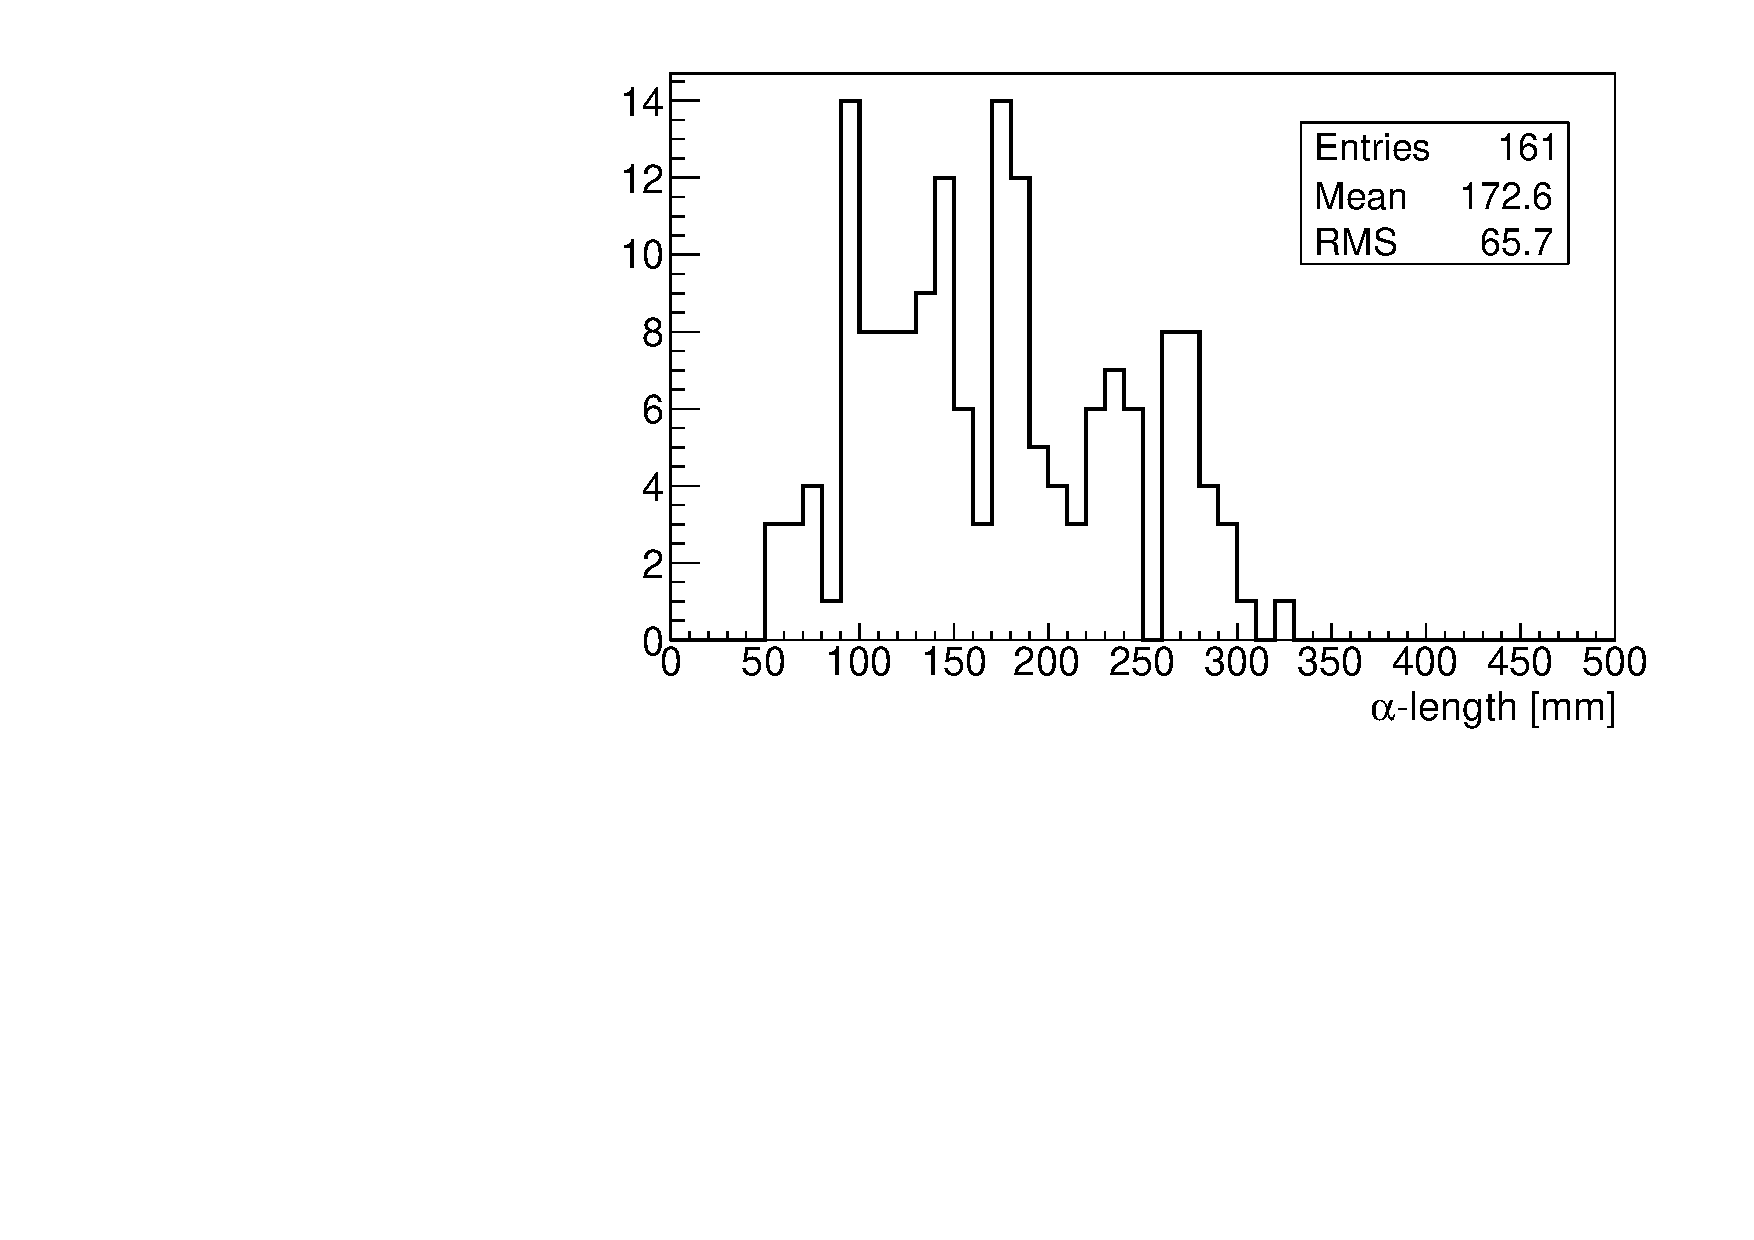
\includegraphics[scale=0.38]{pictures/Chap5/length_alpha_tracker_selection_bulk.pdf}
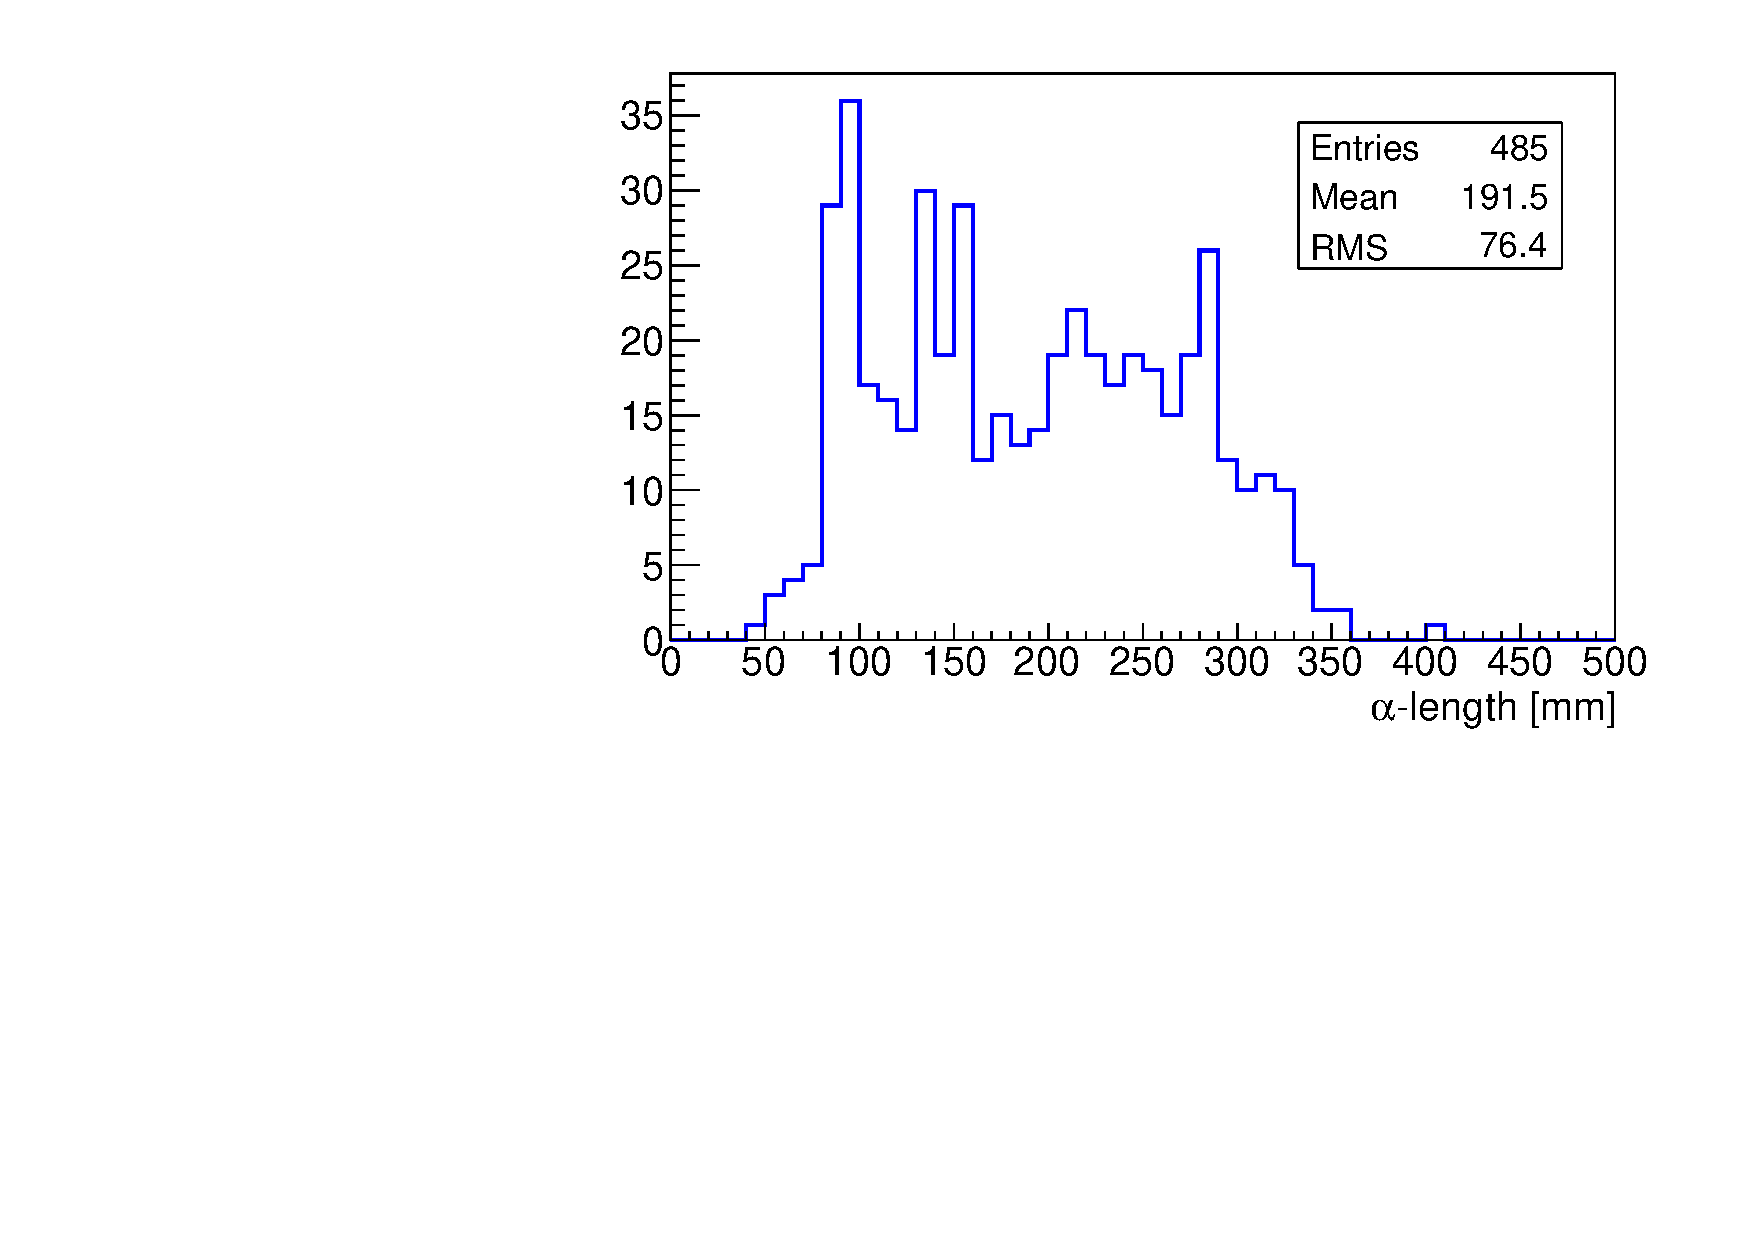
\includegraphics[scale=0.38]{pictures/Chap5/length_alpha_tracker_selection_surface.pdf}
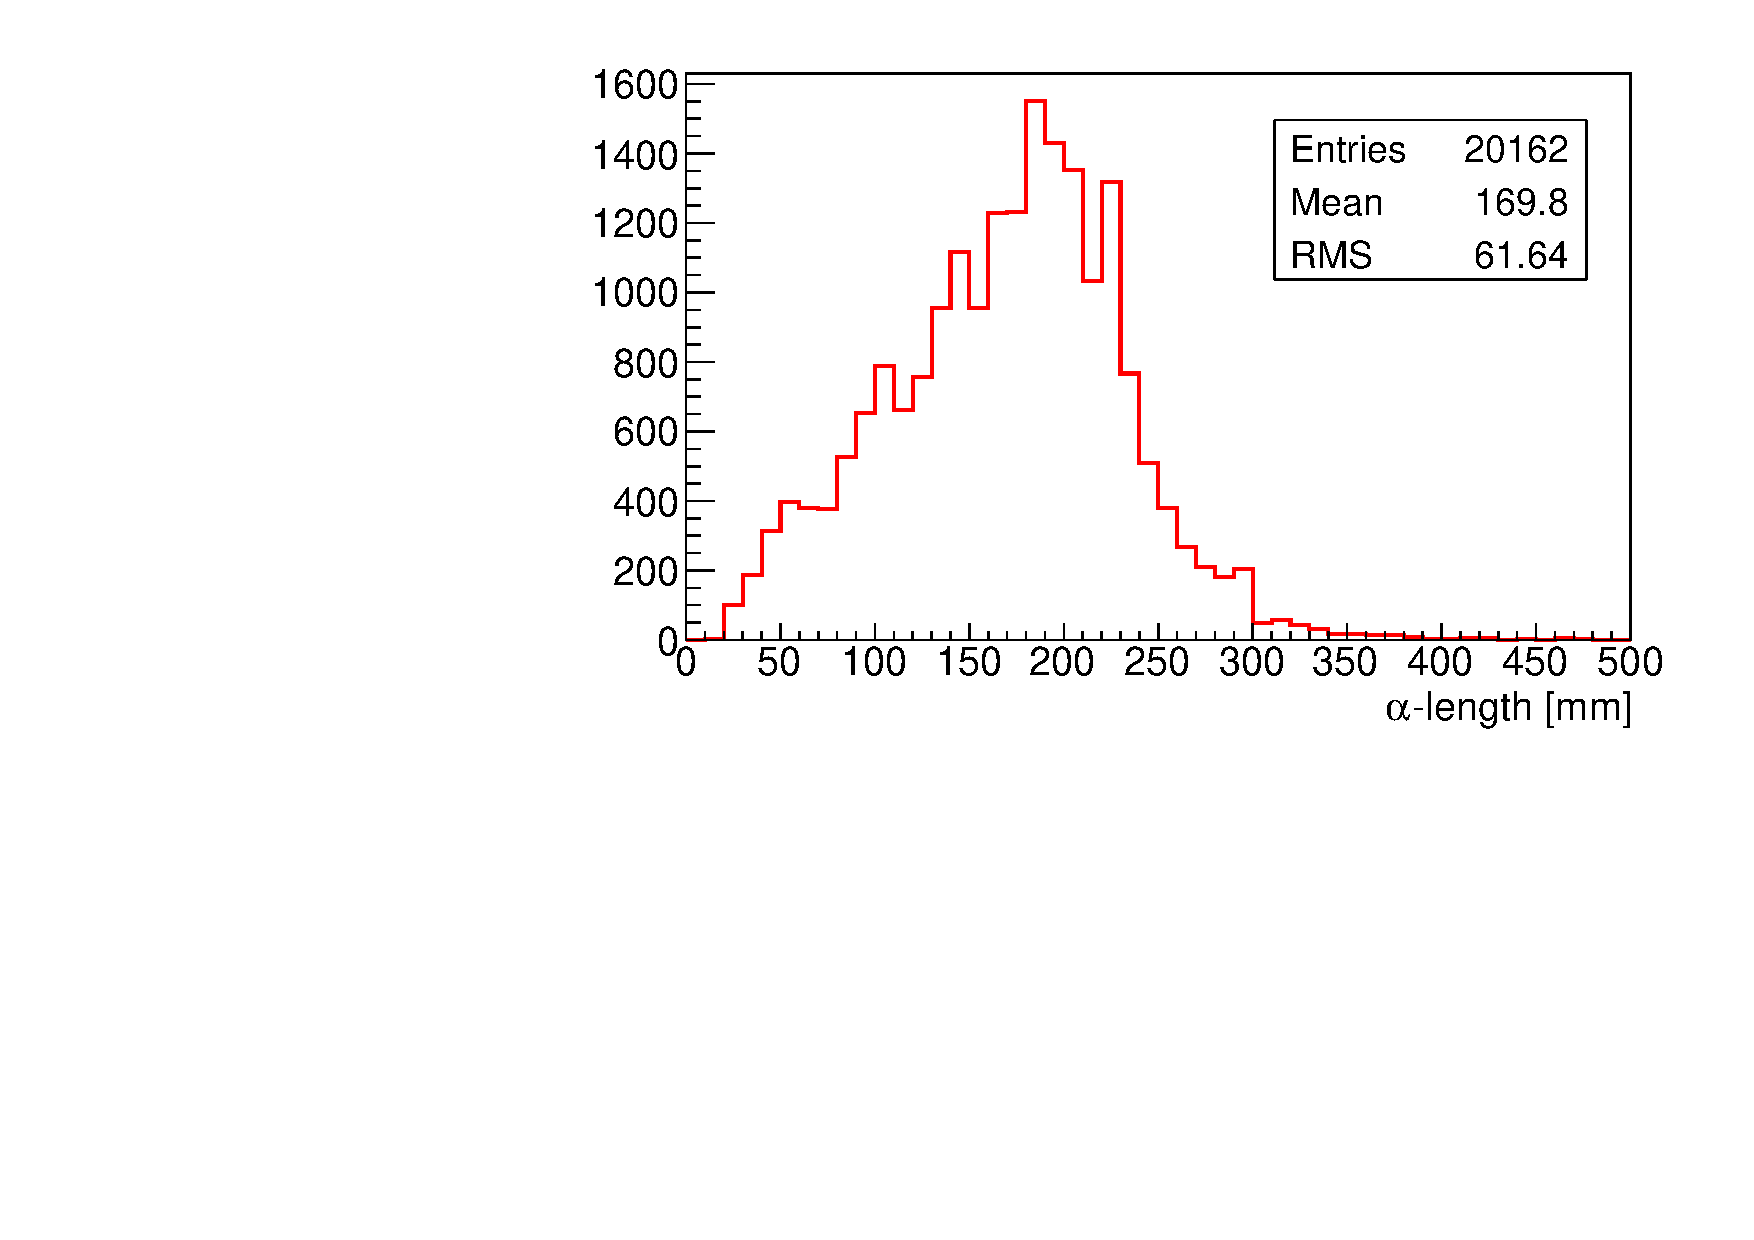
\includegraphics[scale=0.38]{pictures/Chap5/length_alpha_tracker_selection_tracker.pdf}
\caption{Alpha track length for different contributions : source bulk (black), source surface (blue) and tracker (red).}
\label{alpha_length_tracker_selection}
\end{center}
\end{figure}


\begin{figure}[h!]
\begin{center}
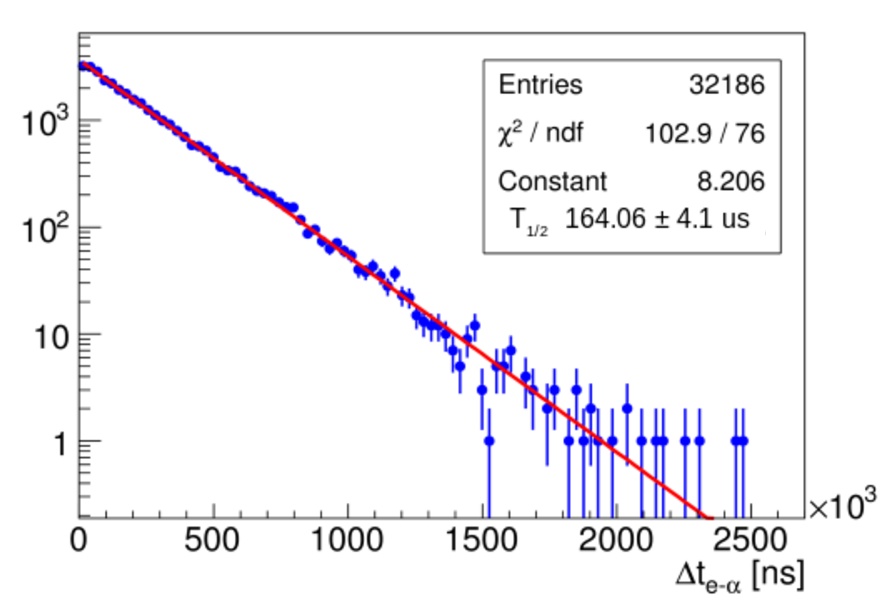
\includegraphics[scale=0.6]{pictures/Chap5/delta_t_tracker_selection_tracker.pdf}
\caption{Time between the alpha and the electron in the identified 1a1$\alpha$ channel with the tracker selection}
\label{delta_t_tracker_selection}
\end{center}
\end{figure}


\bigskip


\noindent The number of reconstructed 1e1$\alpha$ events according to the vertex is given in Table~\ref{efficiency_different_parts_tracker}. So, $\sim$7~\% of the 1e1$\alpha$ events generated in the tracker are reconstructed. The efficiency of reconstruction of the 1e1$\alpha$ events coming from the surface and the bulk is $\sim$0.2~\% and $\sim$0.05~\%. With the tracker selection, the efficiency of reconstruction of the 1e1$\alpha$ events coming from the source is very low. These residual events are the events coming from the source foil but not hitting the first layer of wires close to the source foil. The vertex of these events are extrapolated to be in the tracker. Figure~\ref{delta_t_tracker_selection} shows the time between the alpha and the electron in the 1a1$\alpha$ channel with the tracker selection. The half-life on the process is found to be 164.01 $\pm$ 4.1 $\mu$s which is in agreement with the published value~\cite{NuclearDataSheet210}. 


\begin{table}[h!]
\begin{center}
\begin{tabular}{c|c|c|c}
           & bulk   & surface & tracker \\
\hline
$\epsilon_{1e1\alpha}$ [\%] & 0.05 & 0.16  & 6.72 \\
\hline
\end{tabular}
\end{center}
\caption{Summary of the efficiency, in different parts of the detector, computed with the Monte-Carlo.}
\label{efficiency_different_parts_tracker}
\end{table}


%----------------------------------------------------------------------------------------
%    MEASUREMENTS
%----------------------------------------------------------------------------------------

\section{Measurement}\label{sec:MeasurementStategy}

\noindent In order to distinguish the contributions coming from the source foil (bulk and surface) and the tracker, the length of the alpha track is used. The strategy used to compute, for each contribution, the number of expected events and their relative error is described here. As an example, the method is explained using the source selection.


\bigskip


\noindent \textbf{1) Normalization to the activity and sum} : The three distributions of the alpha track length given in Figure~\ref{alpha_length_source_selection} are normalized to their respective activities computed in Section~\ref{sec:ActivityComputation} and summed. Figure~\ref{ref_distribution} shows the summed distribution.


\begin{figure}[h!]
\begin{center}
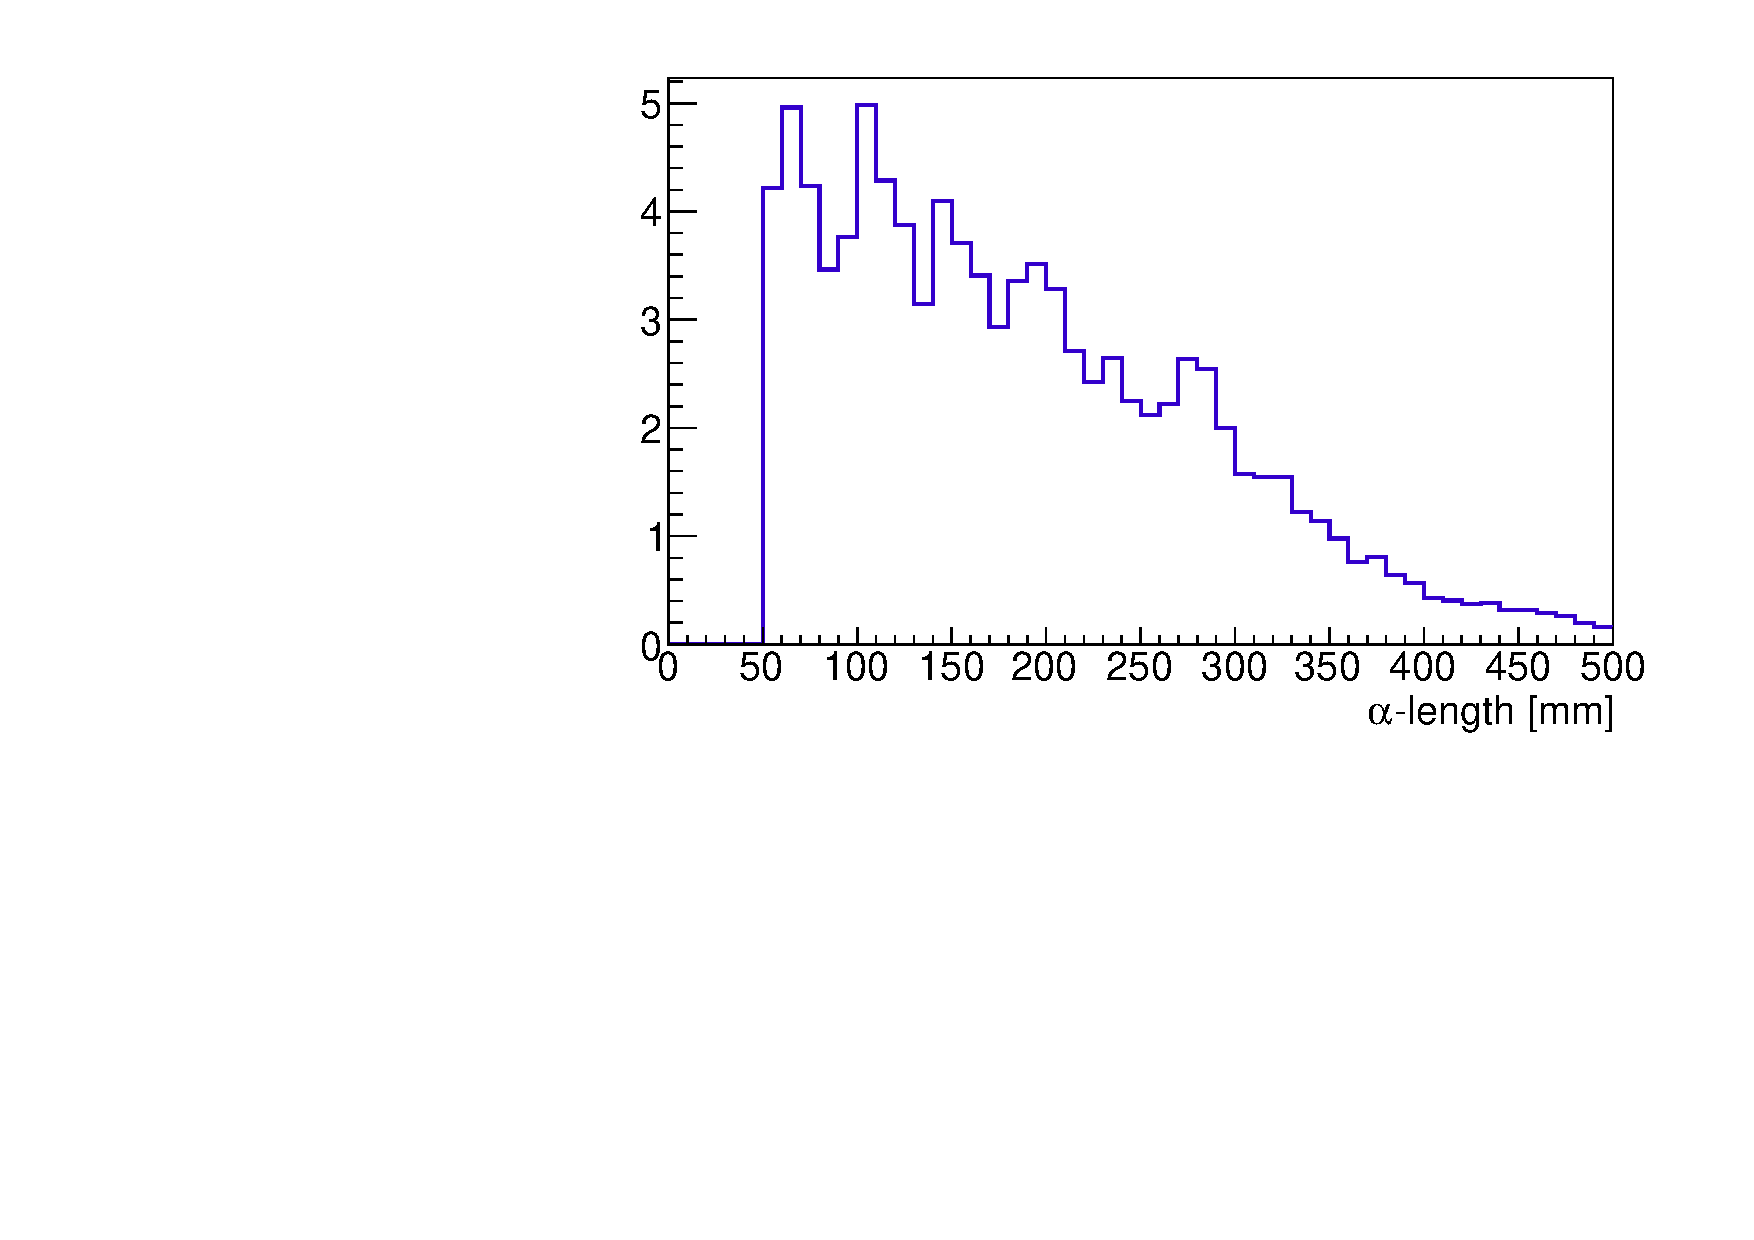
\includegraphics[scale=0.55]{pictures/Chap5/basic_distribution_alpha_length.pdf}
\caption{Summed and normalized alpha length distribution from the 3 contributions (source bulk, source surface and tracker).}
\label{ref_distribution}
\end{center}
\end{figure}


\bigskip


\noindent \textbf{2) Normalization to the exposure} : The previous distribution is normalized to a given exposure. The final distribution is obtained.


\bigskip


\noindent \textbf{3) Generation of a pseudo experiment} : From this final distribution a pseudo experiment is generated. To mimic the real data, the number of expected events is a random number according to Poissonian law. Figure~\ref{pseudo-experiment} shows a pseudo experiment after an exposure of 60 days.


\begin{figure}[h!]
\begin{center}
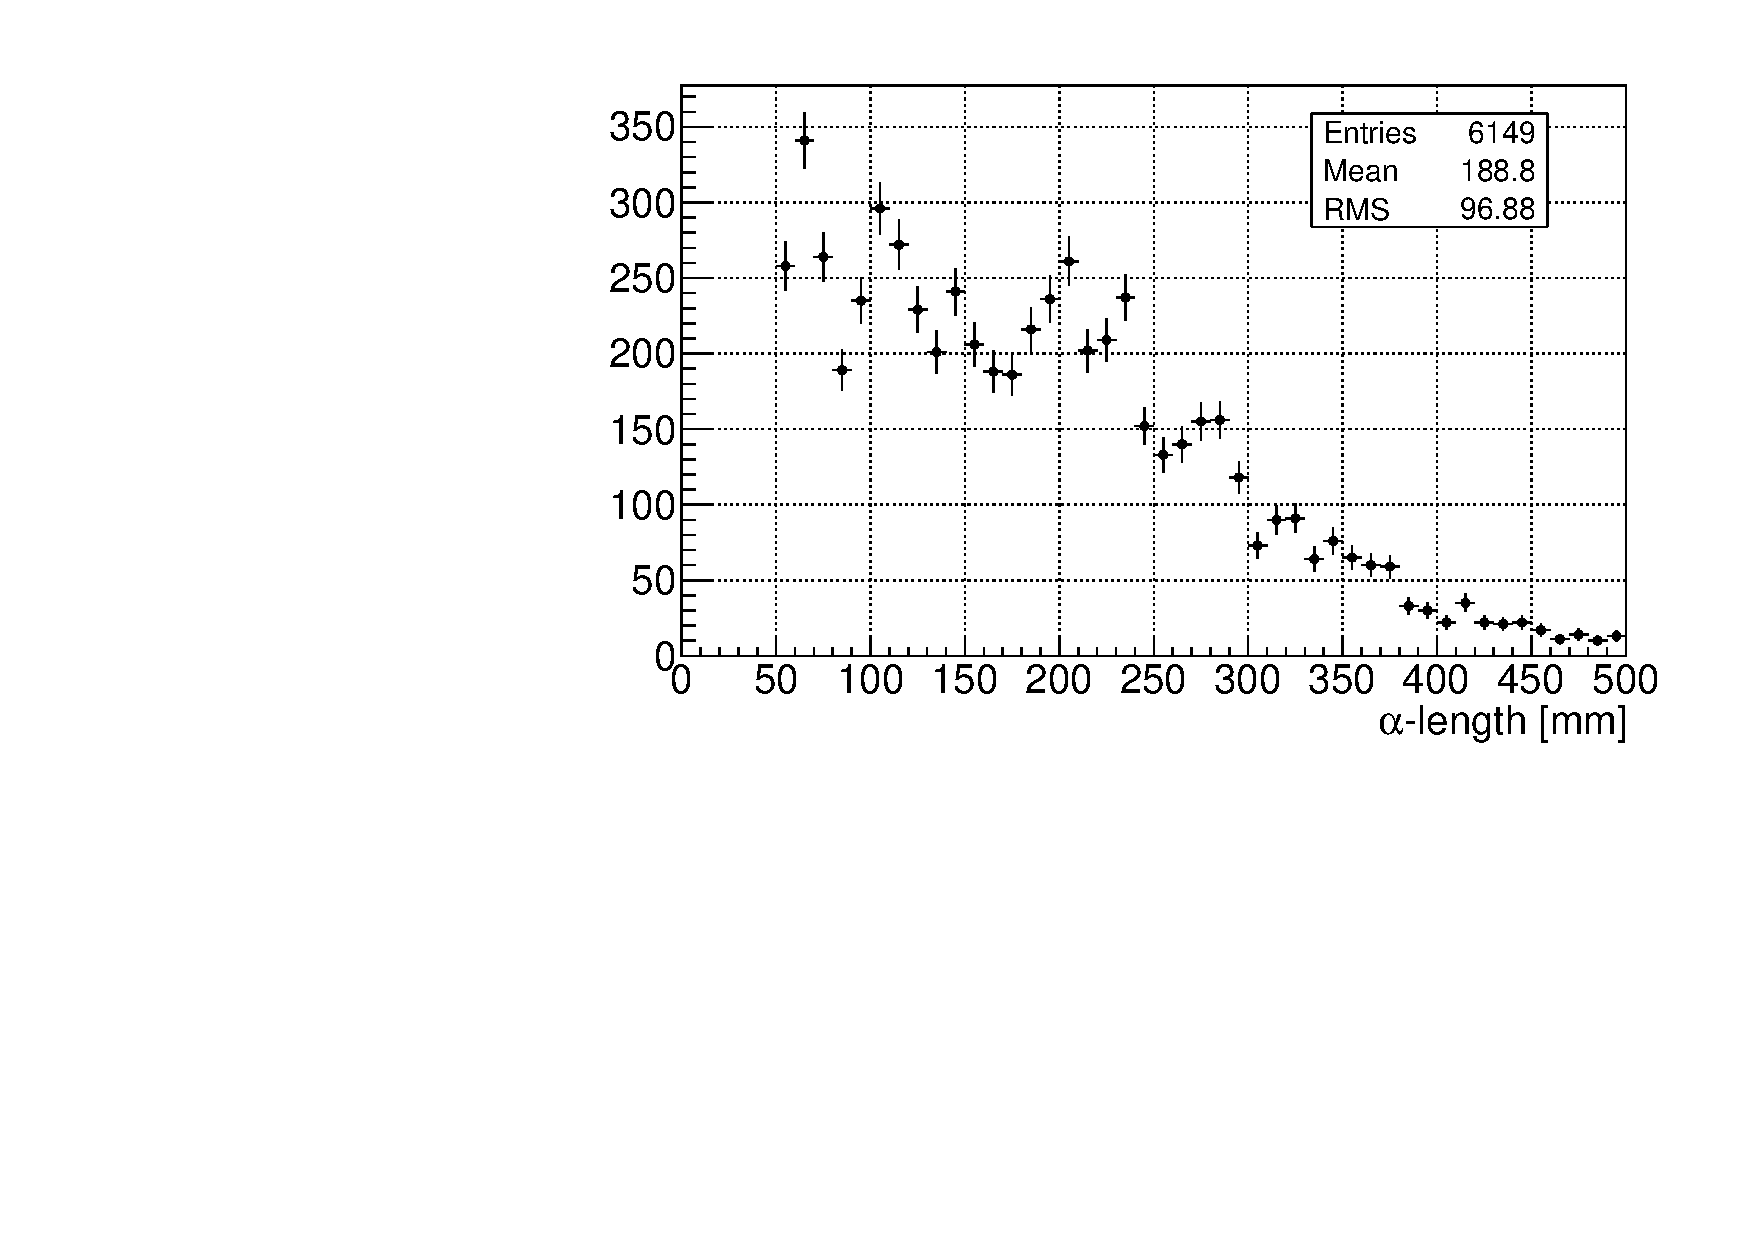
\includegraphics[scale=0.50]{pictures/Chap5/alph_length_exposure_60.pdf}
\caption{Pseudo experiment, length of the $\alpha$ track after an exposure of 60 days.}
\label{pseudo-experiment}
\end{center}
\end{figure}


\bigskip


\noindent \textbf{4) Fit the pseudo-experiment} : The pseudo-experiment is fitted with the three distributions presented in Section~\ref{sec:Selection1e1aChannel}. The fit is a likelihood fit (\`a la NEMO 3) which returns the activity of each component. Figure~\ref{fit-pseudo-experiment} shows the result of the fit.


\begin{figure}[h!]
\begin{center}
\includegraphics[scale=0.5]{pictures/Chap5/fit_exposure_60_v1.pdf}
\caption{Fit of the pseudo-experiment with the three contributions after an exposure of 60~days. In red, the tracker contribution. In blue, the surface contribution. In black, the bulk contribution.}
\label{fit-pseudo-experiment}
\end{center}
\end{figure}


\bigskip


\noindent \textbf{5) Repeat 3 and 4} : The actions 3 and 4 are repeated 10$^\text{5}$ times. The distribution of the fitted activity of each component is plotted in~Figure~\ref{gaus}. The mean activity ($\mu$) and the sigma ($\sigma$) are recoverered. The relative error is defined as the ratio~:~$\sigma$~/~$\mu$.

\begin{figure}[h!]
\begin{center}
\includegraphics[scale=0.45]{pictures/Chap5/gaussian_bulk_activity_v1.pdf}
\caption{Distribution of the fitted activities for the bulk contribution}
\label{gaus}
\end{center}
\end{figure}


\FloatBarrier
%For each contribution, knowing the measured activities computed in Section~2 and the efficiency of reconstruction presented in Section~5, the number of expected events is computed according eq~\ref{eq_number_of_expected_events}.



%----------------------------------------------------------------------------------------
%    RESULTS AND CONCLUSION
%----------------------------------------------------------------------------------------

\section{Results and Conclusion}\label{sec:Results}


\noindent The method described in Section~\ref{sec:MeasurementStategy} is generalized to different exposures. For both selections, source and tracker, the number of expected events is computed according to Eq.\ref{eq_number_of_expected_events} and by using the selection efficiency presented in Section~\ref{sec:Selection1e1aChannel} and the mean activity computed in Section~\ref{sec:MeasurementStategy}.


\subsection{Source selection}


\NI Concerning the source selection, the number of events according to the exposure for the different contributions is shown in Figure~\ref{picture_number_of_expected_events_source_selection}. Table~\ref{table_number_of_expected_events_source_selection} summarizes the number of expected events after 1~day, 1~week, 2~weeks and 1~month with the source selection. The relative error defined as the ratio $\sigma$/$\mu$ is computed for different exposures and shown in Figure~\ref{picture_relative_error_source_selection}. Table~\ref{table_relative_error_source_selection} gives the results at some exposures.


\begin{table}[h!]
\begin{center}
\begin{tabular}{l|c|c|c|c}
 & $\symbol{64}$ 1 day  & $\symbol{64}$ 1 week  & $\symbol{64}$ 2 weeks & $\symbol{64}$ 1 month  \\
\hline
$\text{N}_\text{bulk}$ [cts.]    & $\sim$ 40 & $\sim$ 275  & $\sim$ 600 & $\sim$ 1175 \\
$\text{N}_\text{surface}$ [cts.] & $\sim$ 2  & $\sim$ 10   & $\sim$ 25  & $\sim$ 50   \\
$\text{N}_\text{tracker}$ [cts.] & $\sim$ 60 & $\sim$ 420  & $\sim$ 900 & $\sim$ 1800 \\
\hline
\end{tabular}
\end{center}
\caption{Number of expected events vs the exposure time for the different contributions using the source selection.}
\label{table_number_of_expected_events_source_selection}
\end{table}


\begin{table}[h!]
\begin{center}
\begin{tabular}{l|c|c|c|c}
      & $\symbol{64}$ 1 day  & $\symbol{64}$ 1 week  & $\symbol{64}$ 2 weeks & $\symbol{64}$ 1 month  \\
\hline
$(\sigma / \mu)_{\text{bulk}}$    & 24.9 \% & 9.4  \% & 6.4  \% & 4.5  \% \\
%$(\sigma / \mu)_{\text{surface}}$ & 84.8 $\%$ & 29.4 $\%$ & 19.9 $\%$ & 14.1 $\%$ \\
$(\sigma / \mu)_{\text{surface}}$ & 279  \% & 129  \% & 88.6 \% & 63.0 \% \\
$(\sigma / \mu)_{\text{tracker}}$ & 18.0 \% & 6.8  \% & 4.7  \% & 3.3  \% \\
\hline
\end{tabular}
\end{center}
\caption{Relative errors vs the exposure time for the different contributions using the source selection.}
\label{table_relative_error_source_selection}
\end{table}



\begin{figure}[h!]
\begin{center}
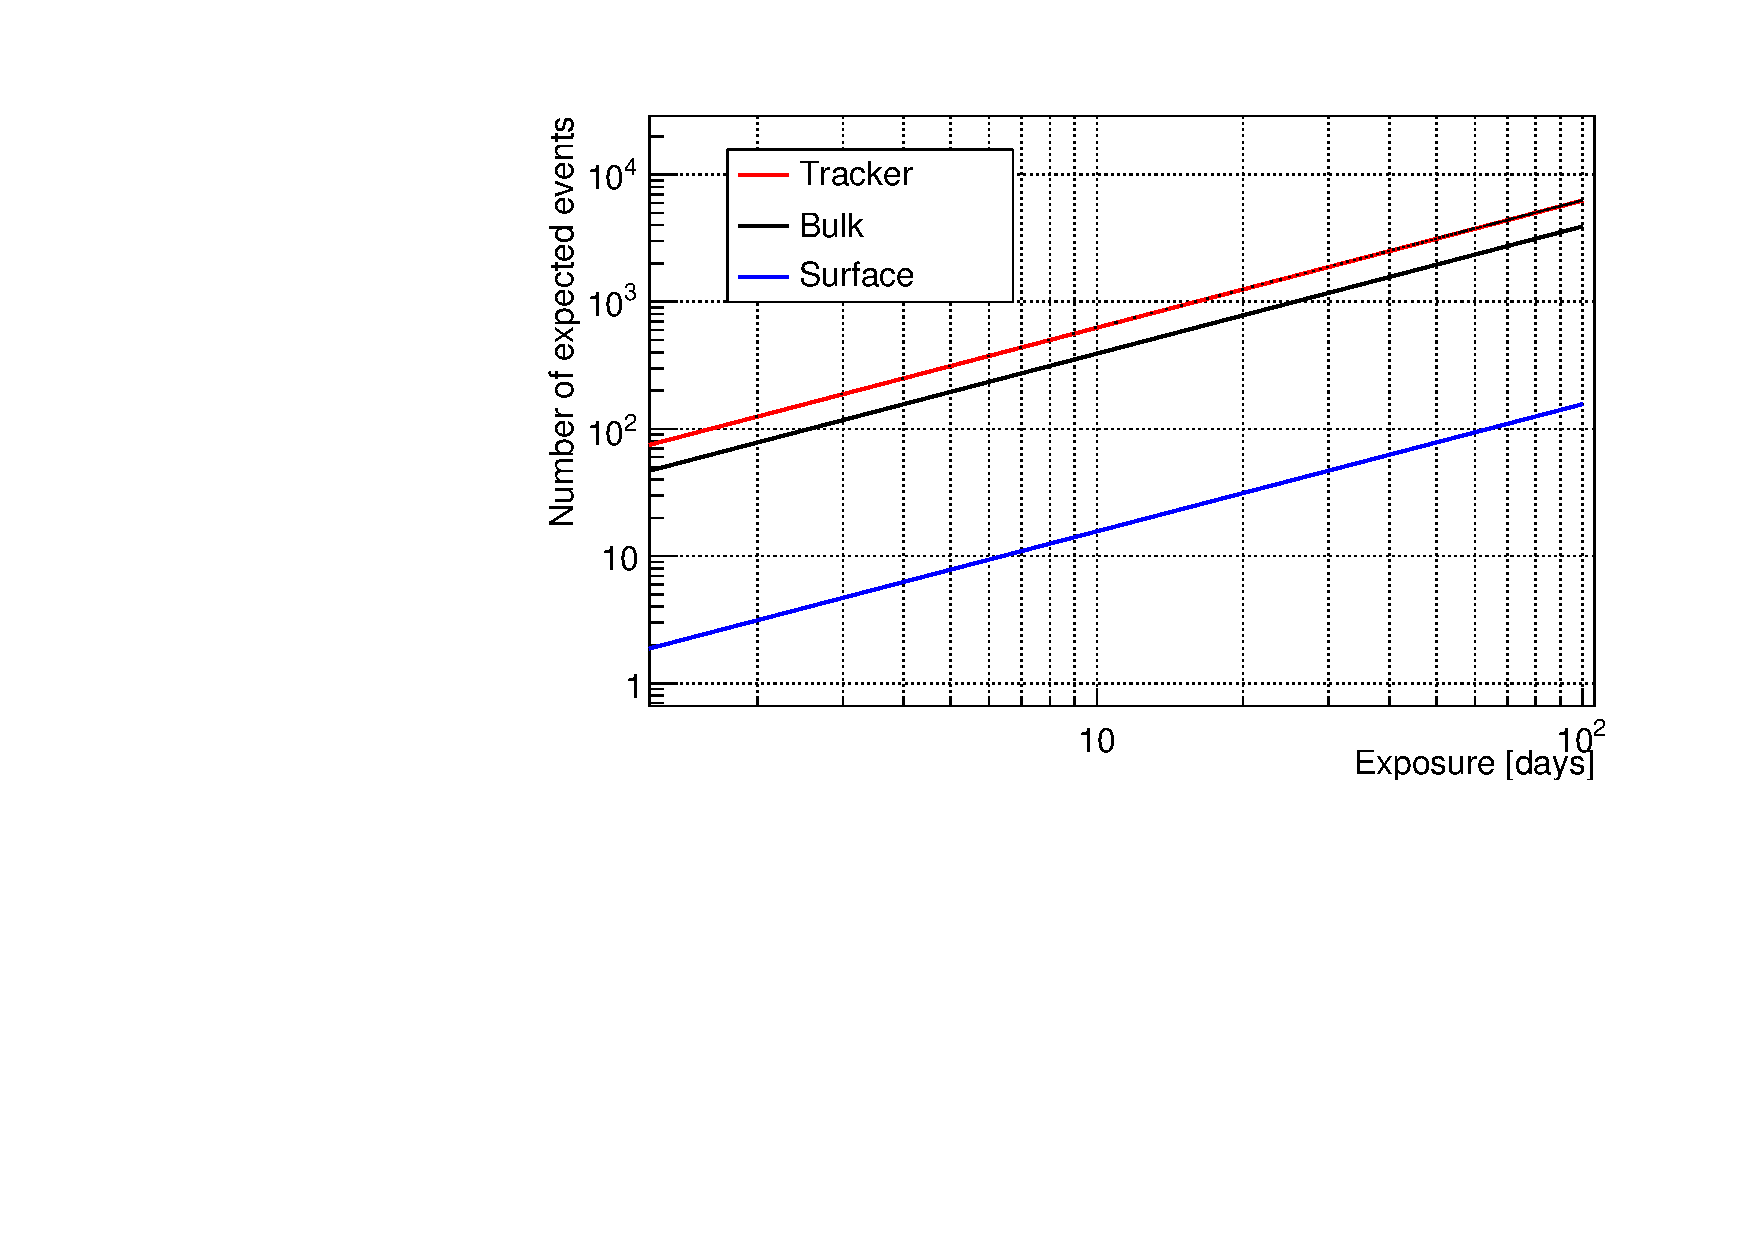
\includegraphics[scale=0.6]{pictures/Chap5/nexpected_source_selection.pdf}
\caption{Number of expected events vs the exposure time for the different contributions using the source selection.}
\label{picture_number_of_expected_events_source_selection}
\end{center}
\end{figure}


\begin{figure}[h!]
\begin{center}
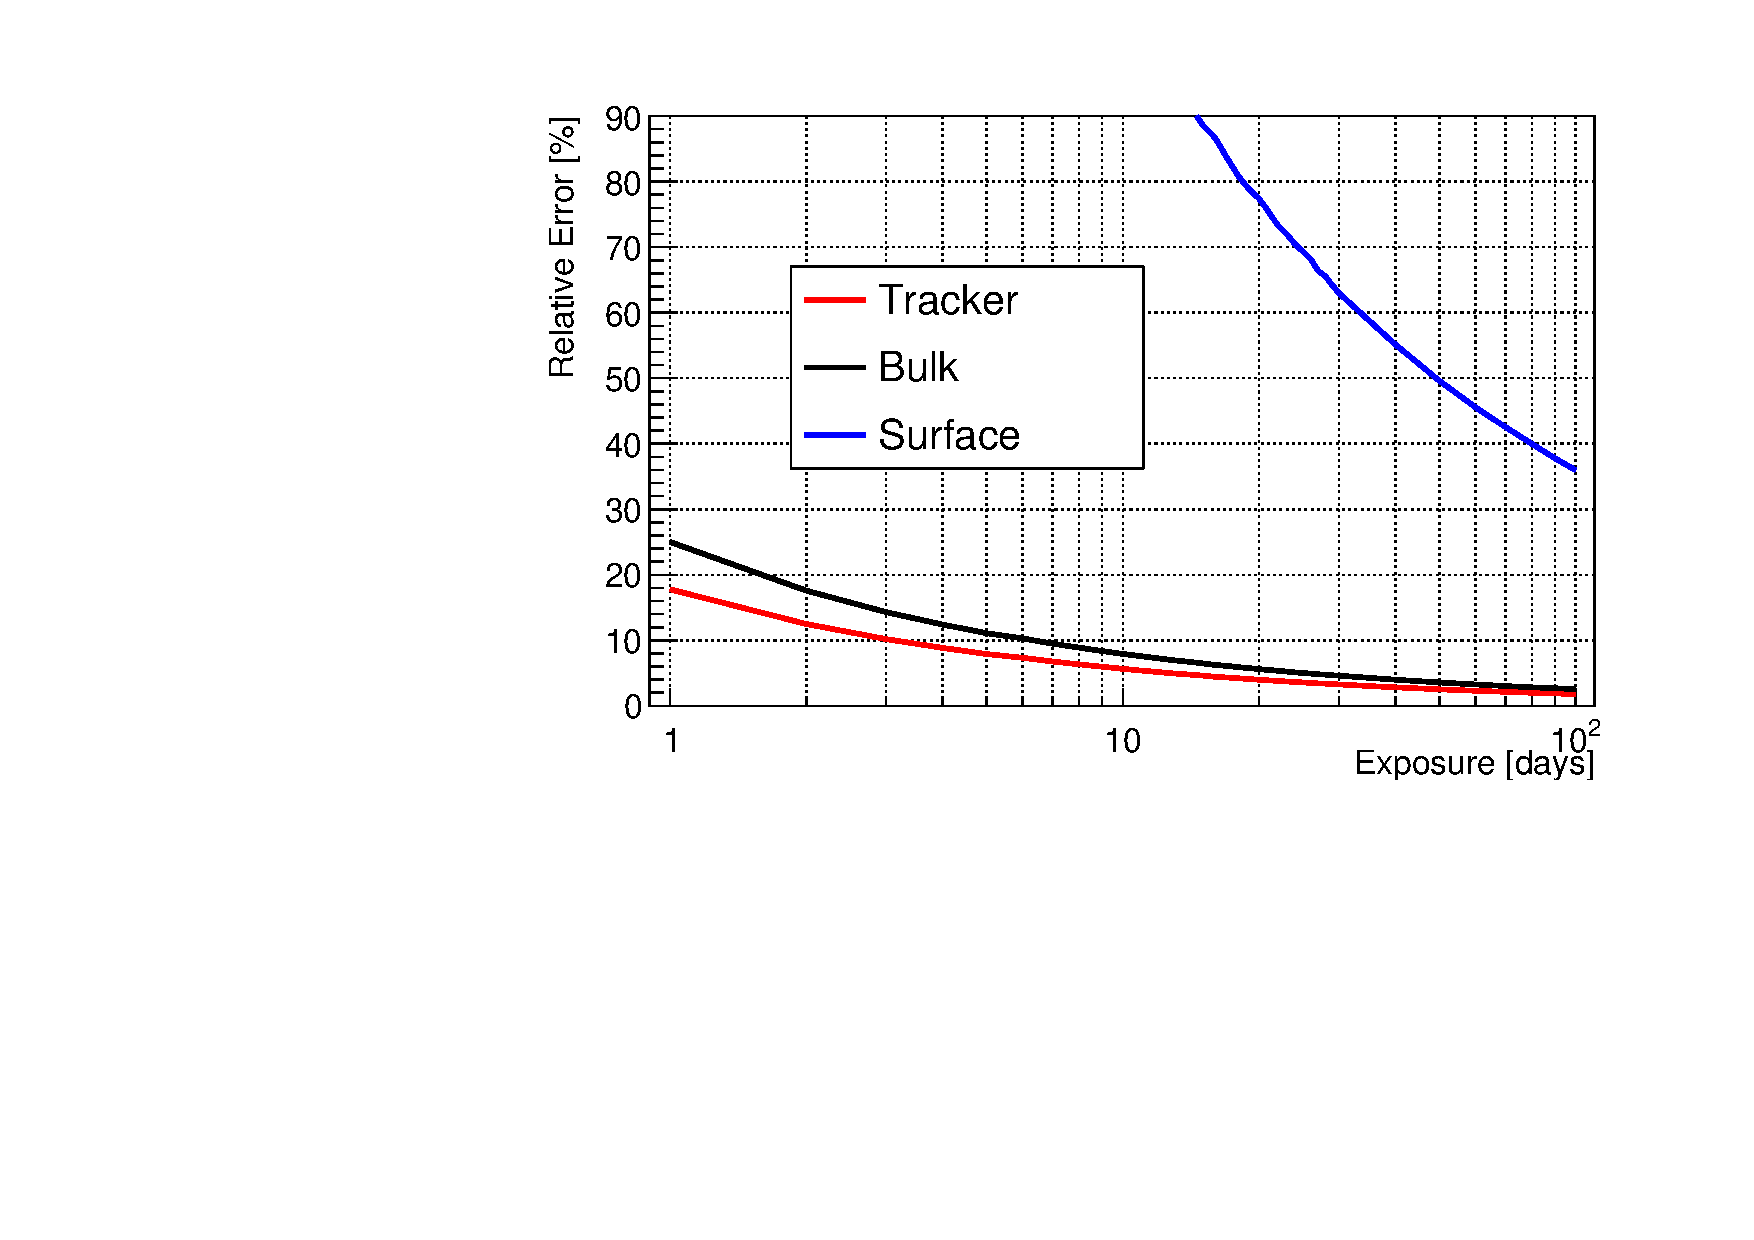
\includegraphics[scale=0.6]{pictures/Chap5/n_source_selection_last_results.pdf}
\caption{Relative errors using the source selection vs the exposure.}
\label{picture_relative_error_source_selection}
\end{center}
\end{figure}




\bigskip

\noindent With the source selection, the level of $^{\text{214}}$Bi background coming from the source bulk can be known at $\sim$ 10~\% after one week of data taking. The level of $^{\text{214}}$Bi background coming from the surface of the foil, due to its very low activity compared to the other contributions, is expected to be measured with a high uncertainty, $\sim$~63\% after one month of data taking. Note that this value is a bit pessemistic since this study does not take into account that a fraction of the $^{\text{222}}$Rn inside the tracker can be transferred to the foil surface. Futhermore, new radon emanation  measurements of the tracker show that the activity of the tracker has been a little bit overestimated in this work. Finally, note that even if the source selection is not optimised to measure the background contribution from the tracker, it can be measured at $\sim$ 7~\% after one week of data taking.  


\FloatBarrier


\subsection{Tracker selection}


\noindent For the tracker selection, the number of expected events according to the exposure is plotted in Figure~\ref{picture_number_of_expected_events_tracker_selection} and the relative errors are shown in Figure~\ref{picture_relative_error_tracker_selection}. Table~\ref{table_number_of_expected_events_relative_error_tracker_selection} summaries the results for several different exposures. The level of $^{\text{222}}$Rn inside the tracker can be known at $\sim$ 8\% after one day and can be monitored daily. Moreover, as this selection is not optimised for the events coming from the bulk and the surface of the foil, the selection efficiencies are low and the expected number of events coming from the foil are negligible. The measurement of the level of $^{\text{222}}$Rn in the tracker volume will be one of the measurements to be performed.


 


\begin{figure}[h!]
\begin{center}
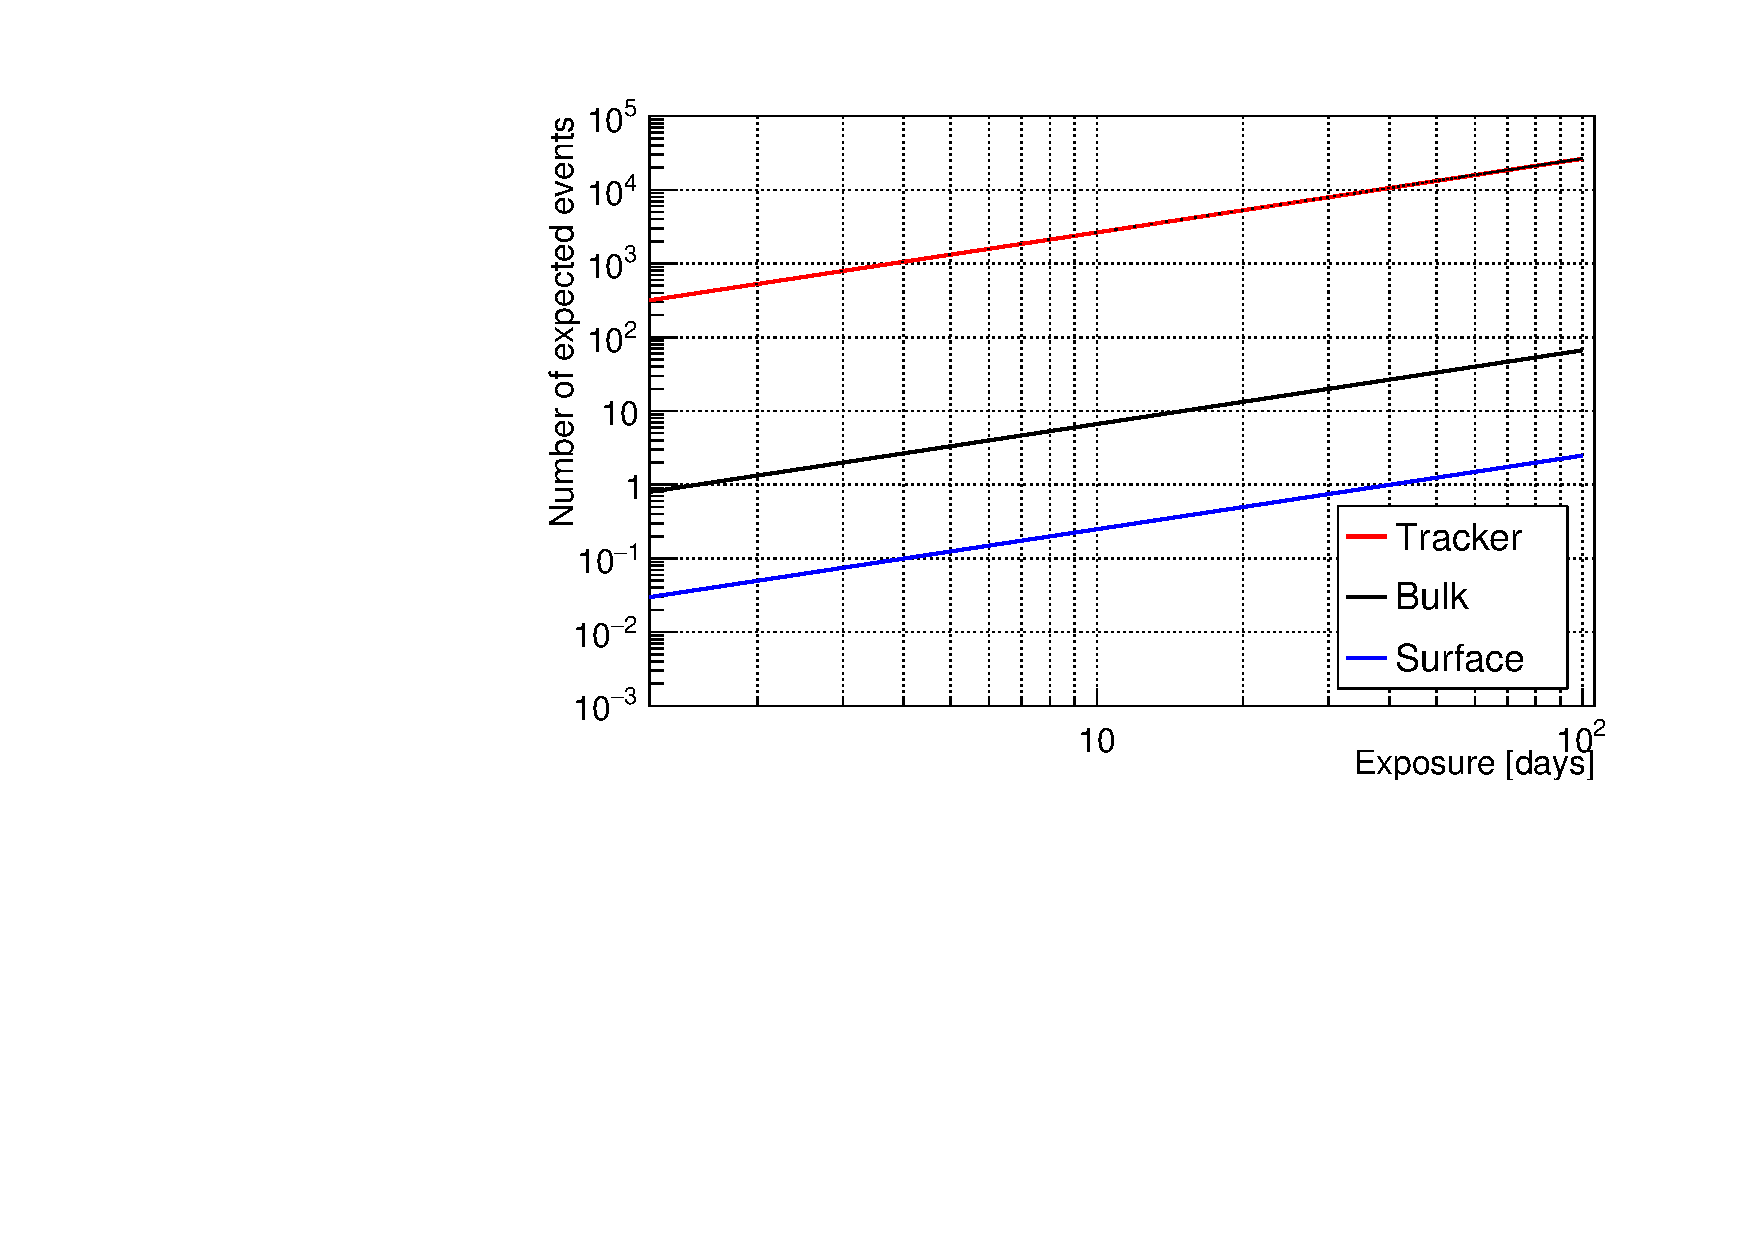
\includegraphics[scale=0.5]{pictures/Chap5/nexpected_tracker_selection.pdf}
\caption{Number of expected events vs the exposure time for the different contributions using the tracker selection.}
\label{picture_number_of_expected_events_tracker_selection}
\end{center}
\end{figure}

\begin{figure}[h!]
\begin{center}
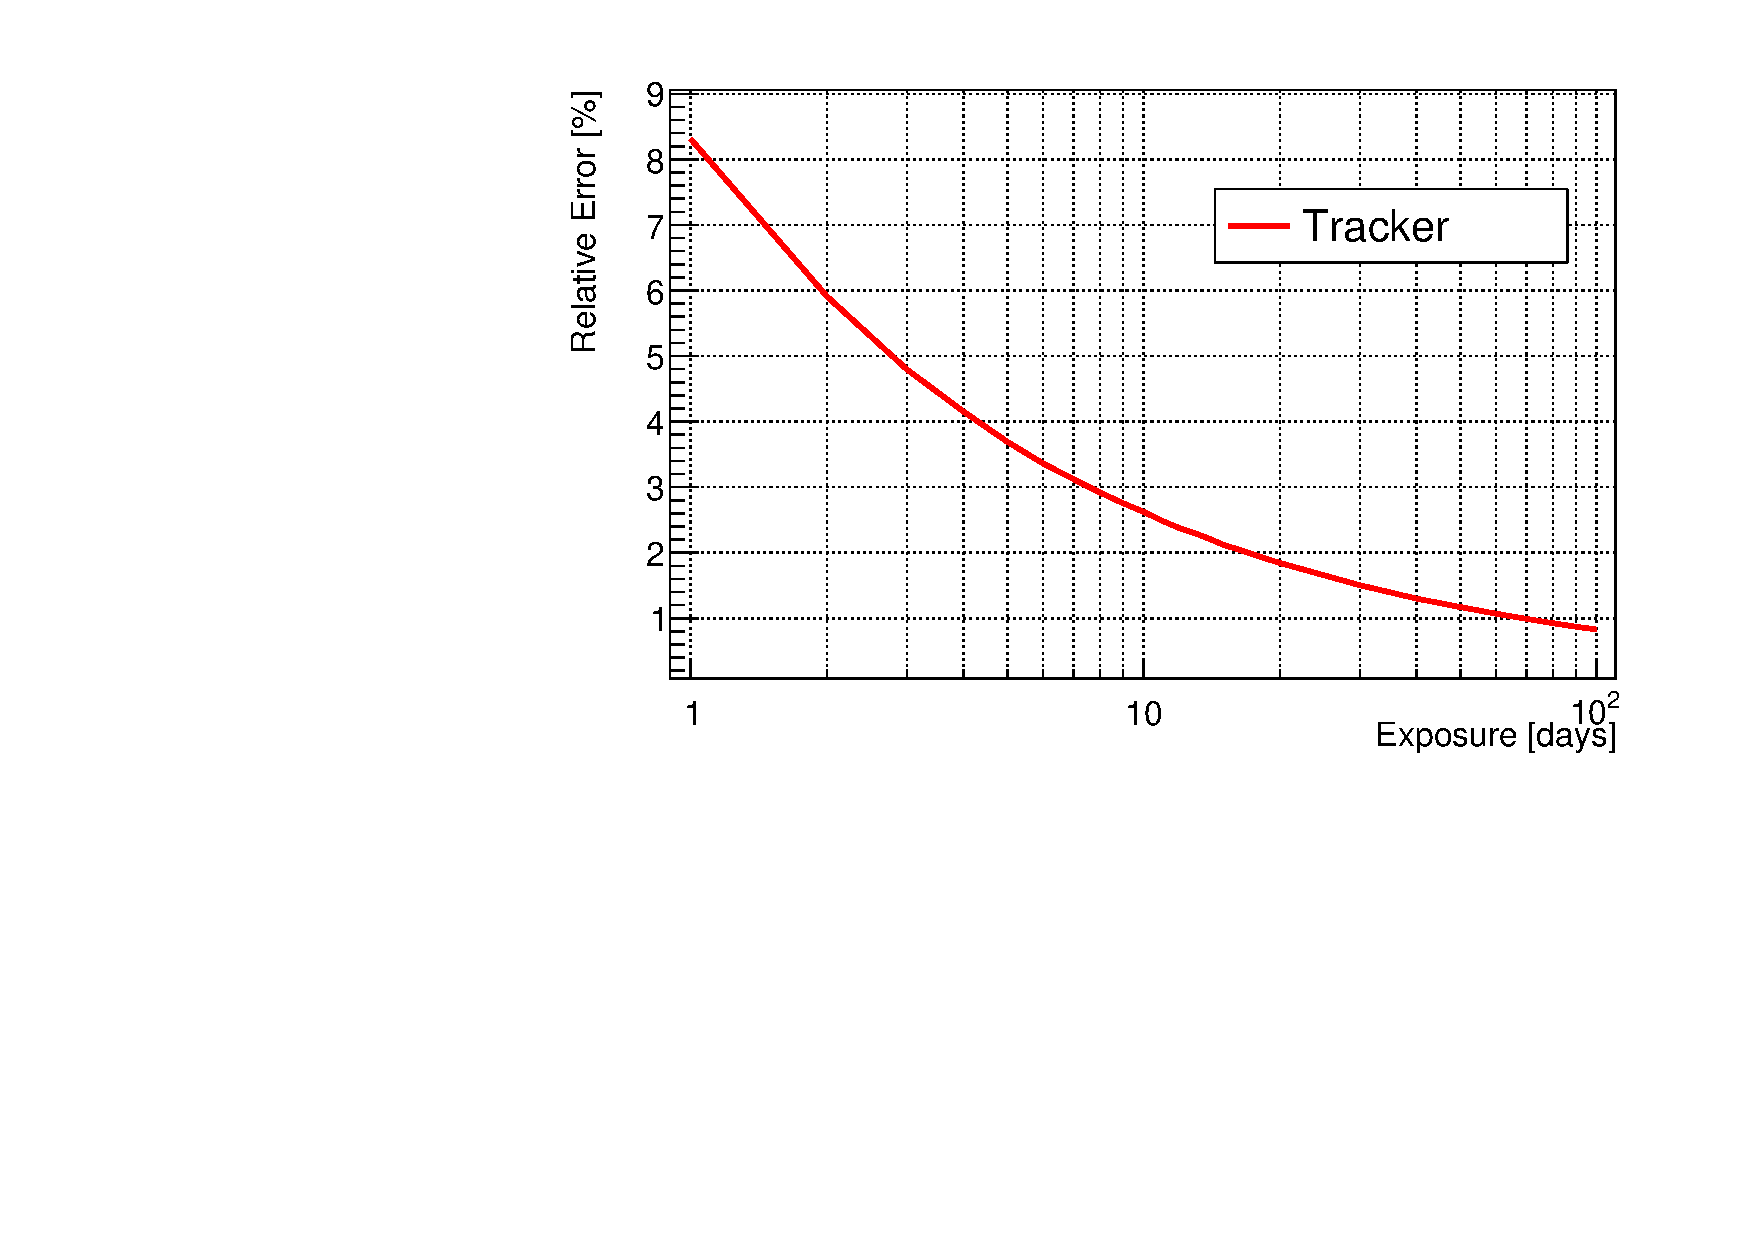
\includegraphics[scale=0.5]{pictures/Chap5/rr.pdf}
\caption{Relative errors using the tracker selection vs the exposure.}
\label{picture_relative_error_tracker_selection}
\end{center}
\end{figure}


\begin{table}[h!]
\begin{center}
\begin{tabular}{l|c|c|c|c}
      & $\symbol{64}~$1 day  & $\symbol{64}~$1 week  & $\symbol{64}~$2 weeks & $\symbol{64}~$1 month  \\
\hline
$\text{N}_\text{tracker}$         & $\sim$ 265 & $\sim$ 1860 & $\sim$ 4000 & $\sim$ 8000 \\ 
$(\sigma / \mu)_{\text{tracker}}$ & 8.3 \%     & 3.1  \%     & 2.1  \%     & 1.5  \% \\
\hline
\end{tabular}
\end{center}
\caption{Number of expected events and relative errors in tracker vs the exposure time for the tracker selection.}
\label{table_number_of_expected_events_relative_error_tracker_selection}
\end{table}


\bigskip
\FloatBarrier


%\noindent The study of the 1e1$\alpha$ channel has been presented in this note. The computation of the expected activity has been presented in~Section~2. The software tools used for the simulation and the reconstruction have been presented in Section~3. Section~4 presents the reconstruction of the $\alpha$ particles. The alpha finder algorithm is also presented. Section~5 presents the selection of the 1e1$\alpha$ events. The measurement and the strategy to measure a certain amount of $^{222}$Rn are described in Section~6.


\bigskip


\noindent According to the efficiency of reconstruction of the 1e1$\alpha$ channel and the different activities measured by the collaboration, the number of expected events due to the $^{\text{222}}$Rn can be computed. The level of $^{\text{222}}$Rn coming from the tracker can be known at $\sim$8~\% after one day of measurement, so, it can be measured daily. The level of $^{\text{222}}$Rn coming from the foil bulk can be known at $\sim$10~\% after one week of measurement.


\end{document}
